\chapter[$\Htautaulh$ strategy][$\Htautaulh$ strategy]{$\Htautaulh$ strategy}
\label{chap:strategy}

\begin{quote}
  The strategy of the $\Htautaulh$ analysis is described. This draws from documentation detailing its evolution in recent years~\cite{ATLAS-CONF-2012-160,ATLAS-CONF-2013-108}, especially the recent ATLAS $\Htautau$ publication~\cite{HIGG-2013-32}.
\end{quote}

\section{Introduction}
\label{sec:strategy-introduction}

The search for the Higgs boson has been the major focus of accelerator physics for decades. Though explored in great detail at experiments at LEP~\cite{2003.lep-higgs} and the Tevatron~\cite{2013.tevatron-higgs}, its existence has only recently proven by the ATLAS and CMS experiments at the LHC.

\subsection{ATLAS Higgs program}
\label{sec:strategy-higgs}

The ATLAS Higgs program initially focused on five decay modes expected to have sensitivity to Standard Model Higgs production in the first years of LHC data-taking: $\Hyy$, $\HZZ$, $\HWW$, $\Htautau$, and $\Hbb$. The $\Hyy$ and $\HZZ$ analyses are appealing for their distinctive signatures, and the $\HWW$, $\Htautau$, and $\Hbb$ analyses are appealing for their relatively high rates. The predicted Higgs branching fractions for selected decay modes are given in \cref{tab:strategy-higgs-BR}.

\begin{table}[bp]
  \centering
  \renewcommand{\arraystretch}{1.4}
  \caption{Predicted branching fractions for the Higgs boson of mass 125 GeV~\cite{higgs-branchingfractions}.}
  \begin{tabular}{c|ccc|cccc}
                     & \multicolumn{3}{c|}{fermions} & \multicolumn{4}{c}{bosons}                         \\
  \hline
  Decay mode         & $bb$ & $\tautau$ & $\mu\mu$   & $WW^\ast$ & $ZZ^\ast$ & $\gamma\gamma$ & $Z\gamma$ \\
  Branching fraction & 58\% & 6.3\%     & 0.022\%    & 22\%      & 2.6\%     & 0.23\%         & 0.15\%    \\

\end{tabular}


  \label{tab:strategy-higgs-BR}
\end{table}

\subsubsection{$\Hbosons$}

The Higgs discovery in 2012-2013 is driven by the bosonic decays. The $\Hyy$ and $\HZZ$ analyses enjoy excellent mass resolution for reconstructing $m_H$ and resonant backgrounds. They measure the Higgs mass to less than one percent uncertainty. The $\HWW$ analysis utilizes a distinctive final state (two leptons with low $\Delta\phi$) and a relatively high branching fraction. Higgs discovery plots for these analyses can be seen in \cref{fig:strategy-higgs-yyzzww}.

\begin{figure}[tp]
  \centering
  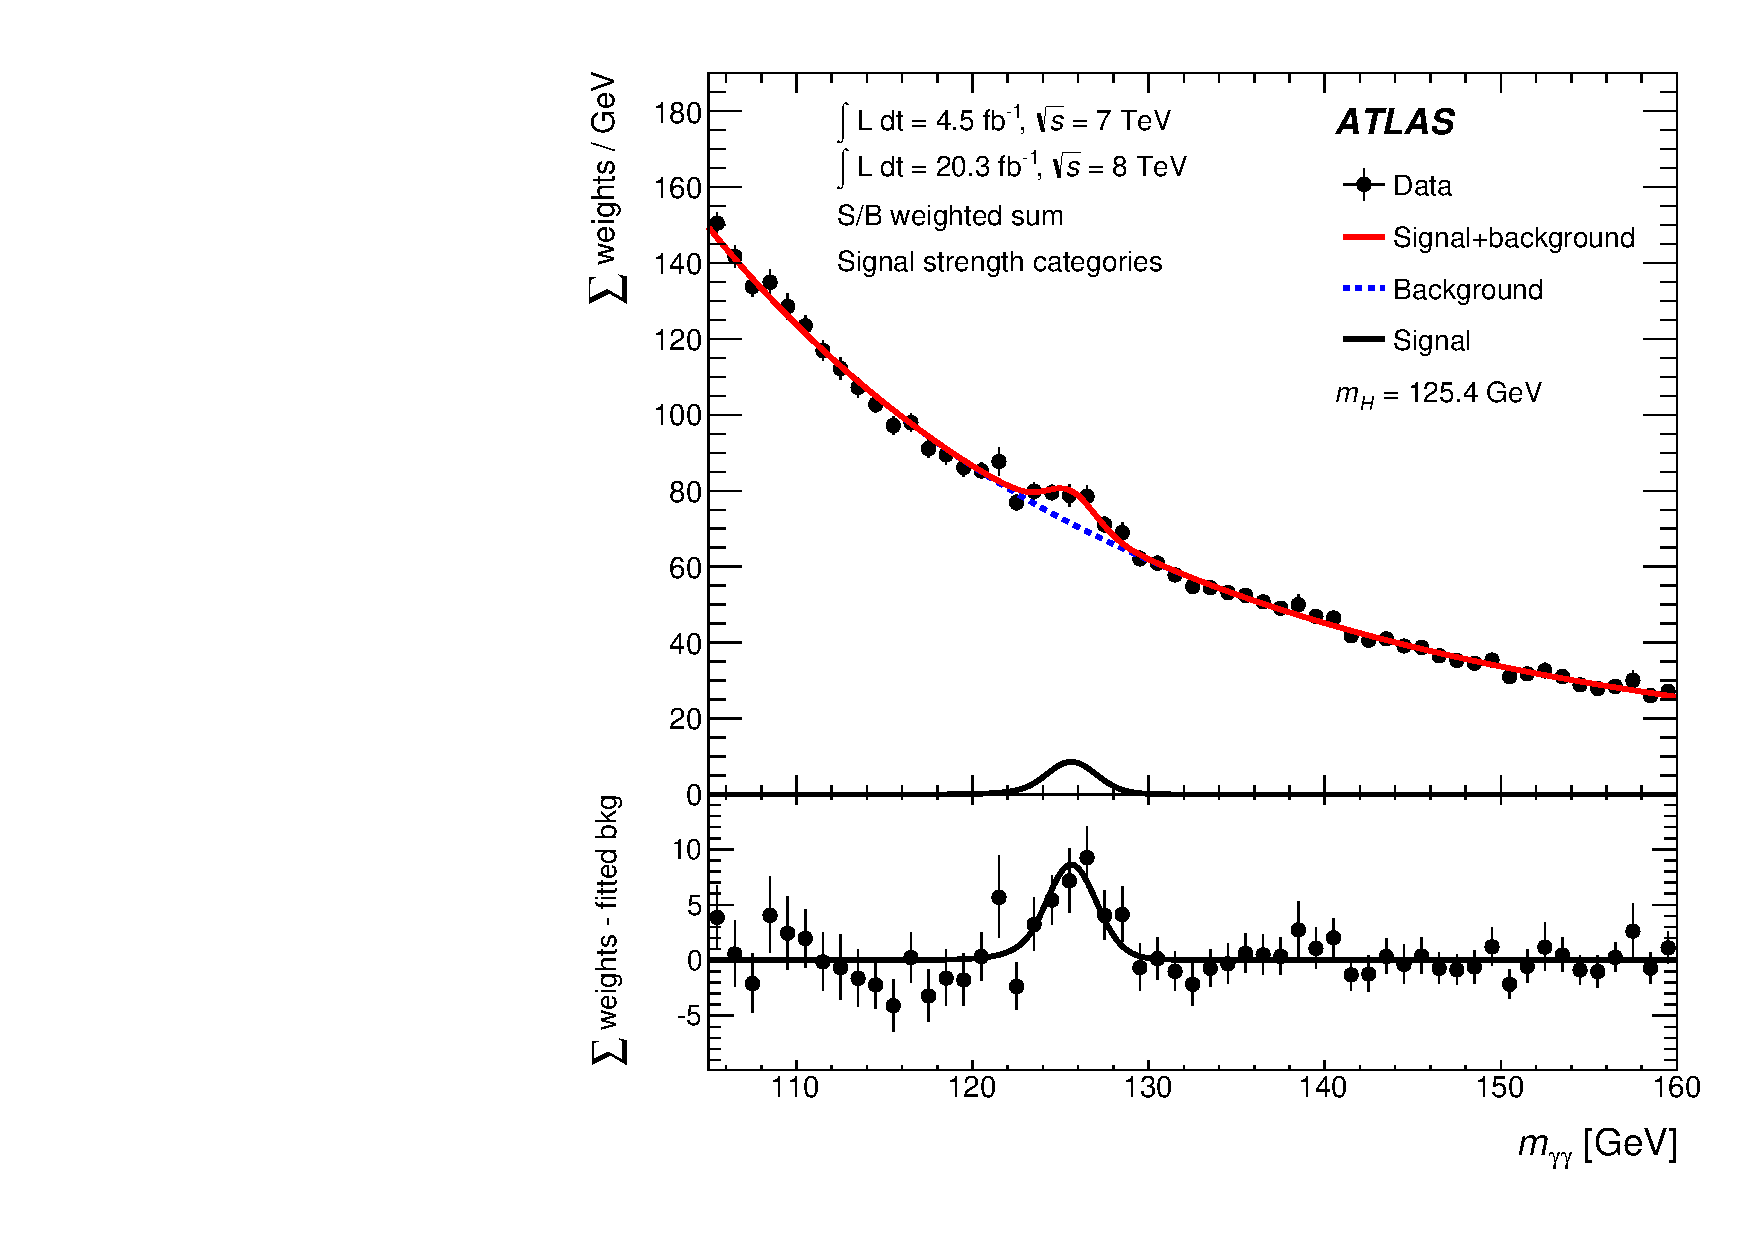
\includegraphics[width=0.32\textwidth]{figures/HIGG-2013-08/fig_13}
  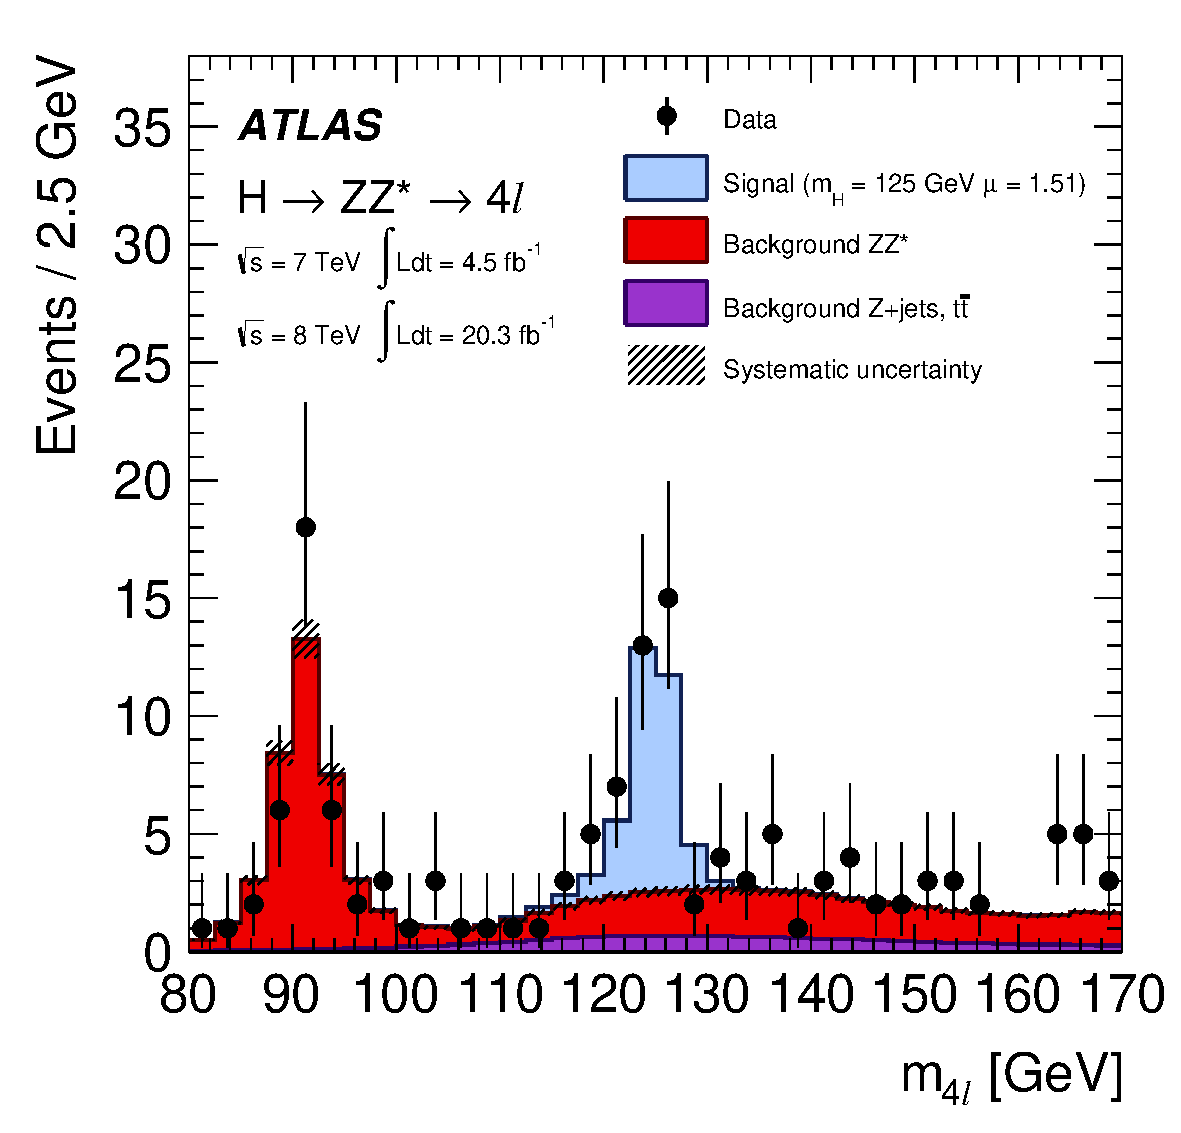
\includegraphics[width=0.32\textwidth]{figures/HIGG-2013-21/fig_13a}
  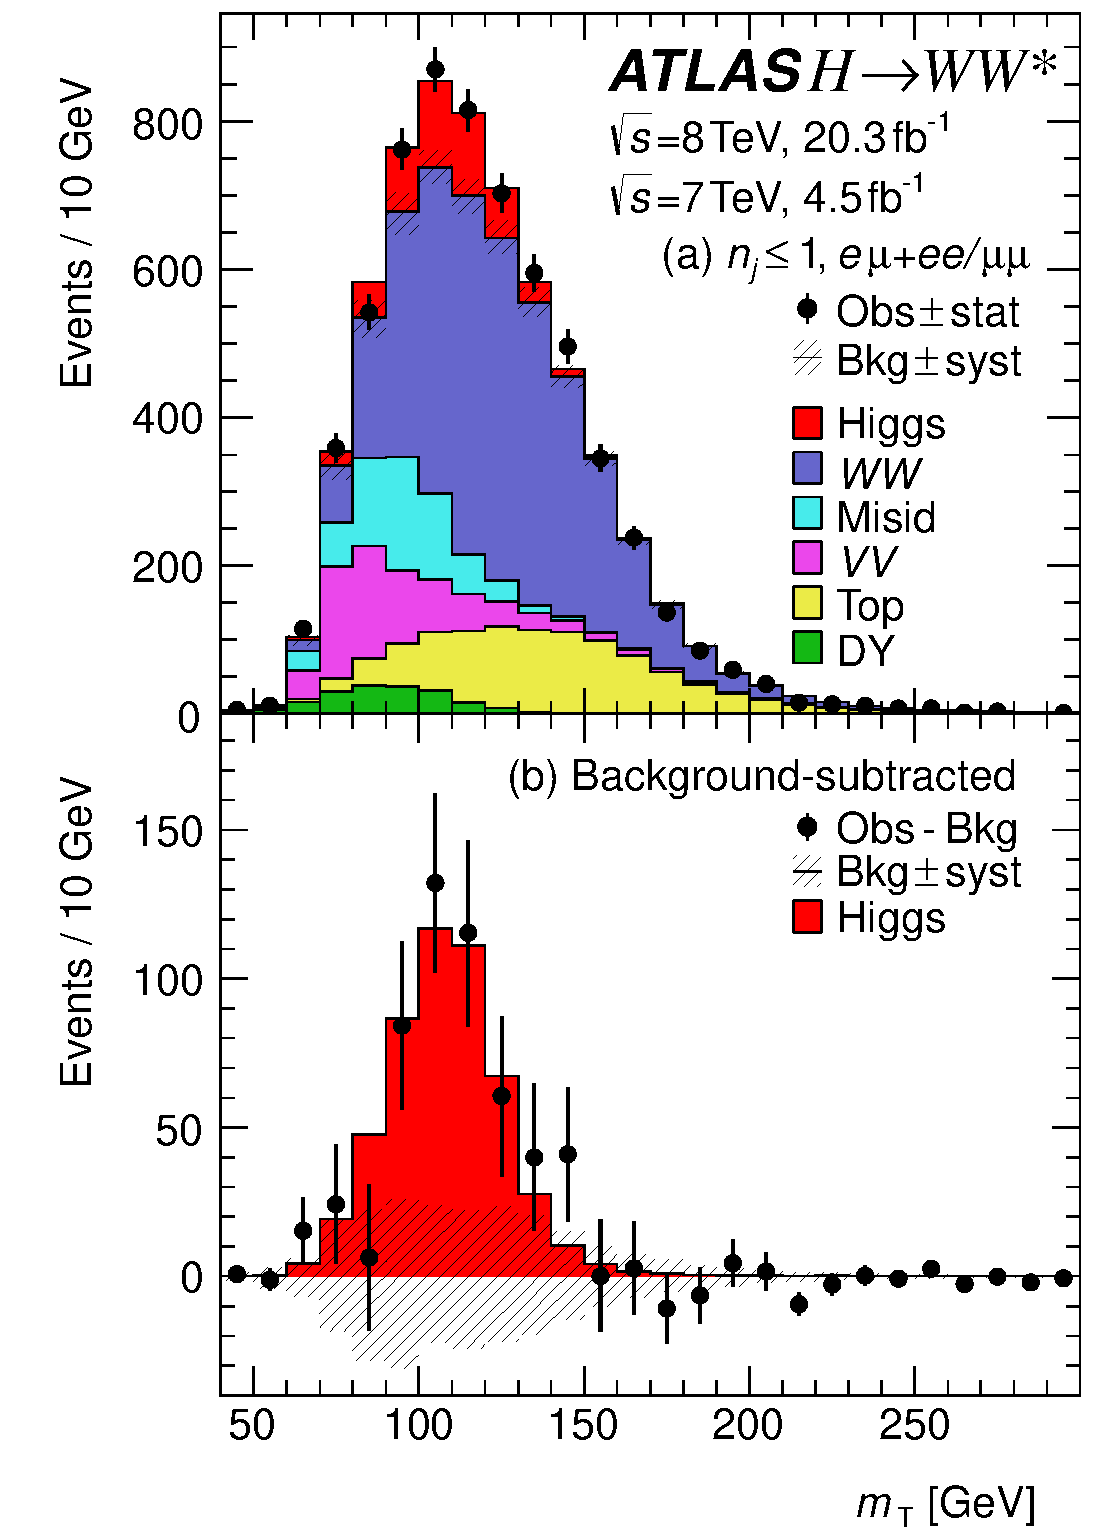
\includegraphics[width=0.32\textwidth]{figures/HIGG-2013-13/fig_35}
  \caption{Discovery plots for the $\Hyy$ (left)~\cite{HIGG-2013-08}, $\HZZ$ (center)~\cite{HIGG-2013-21}, and $\HWW$ (right)~\cite{HIGG-2013-13} analyses.}
  \label{fig:strategy-higgs-yyzzww}
\end{figure}

Pairs of gauge bosons like $\gamma, W, Z$ are produced infrequently at the LHC, hence all three bosonic analyses best measure the ggF Higgs production mechanism since it is has the highest cross section. Their best discriminating variable is typically the reconstructed Higgs mass because there are no significant resonant backgrounds. This can be fully reconstructed in the $\Hyy$ and $\HZZ$ analyses because there are no neutrinos in the decays. In the $\HWW$, the Higgs mass can be partially reconstructed by incorporating the $\MET$ in a transverse mass $m_T$.

\subsubsection{$\Hfermions$}

With the full Run-I dataset and evolving analysis techniques, the searches for fermionic decays of the Higgs boson become competitive in sensitivity with analyses of the bosonic decays. Among these searches, the $\Htautau$ and $\Hbb$ analyses are the most powerful with the Run-I dataset. The $\Htautau$ analysis is described here, especially in the $\tautaulh$ final state. The $\Hbb$ analysis is described in detail elsewhere~\cite{HIGG-2013-23}.

%% The $\Hbb$ analysis employs MVA analysis techniques to search for the $VH$ production mechanism, where $V$ is a vector boson that can decay like $\Wlv$, $\Zll$, or $\Zvv$. This production mode is chosen because $b$-quarks are frequently produced at hadron colliders, and searching only for two $b$-jets is prohibitive. Events with two $b$-jets produced in association with a vector boson provide a more optimal tag.

%% \begin{figure}[tp]
%%   \centering
%%   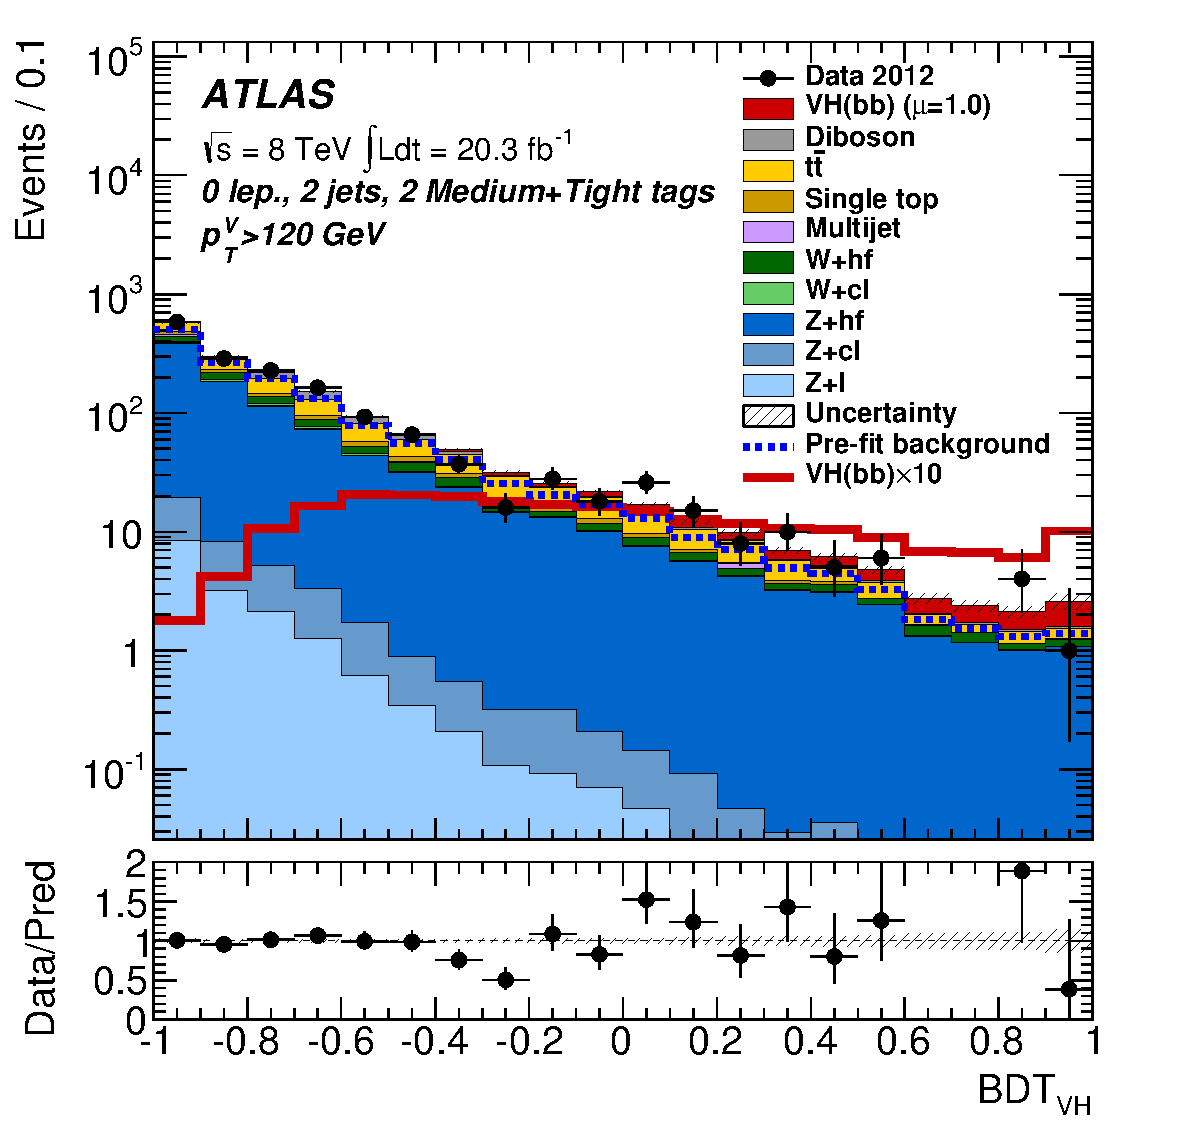
\includegraphics[width=0.32\textwidth]{figures/HIGG-2013-23/fig_11a}
%%   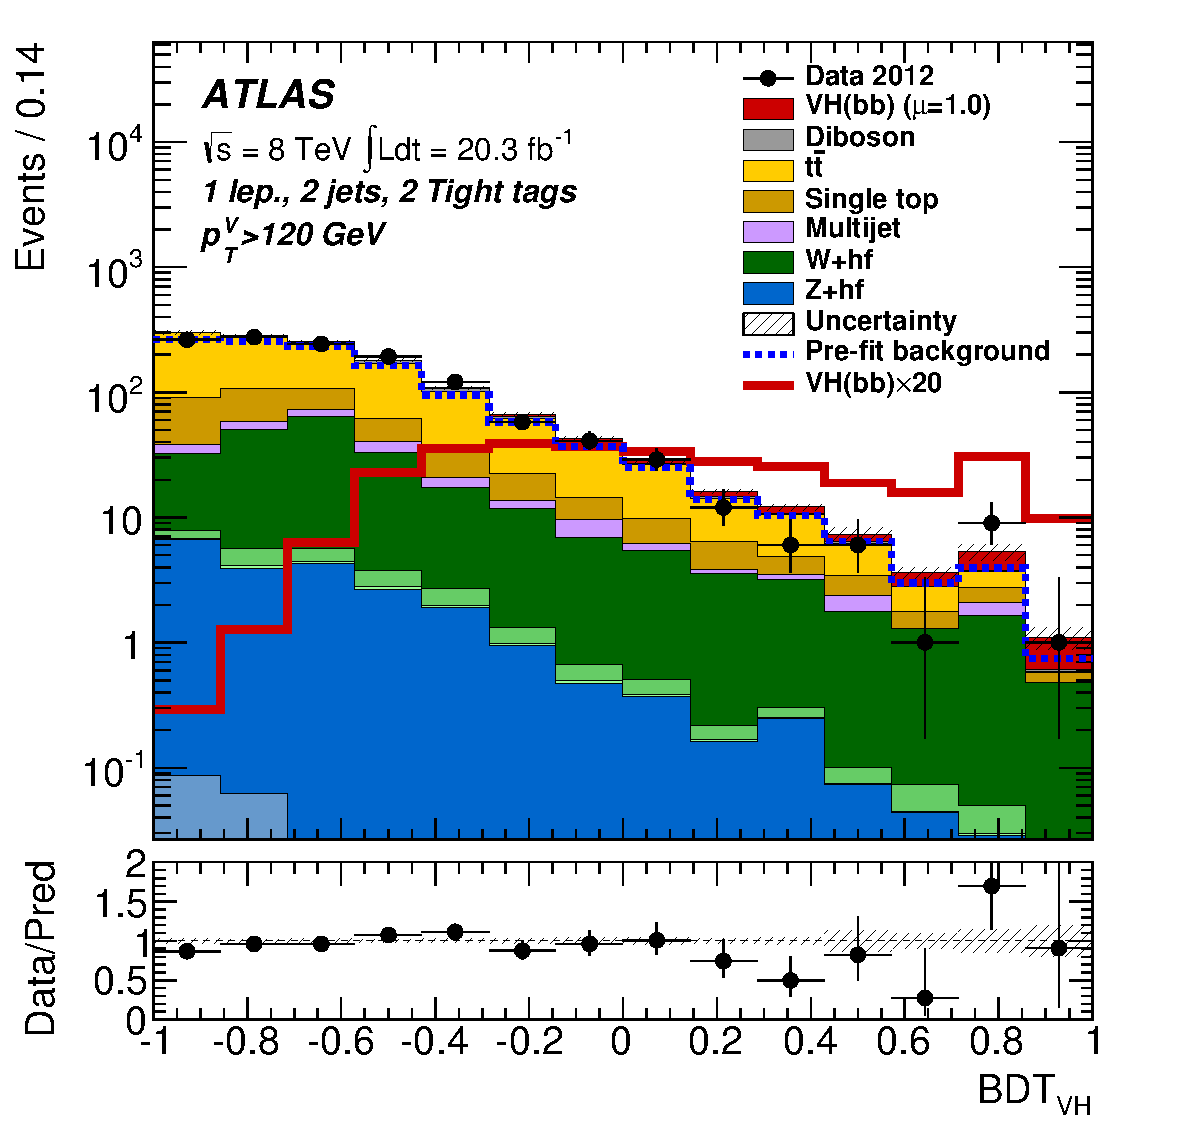
\includegraphics[width=0.32\textwidth]{figures/HIGG-2013-23/fig_12c}
%%   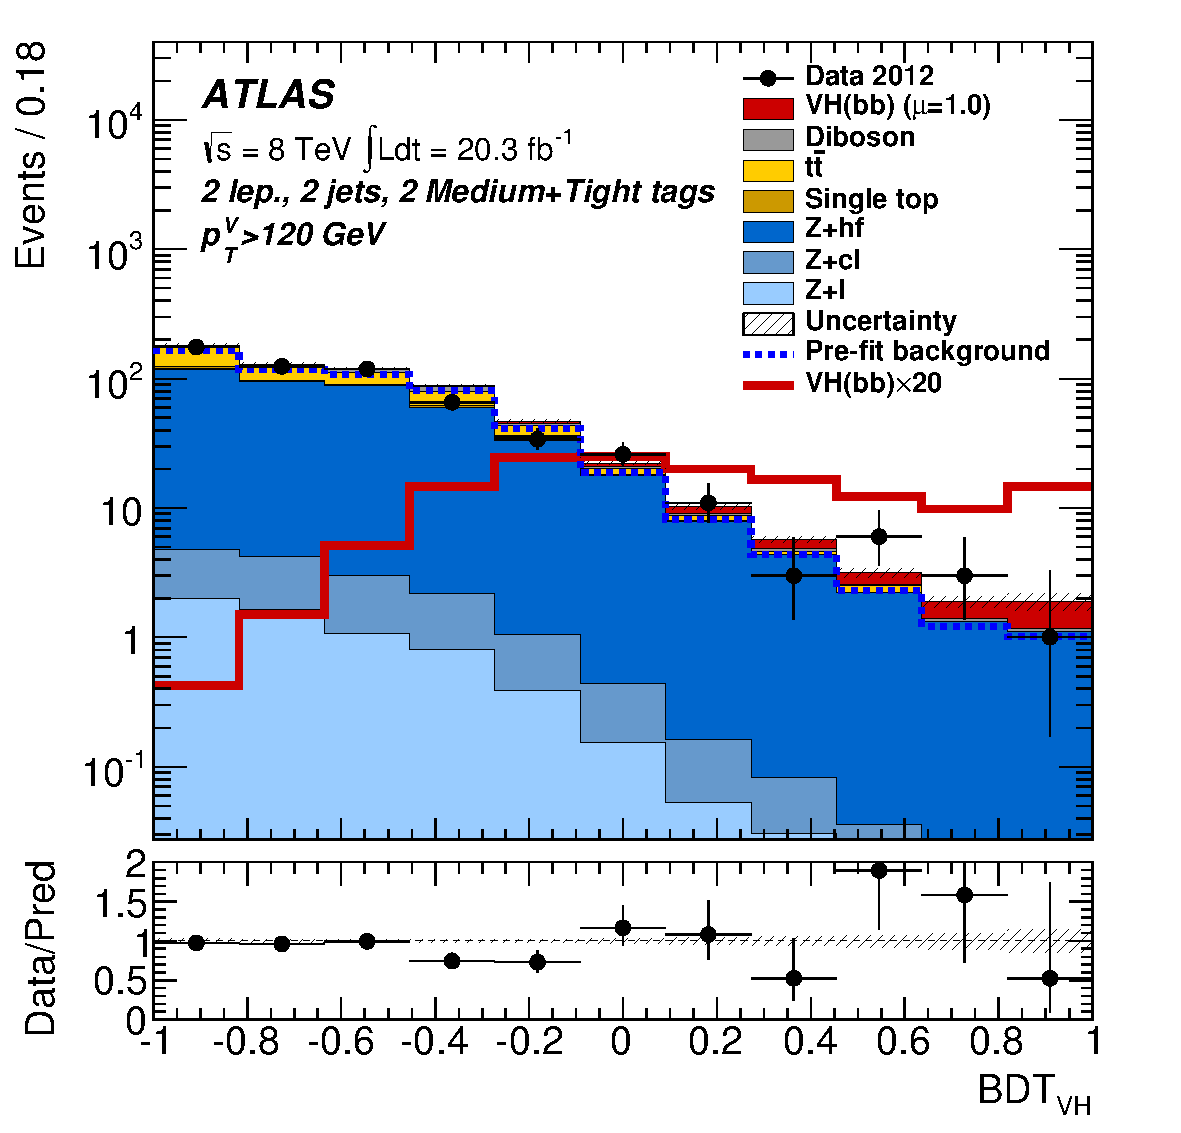
\includegraphics[width=0.32\textwidth]{figures/HIGG-2013-23/fig_13b}
%%   \caption{Data and predicted signal and backgrounds in the $V\!\Hbb$ BDT analysis in the 0-lepton (left), 1-lepton (center), and 2-lepton (right) analyses~\cite{HIGG-2013-23}.}
%%   \label{fig:strategy-higgs-vhbb}
%% \end{figure}

\subsection{$\Htautau$}
\label{sec:strategy-htautau}

The $\Htautau$ analysis is naturally broken into three final states (or ``channels'') given the combinatorics of tau lepton decays: $\tautaulh$, $\tautauhh$, and $\tautaull$. Their branching fractions are shown in \cref{fig:strategy-decaypie}. The experimental methods of each final state are conceptually similar though not identical. This thesis describes the $\Htautaulh$ in detail since it was the focus of the author, and the $\Htautauhh$ and $\Htautaull$ are only briefly summarized.

\begin{figure}[tp]
  \centering
  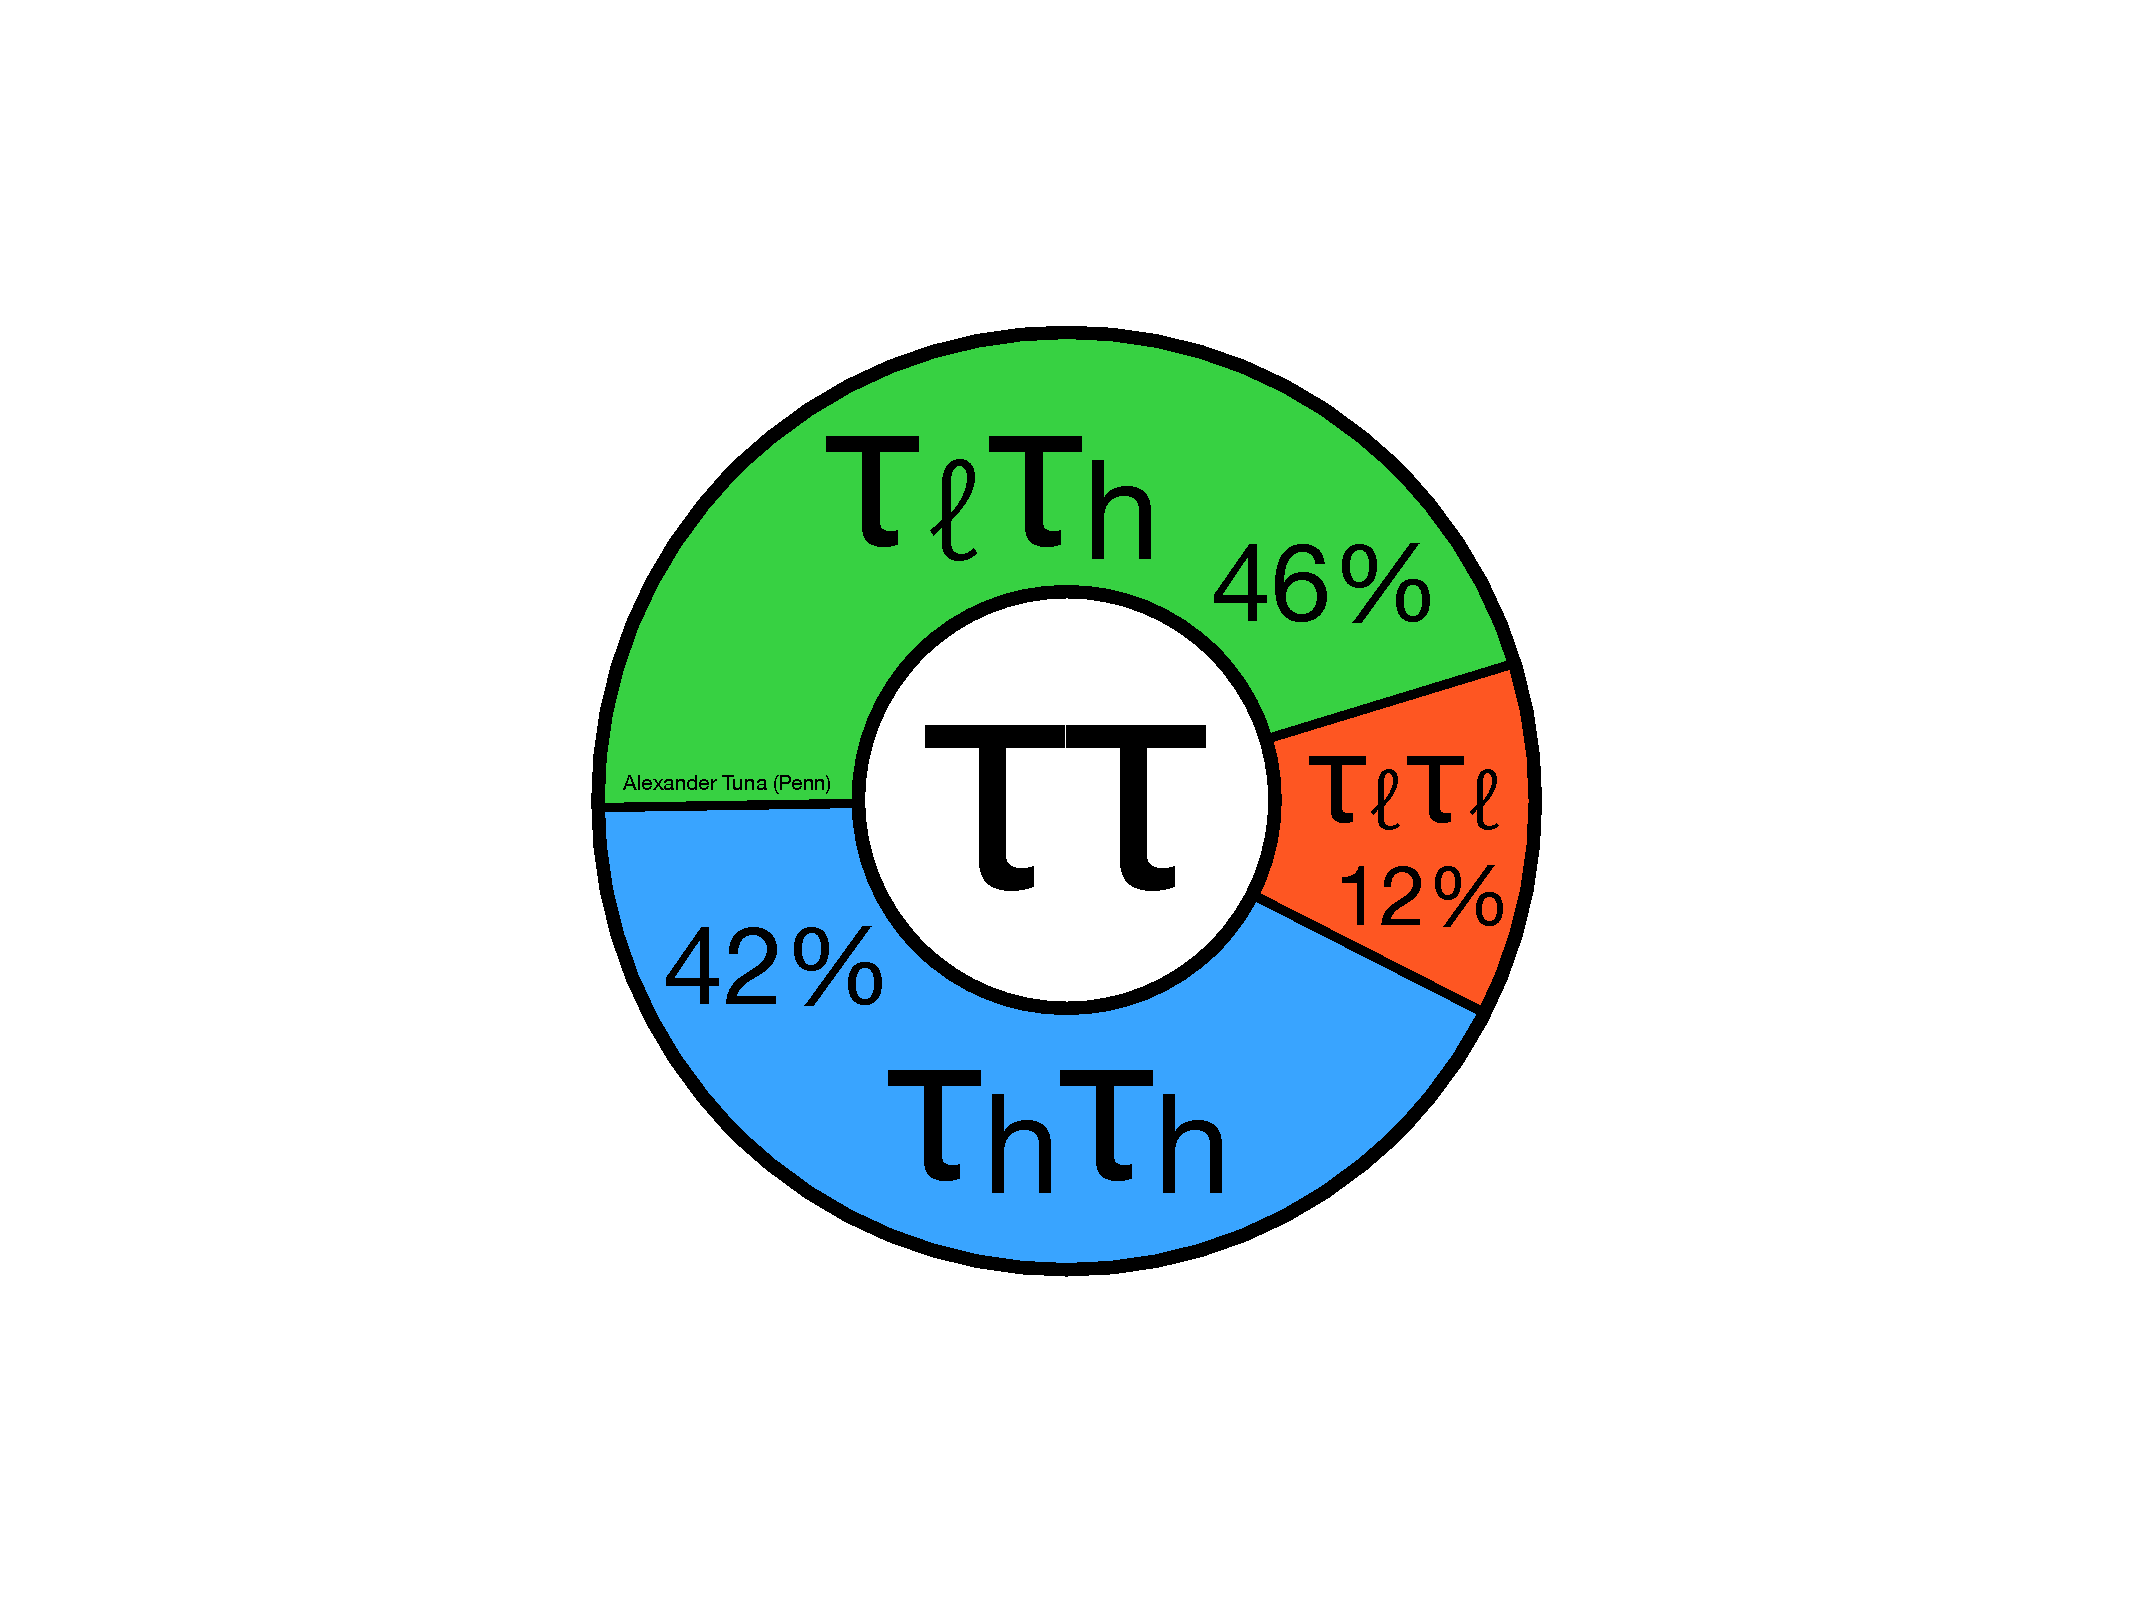
\includegraphics[width=0.48\textwidth]{figures/piecharts/tautaudecay}
  \caption{Pie chart of di-tau lepton decay branching fractions.}
  \label{fig:strategy-decaypie}
\end{figure}

Unlike the $\Hbosons$ analyses, the $\Htautau$ suffers from a large background of $\Ztautau$. This background cannot be easily disentangled from $\Htautau$ because multiple neutrinos exist in the decays of the tau leptons and $\mtautau$ cannot be fully reconstructed. The cross-section for QCD production for $\Ztautau$ is also $10^3$ times larger than ggF $\Htautau$ production~\cite{HIGG-2013-32}, which is the largest production mode.

The cross-section for EW production of $\Ztautau$, however, is only $4$ times larger than VBF $\Htautau$ production~\cite{HIGG-2013-32}, which is the second largest production mode and can be tagged via the associated VBF jets. This makes the $\Htautau$ analysis a natural candidate for \textit{categorization}, where Higgs production modes are targeted with much smaller cross sections than the inclusive production but with better experimental sensitivity.

\section{Triggers}
\label{sec:strategy-triggers}

The lowest unprescaled single lepton triggers, as described in \cref{sec:trigger}, are used for the $\Htautaulh$ data sample. These correspond to offline lepton $\pt$ thresholds of 26 GeV in the 8 TeV dataset. $\LTT$ triggers are considered to recover data events with leptons below the single lepton trigger thresholds, but they are ultimately not used due to lack of sensitivity and additional complications. The triggers used are shown in \cref{tab:strategy-triggers}.

\begin{table}[bp]
  \centering
  \renewcommand{\arraystretch}{1.4}
  \caption{Triggers used in the 8 TeV $\Htautaulh$ analysis.}
  \begin{tabular}{c|c|c}
  channel      & L1              & HLT                      \\
  \hline
  $\Htautaueh$ & \texttt{EM18VH} & \texttt{e24vhi\_medium1} \\
  $\Htautaumh$ & \texttt{MU20}   & \texttt{mu24i\_tight}    \\
\end{tabular}

  \label{tab:strategy-triggers}
\end{table}

\section{Physics objects}
\label{sec:strategy-objects}

\subsection{Electrons, muons, and $\tauh$}
\label{sec:strategy-leptons}

Electrons, muons, and $\tauh$ are selected according to the reconstruction, identification, and calibration algorithms described in \cref{sec:particles,sec:taus-hadrons}. The selection criteria used are summarized in \cref{tab:strategy-objects-emutau}.

\begin{table}[bp]
  \centering
  \renewcommand{\arraystretch}{1.4}
  \caption{Lepton and $\tauh$ criteria used in the 8 TeV $\Htautaulh$ analysis.}
  \begin{tabular}{c|c}
  object   & criteria \\
  \hline\hline
  \multirow{2}{*}{Electrons} & $\pt >$ 26 GeV, $|\eta| < 2.47$ (excl. crack) \\
                             & \texttt{tightPP}, $f_\text{isol.}^\text{track} < 0.06$, $f_\text{isol.}^\text{calo.} < 0.06$ \\
  \hline
  \multirow{2}{*}{Muons}     & $\pt >$ 26 GeV, $|\eta| < 2.5$ \\
                             & \texttt{isCombined}, $f_\text{isol.}^\text{track} < 0.06$, $f_\text{isol.}^\text{calo.} < 0.06$ \\
  \hline
  \multirow{3}{*}{$\tauh$}   & $\pt >$ 20 GeV, $|\eta| < 2.47$, $|\eta^\text{lead track}| < 2.47$ \\
                             & \texttt{JetBDTSigMedium}, no overlap with reco. muon or \texttt{loosePP} electron \\
                             & \texttt{EleBDTMedium} in $\tautaueh$ channel \\
\end{tabular}

  \label{tab:strategy-objects-emutau}
\end{table}

Electrons are required to have $\pt >$ 26 GeV and pass the \texttt{tightPP} identification algorithm and be isolated both in the tracker and the calorimeter. Less than 6\% of the magnitude of the electron energy is required to exist in an isolation cone of 0.4 in the tracker and 0.2 in the calorimeter. The recent electron likelihood identification algorithm~\cite{ATLAS-CONF-2014-032} is explored, and though improvement is observed, time constraints prevent its use in this analysis.

Muons are required to have $\pt >$ 26 GeV and to satisfy the \texttt{isCombined} reconstruction algorithm and be isolated both in the tracker and the calorimeter. Less than 6\% of the magnitude of the muon energy is required to exist in an isolation cone of 0.4 in the tracker and 0.2 in the calorimeter.

$\tauh$ are required to have $\pt >$ 20 GeV and to pass the \texttt{JetBDTSigMedium} jet discriminator. As discussed in \cref{sec:taus-hadrons}, this identification algorithm includes isolation criteria. $\tauh$ are also required to not overlap with any reconstructed muon candidates or \texttt{loosePP} electron candidates, as discussed in \cref{sec:taus-leptonfakes}. In the $\tautaueh$ final state, $\tauh$ are additionally required to pass the \texttt{EleBDTMedium} electron discriminator.

For the purpose of vetoing events with additional light leptons, $\pt$ and identification criteria for electrons (muons) are relaxed to 15 GeV (10 GeV) and \texttt{loosePP} (\texttt{loose}), respectively.

\subsection{Jets and $\MET$}
\label{sec:strategy-hadronic}

Jets, $b$-jets, and $\MET$ are selected according to the reconstruction, identification, and calibration algorithms described in \cref{sec:particles}. The selection criteria used are summarized in \cref{tab:strategy-objects-jetmet}.

\begin{table}[bp]
  \centering
  \renewcommand{\arraystretch}{1.4}
  \caption{Jet, $b$-jet, and $\MET$ criteria used in the 8 TeV $\Htautaulh$ analysis.}
  \begin{tabular}{c|c}
  object   & criteria \\
  \hline\hline
  \multirow{2}{*}{Jets}     & $\pt >$ 30 GeV, $|\eta| < 4.5$ \\
                            & $\text{JVF} > 0.5$ if $|\eta| < 2.4$ \\
  \hline
  \multirow{2}{*}{$b$-jets} & $\pt >$ 30 GeV, $|\eta| < 2.4$ \\
                            & 70\% \texttt{MV1} $b$-tag working point\\
  \hline
  \multirow{2}{*}{$\MET$}   & hard term consistent with object selection (ignoring photons) \\
                            & STVF soft term \\
\end{tabular}

  \label{tab:strategy-objects-jetmet}
\end{table}

Jets are required to have $\pt >$ 30 GeV and pass a requirement of $\text{JVF} > 0.5$ if they are within the tracking volume $\eta(\text{jet}) < 2.4$. Jets are disambiguated from other physics objects by removing the jet if it overlaps with any electron, muon, or $\tauh$ passing identification requirements previously discussed. Jets are classified as $b$-jets if they are within the tracking volume and pass the 70\% working point of the \texttt{MV1} $b$-tagging algorithm.

$\MET$ is calculated with hard objects as selected by the analysis thresholds and with a soft term from the STVF method, as described in \cref{sec:neutrinos}. No explicit cuts on the $\MET$ are made at any stage of the $\tautaulh$ analysis because the $\MET$ spectra for $\Htautau$ does not strongly discriminate the dominant backgrounds, $\Ztautau$ and $\Wjets$, which have neutrinos in the final state. A track-based soft term is explored, and though improvement is observed, time constraints prevent its use in this analysis.

\section{Categorization}
\label{sec:strategy-categorization}

Event selection is done in two stages: pre-selection and categorization. The first step, pre-selection, is meant to be a simple and pared down event selection on top of which further selections are built. The second step, categorization, adds additional selection to the pre-selection for defining signal regions. A cartoon of the pre-selection and categorizations are shown in \cref{fig:strategy-category-cartoons}.

\begin{figure}[tp]
  \centering
  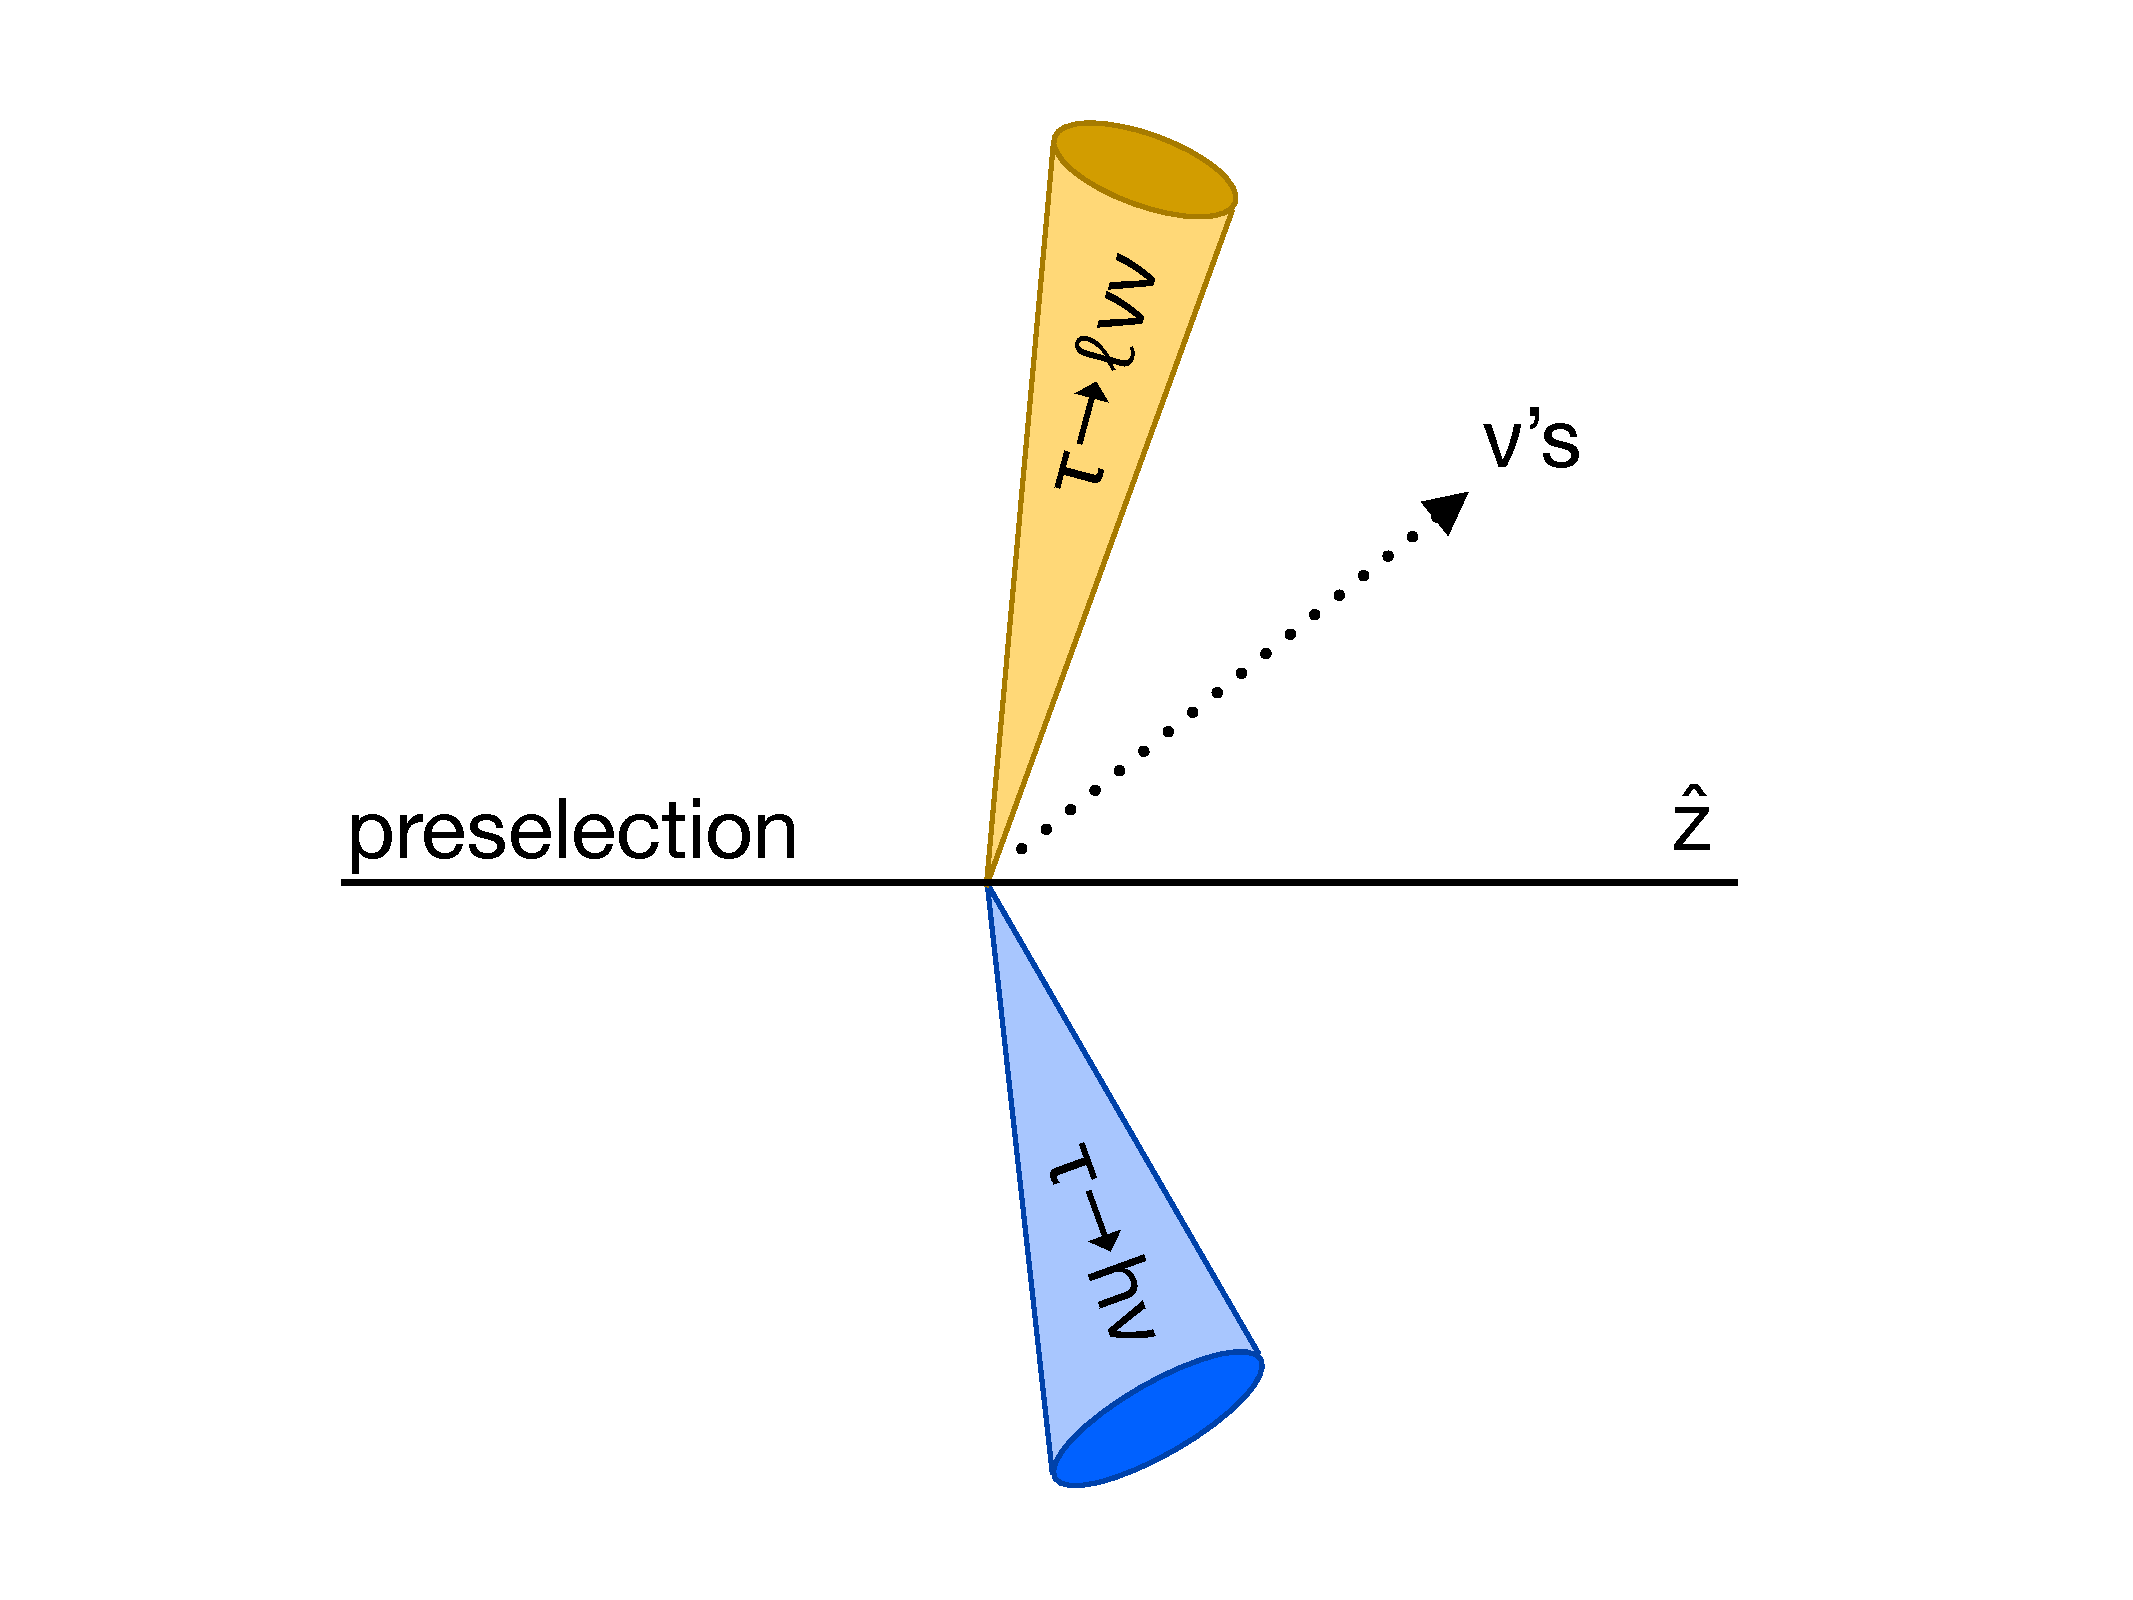
\includegraphics[width=0.48\textwidth]{figures/category-cartoons/presel}
  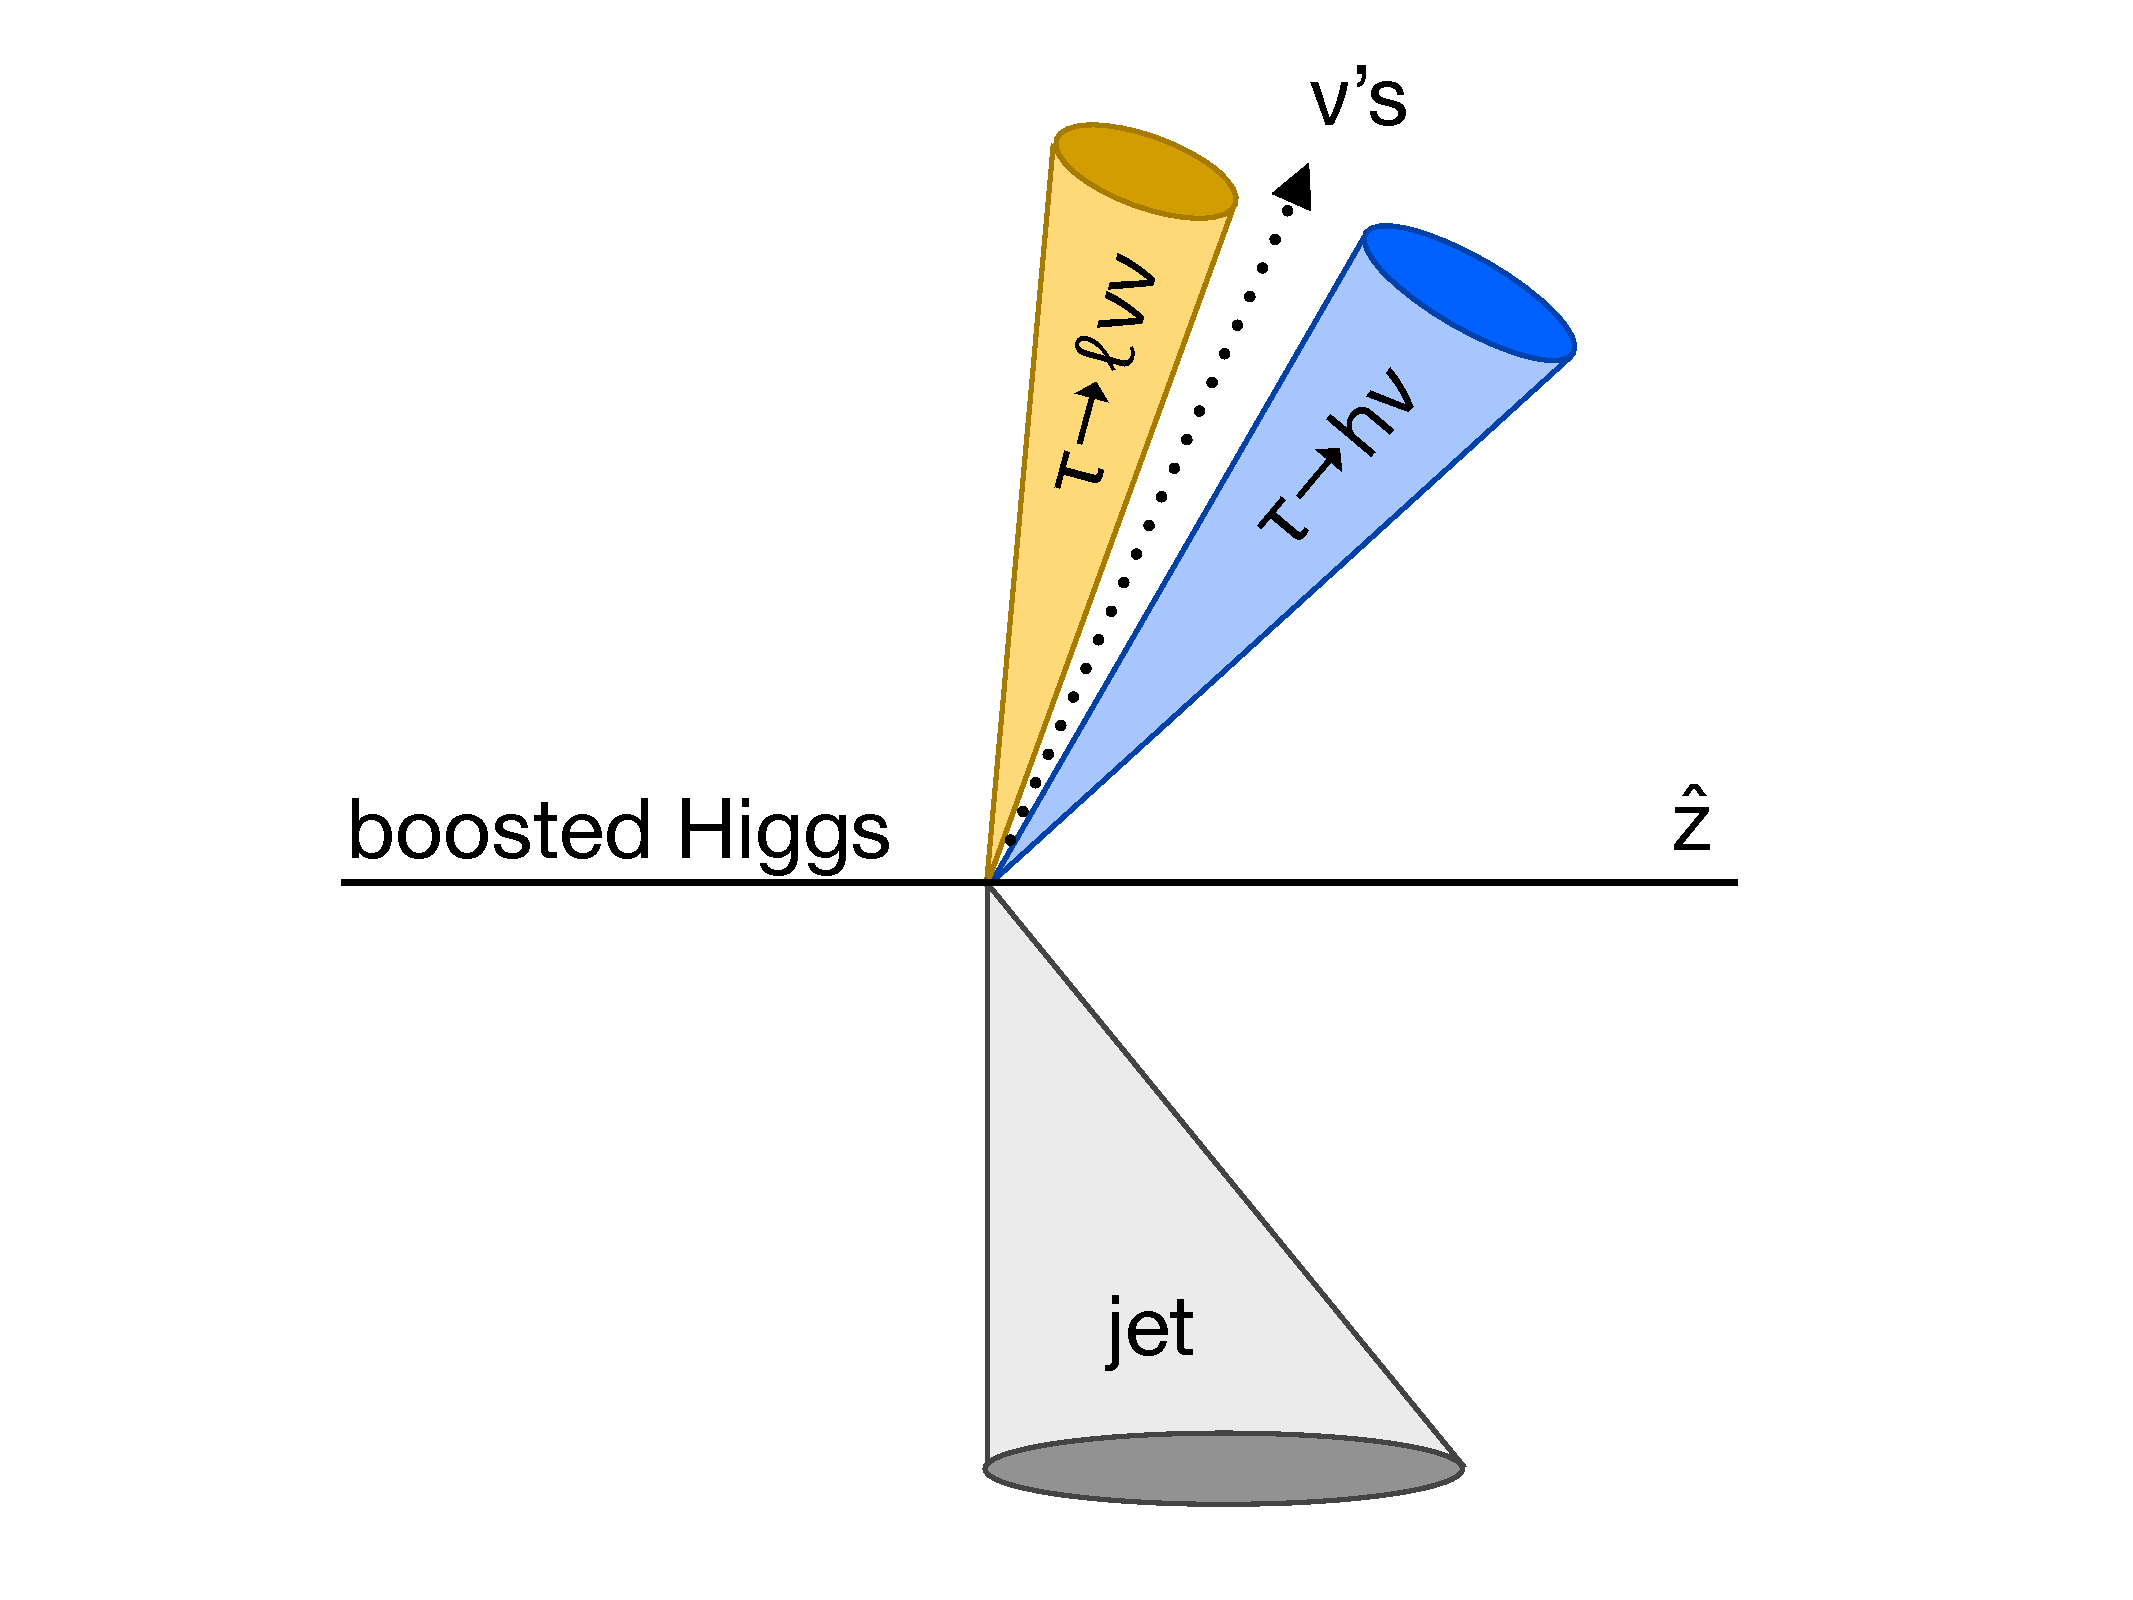
\includegraphics[width=0.48\textwidth]{figures/category-cartoons/boost}
  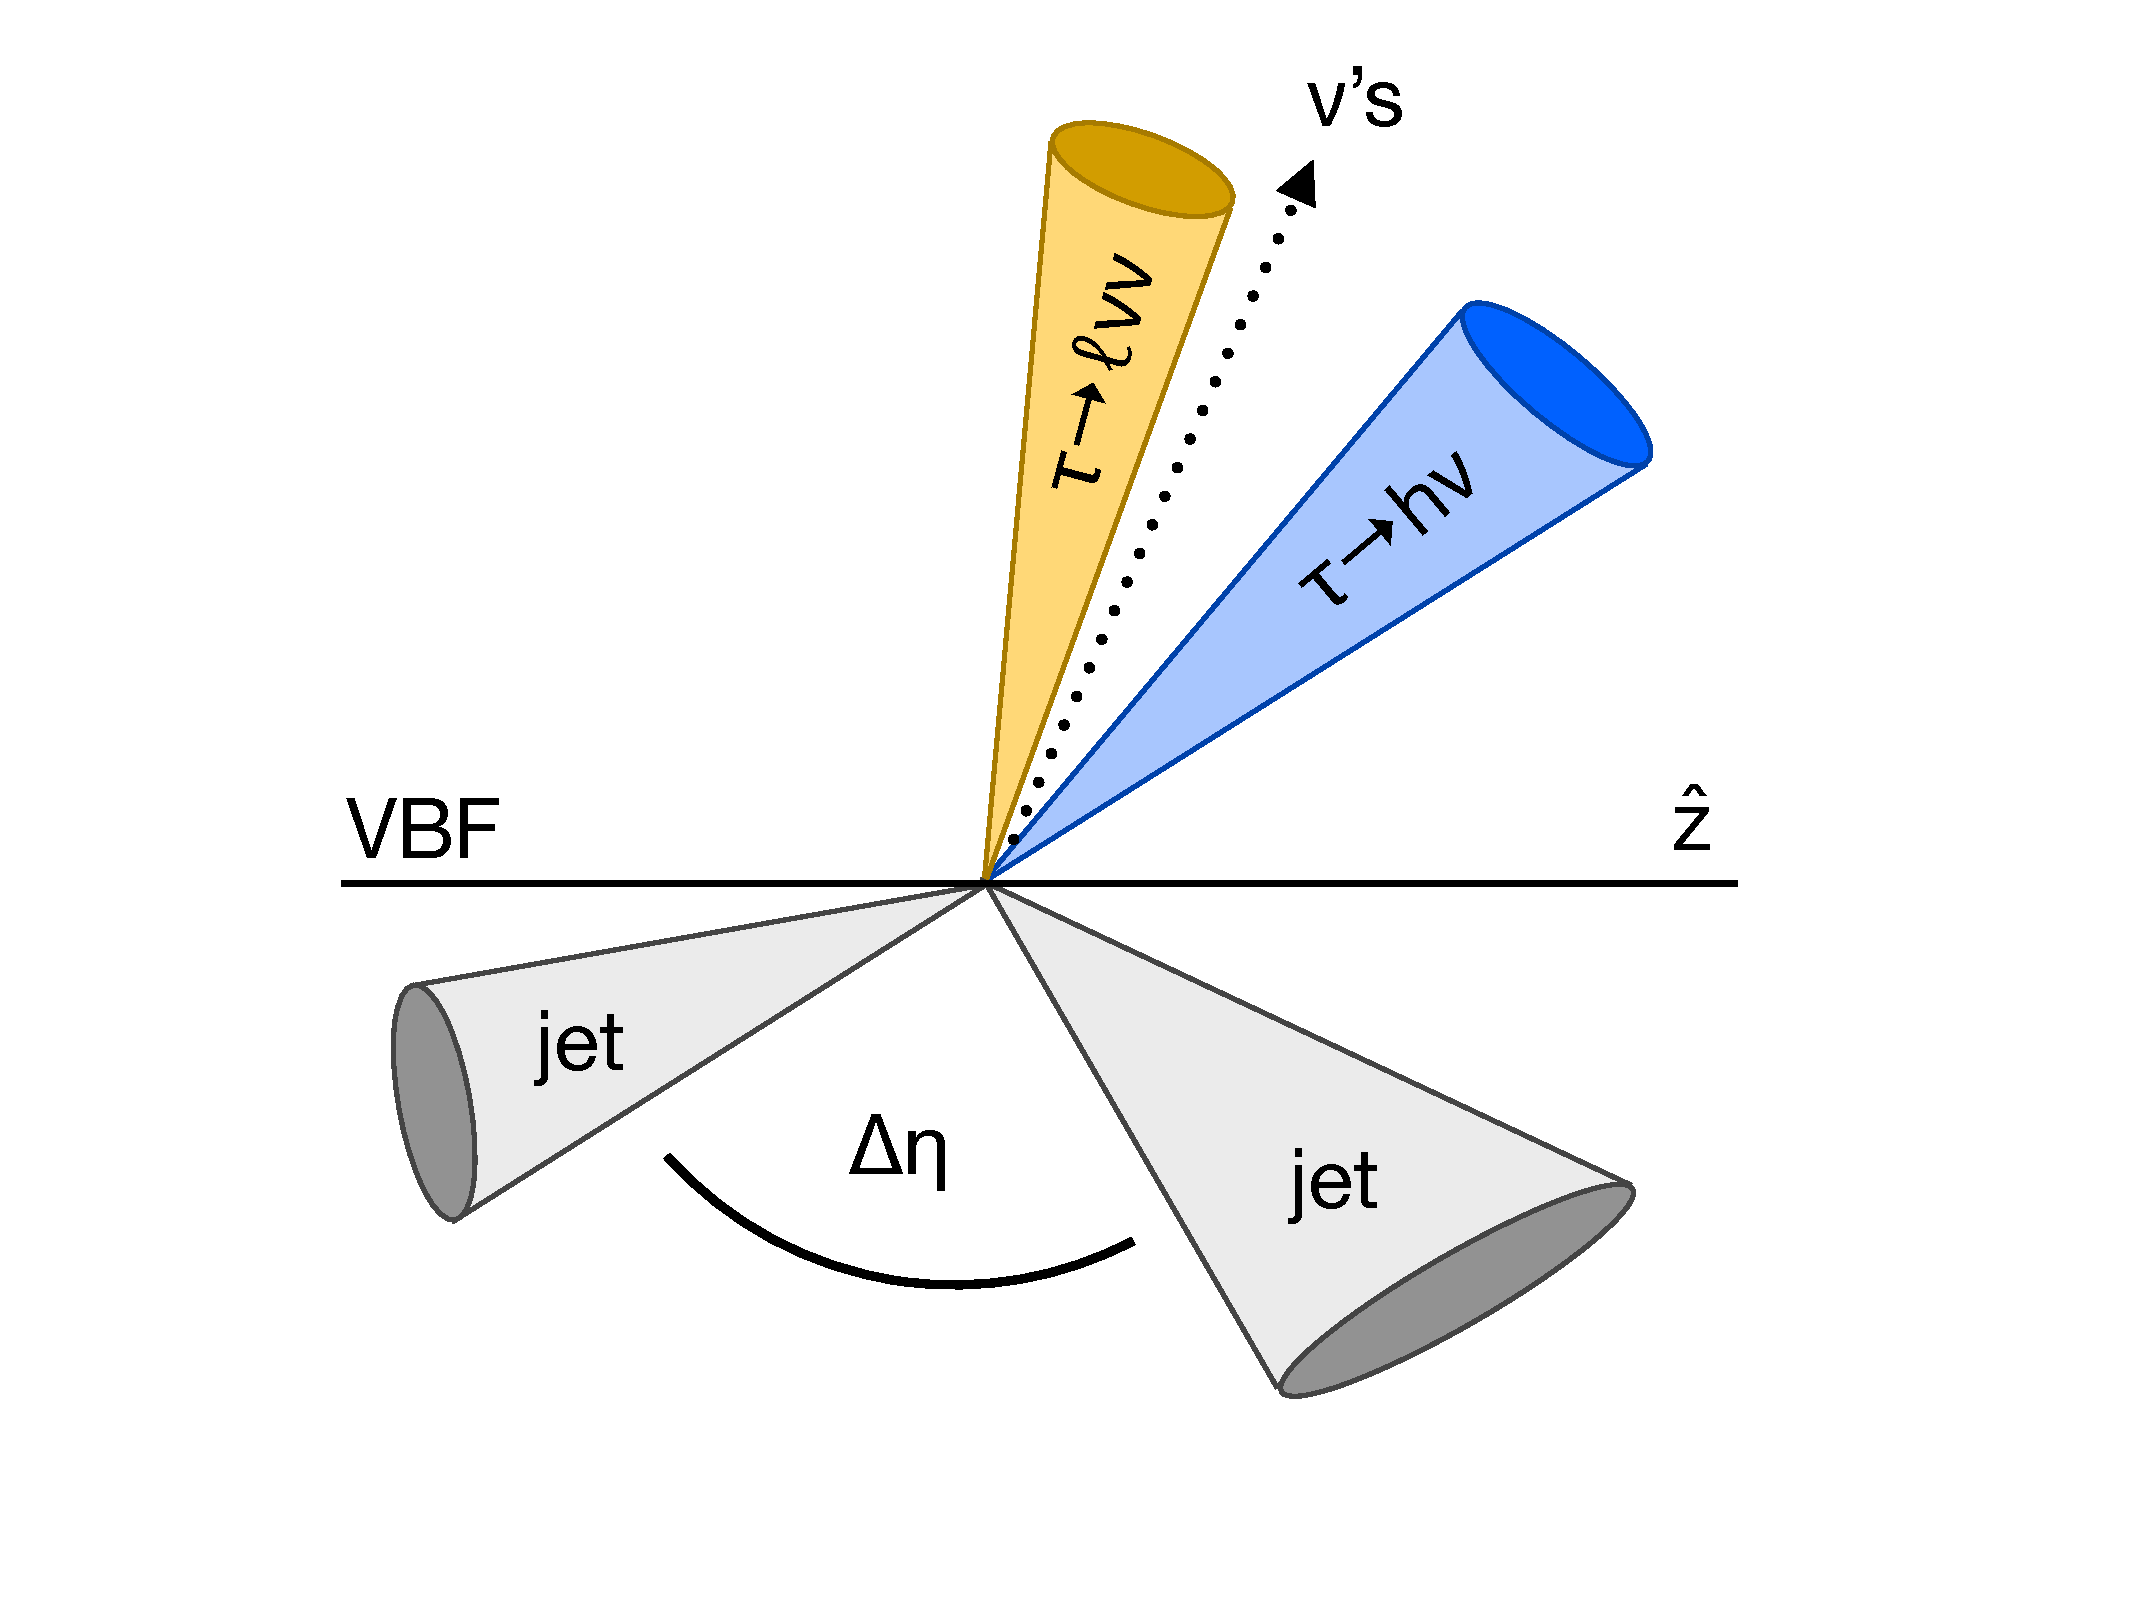
\includegraphics[width=0.48\textwidth]{figures/category-cartoons/vbf}
  \caption{Cartoon depiction of the relevant categories in the $\Htautaulh$ analysis: pre-selection, boosted, and VBF.}
  \label{fig:strategy-category-cartoons}
\end{figure}

\subsection{Pre-selection}
\label{sec:strategy-preselection}

Pre-selection of the $\tautaulh$ analysis requires exactly one light lepton, exactly one $\tauh$, exactly zero $b$-tagged jets, and that the lepton and $\tauh$ have opposite charges. A requirement of $\mT < 70$ GeV is applied, which reconstructs a transverse $W$ mass and is $\approx\!95$\% efficient for $\Htautau$. The pre-selection is summarized in \cref{tab:strategy-selection}.

This simple selection is shared among all signal regions. Individual pieces of the selection can be reversed to define control regions in data rich in $\fakes$. For example, the $\mT$ requirement is reversed to defined a $\Wjets$ control region.

Event kinematics for data and prediction at the pre-selection stage are shown in \cref{fig:stategy-presel-1,fig:stategy-presel-2}. These predictions are discussed in more detail in \cref{chap:backgrounds}. Since the selection is very inclusive, many hundreds of thousands of events pass the pre-selection, especially $\Ztautau$ and $\fakes$.

\clearpage

\begin{figure}[tp]
  \centering
  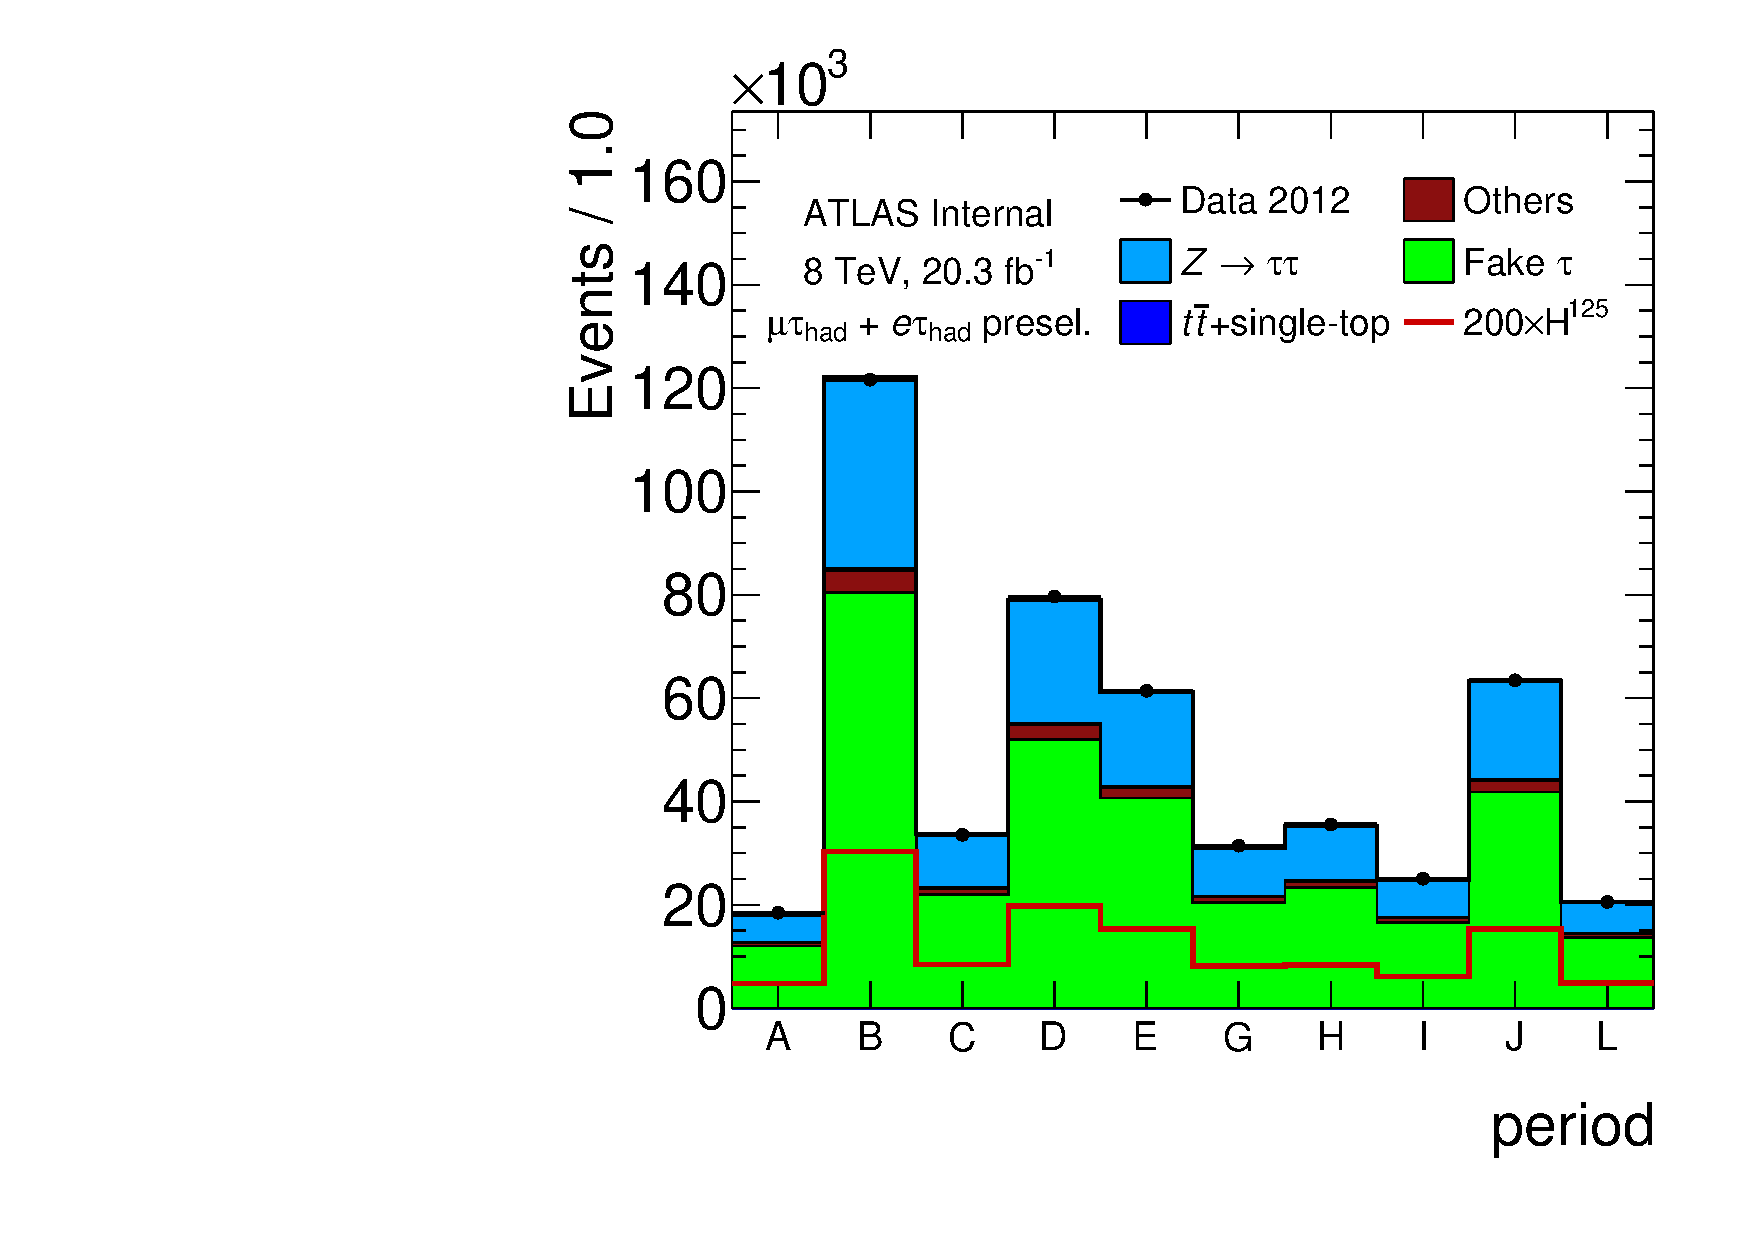
\includegraphics[width=0.32\textwidth]{figures/presel/period}
  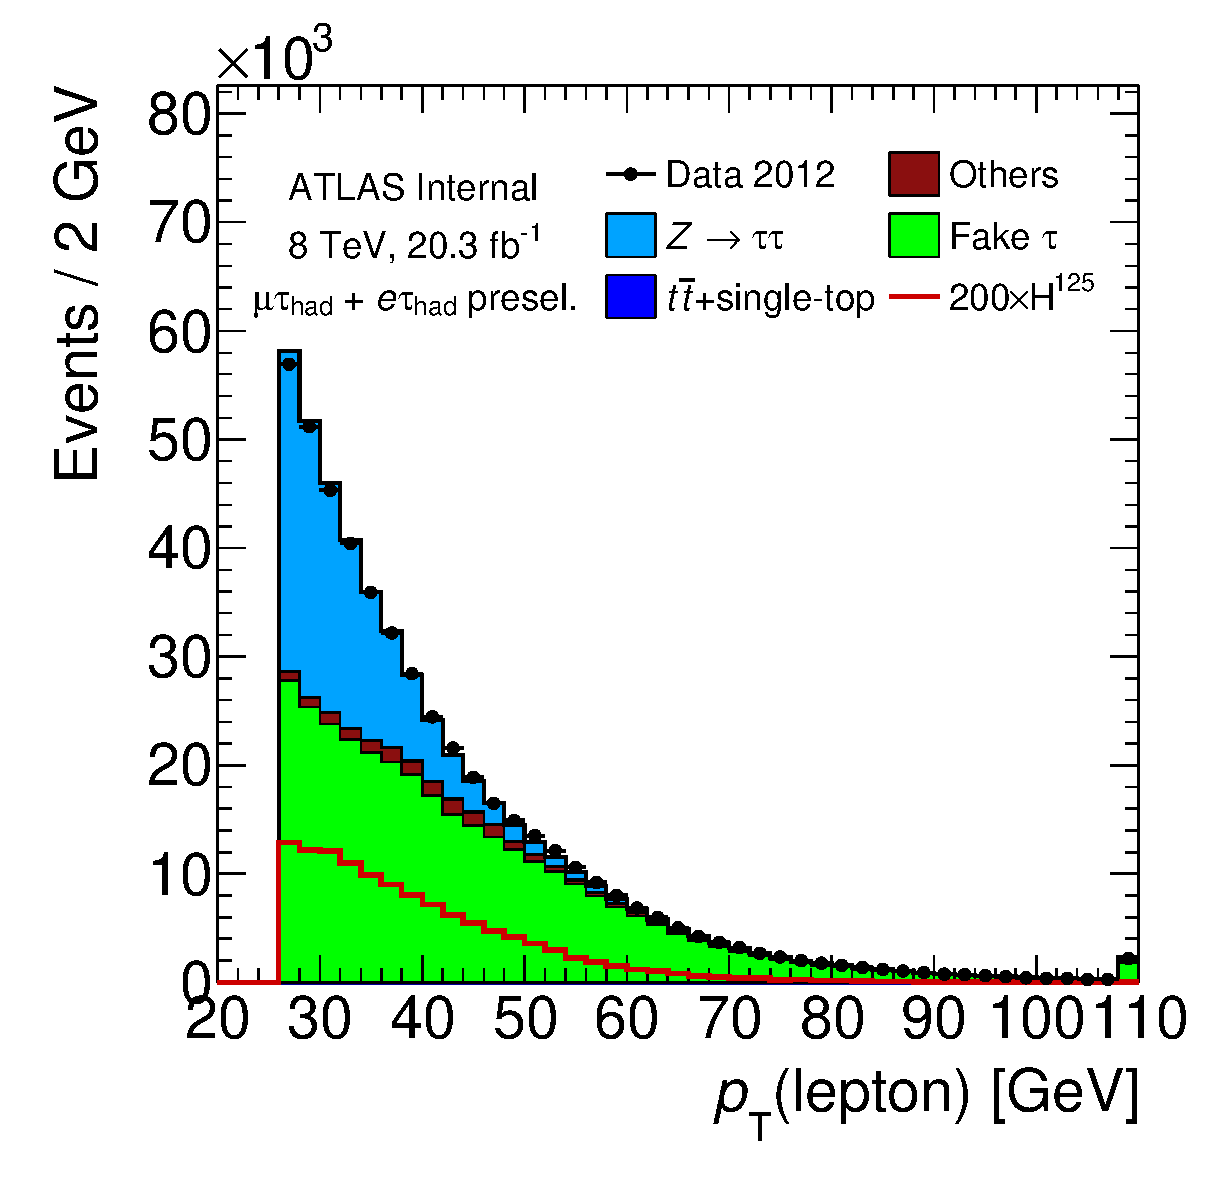
\includegraphics[width=0.32\textwidth]{figures/presel/lep-pt-hi}
  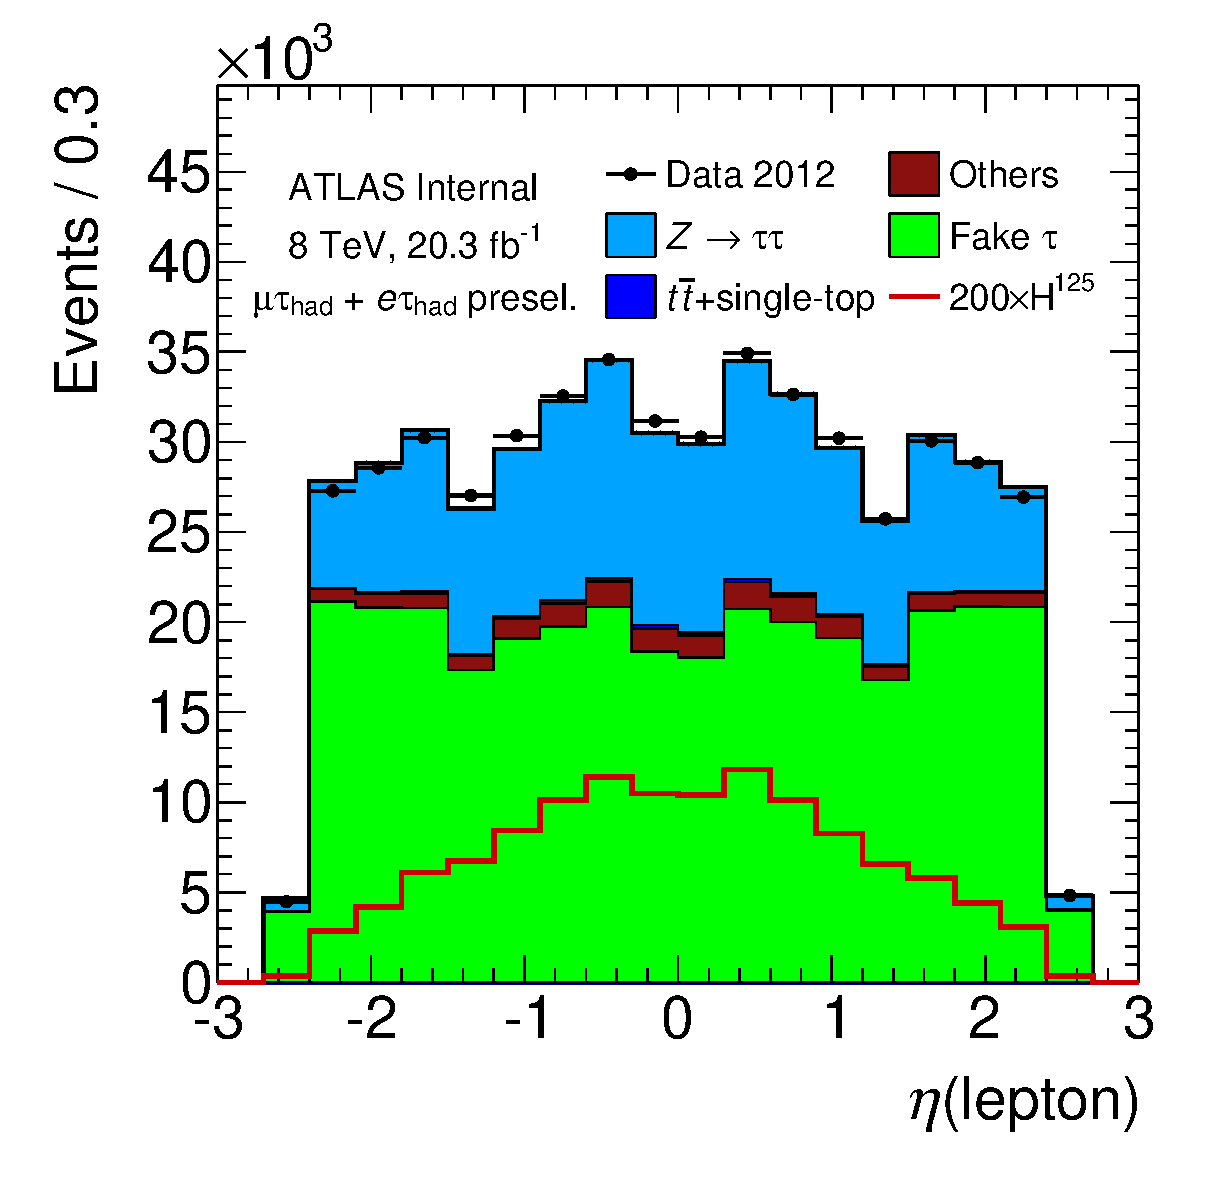
\includegraphics[width=0.32\textwidth]{figures/presel/lep-eta} \\
  % --------------
  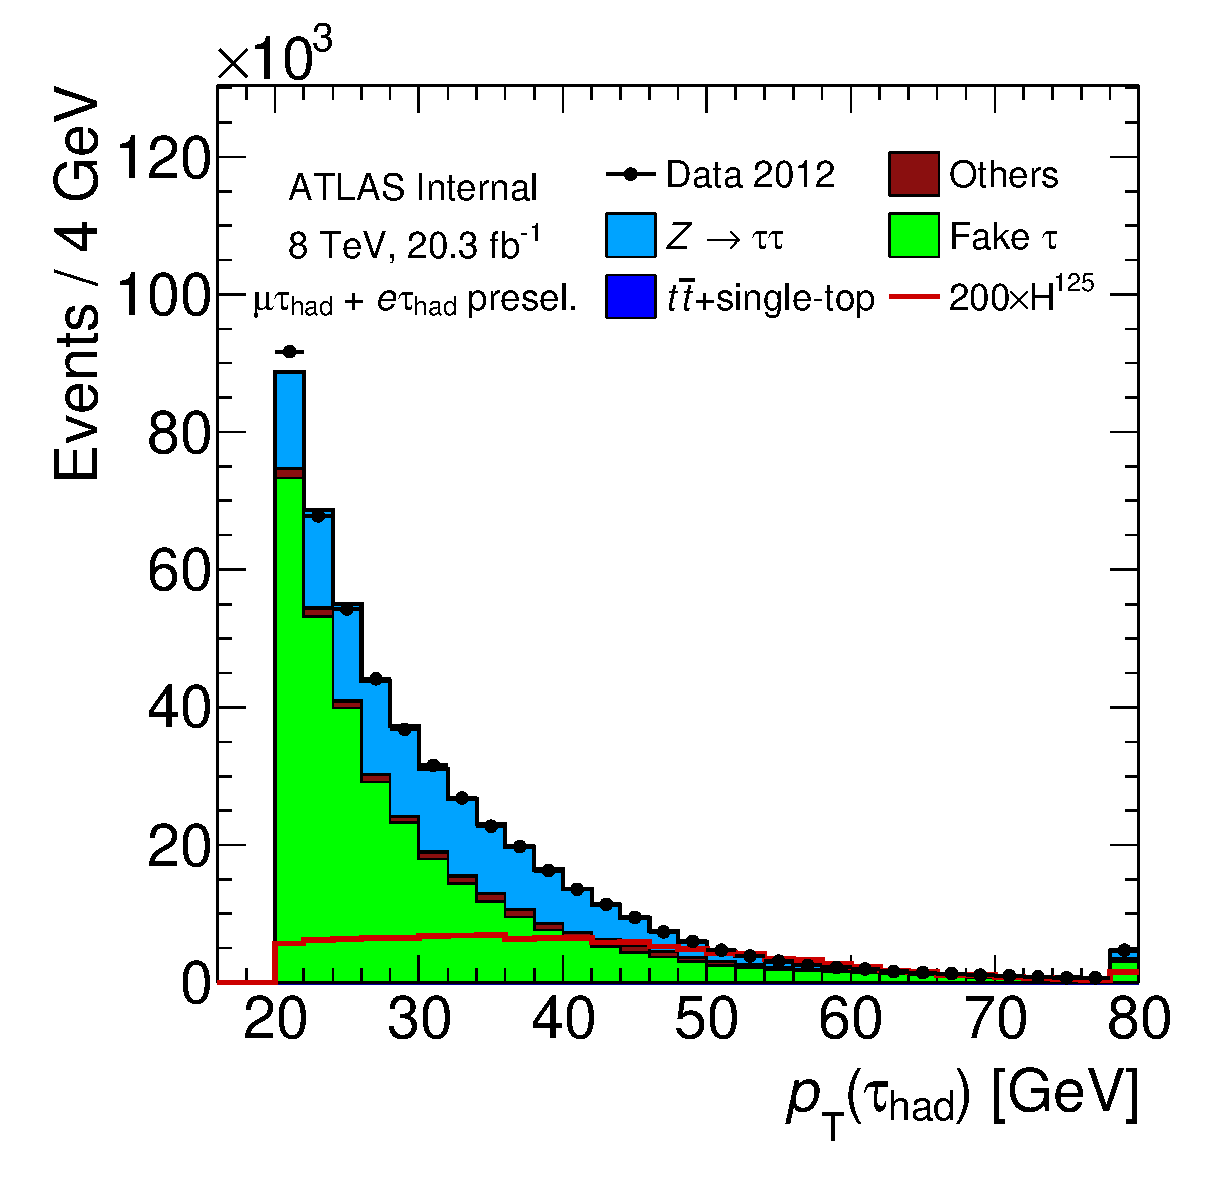
\includegraphics[width=0.32\textwidth]{figures/presel/tau-pt}
  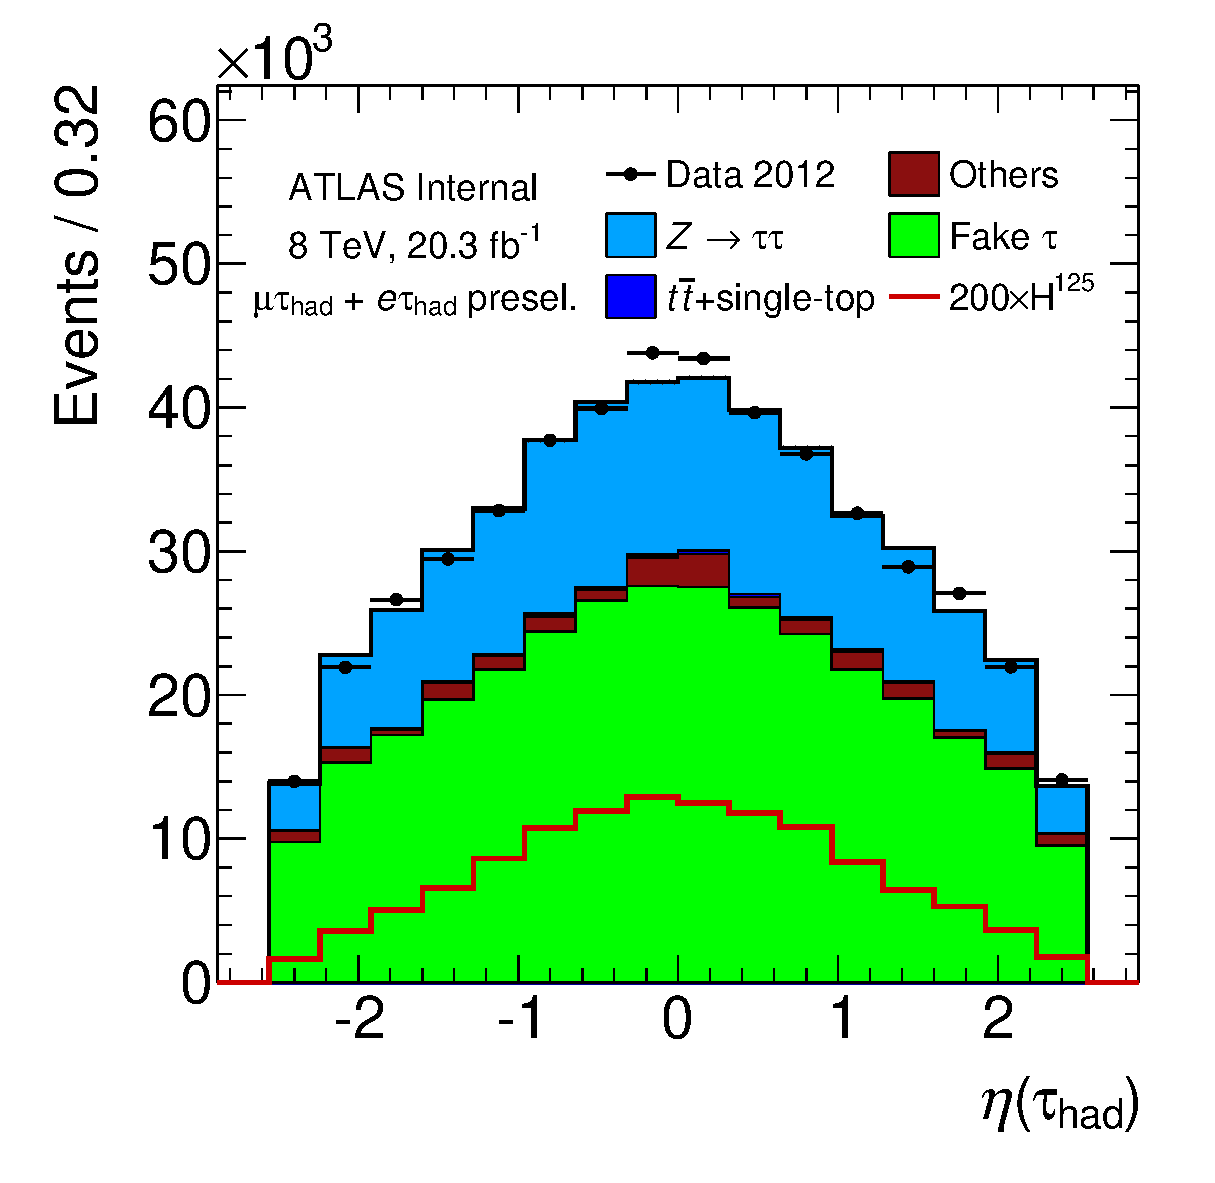
\includegraphics[width=0.32\textwidth]{figures/presel/tau-eta}
  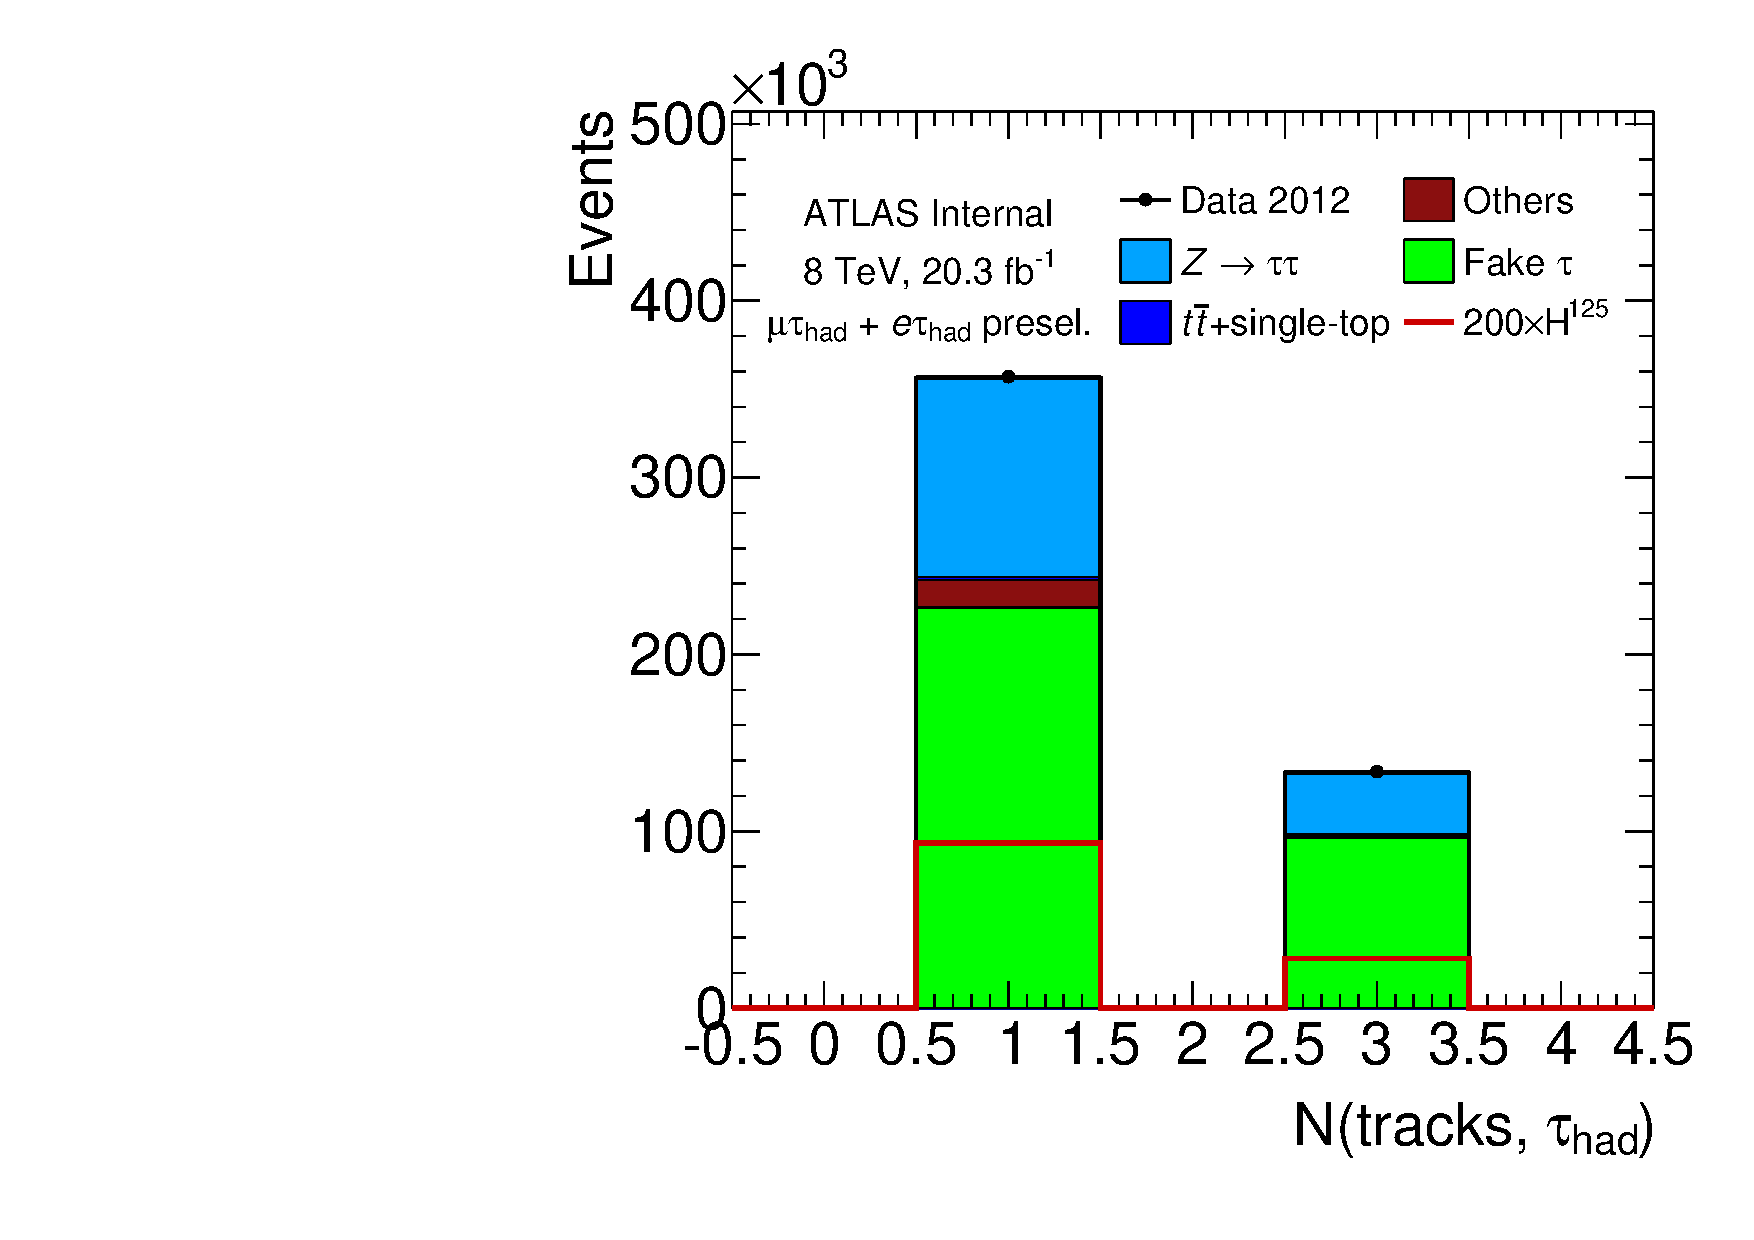
\includegraphics[width=0.32\textwidth]{figures/presel/tau-numTrack} \\
  % --------------
  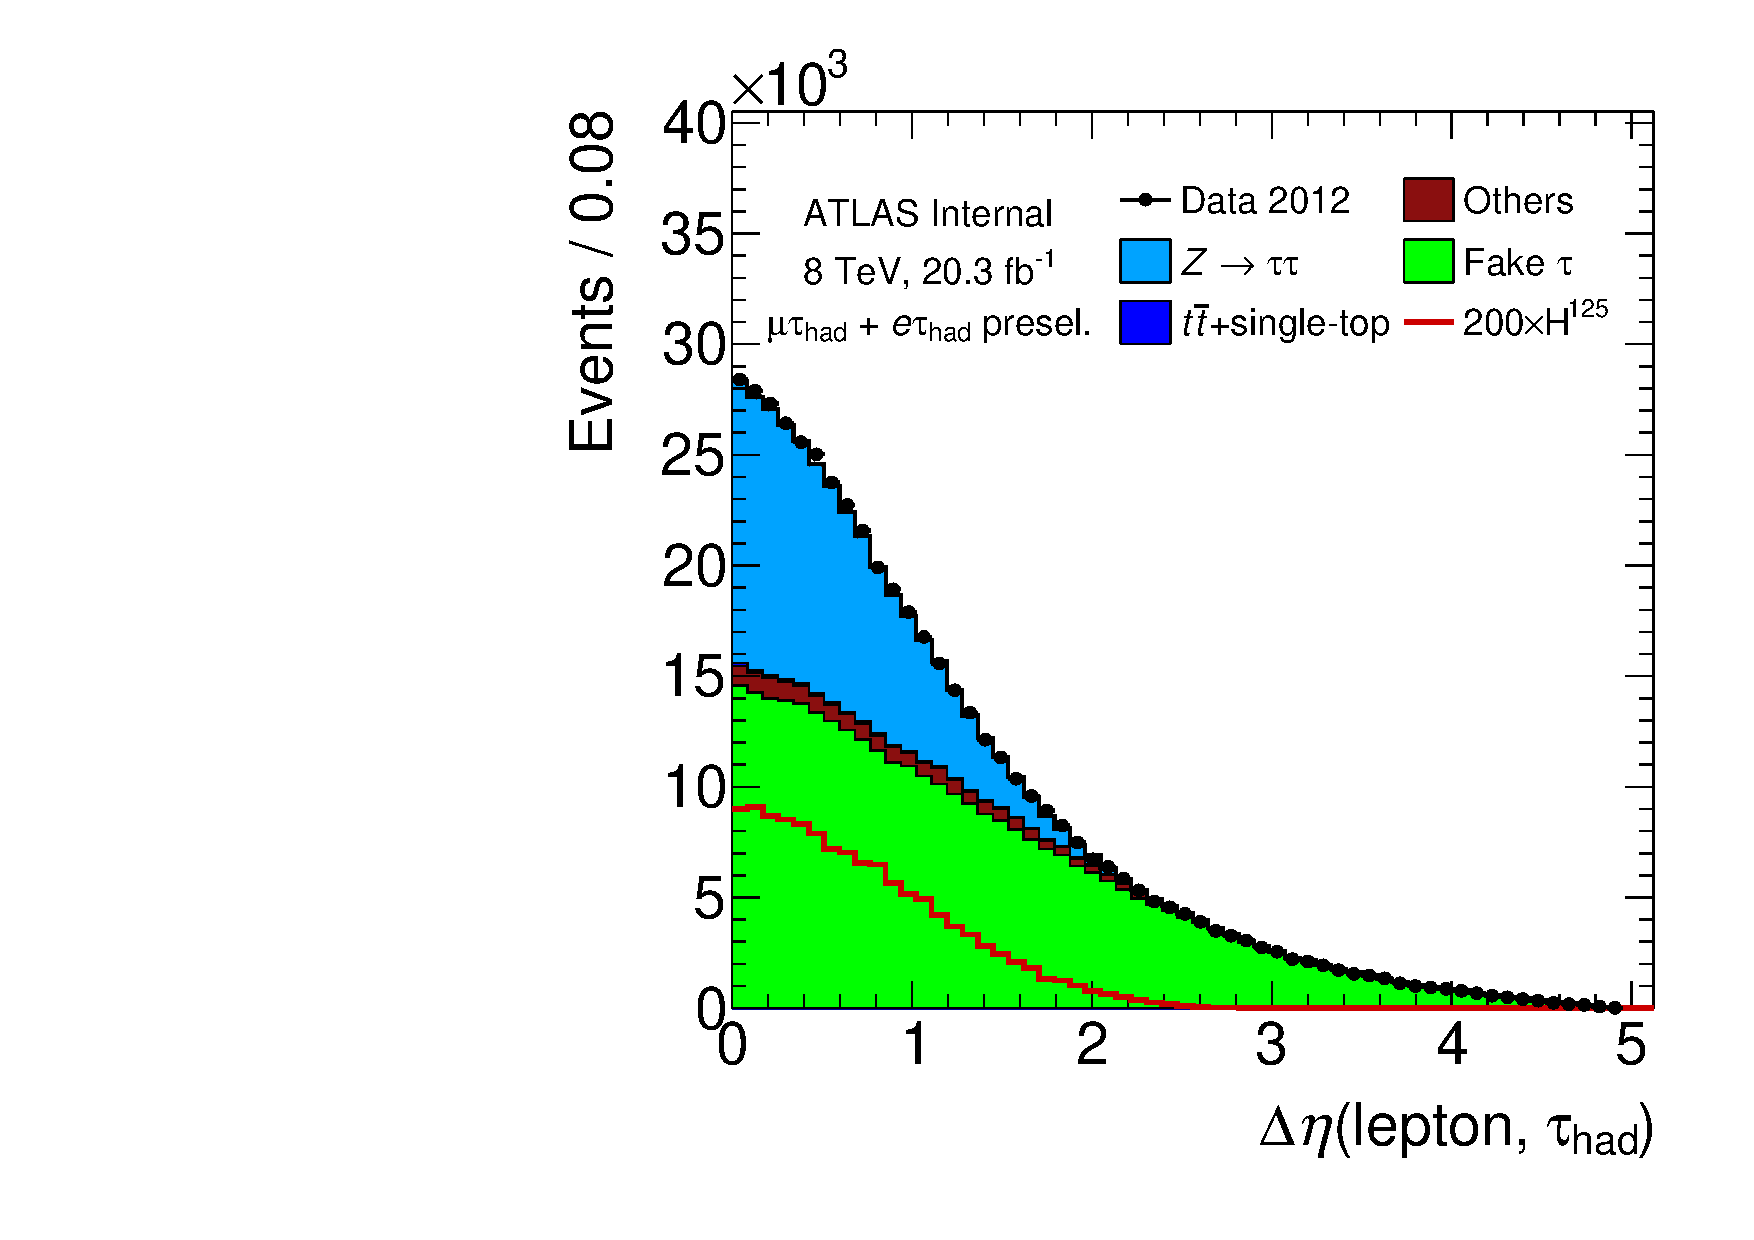
\includegraphics[width=0.32\textwidth]{figures/presel/taulep-deta}
  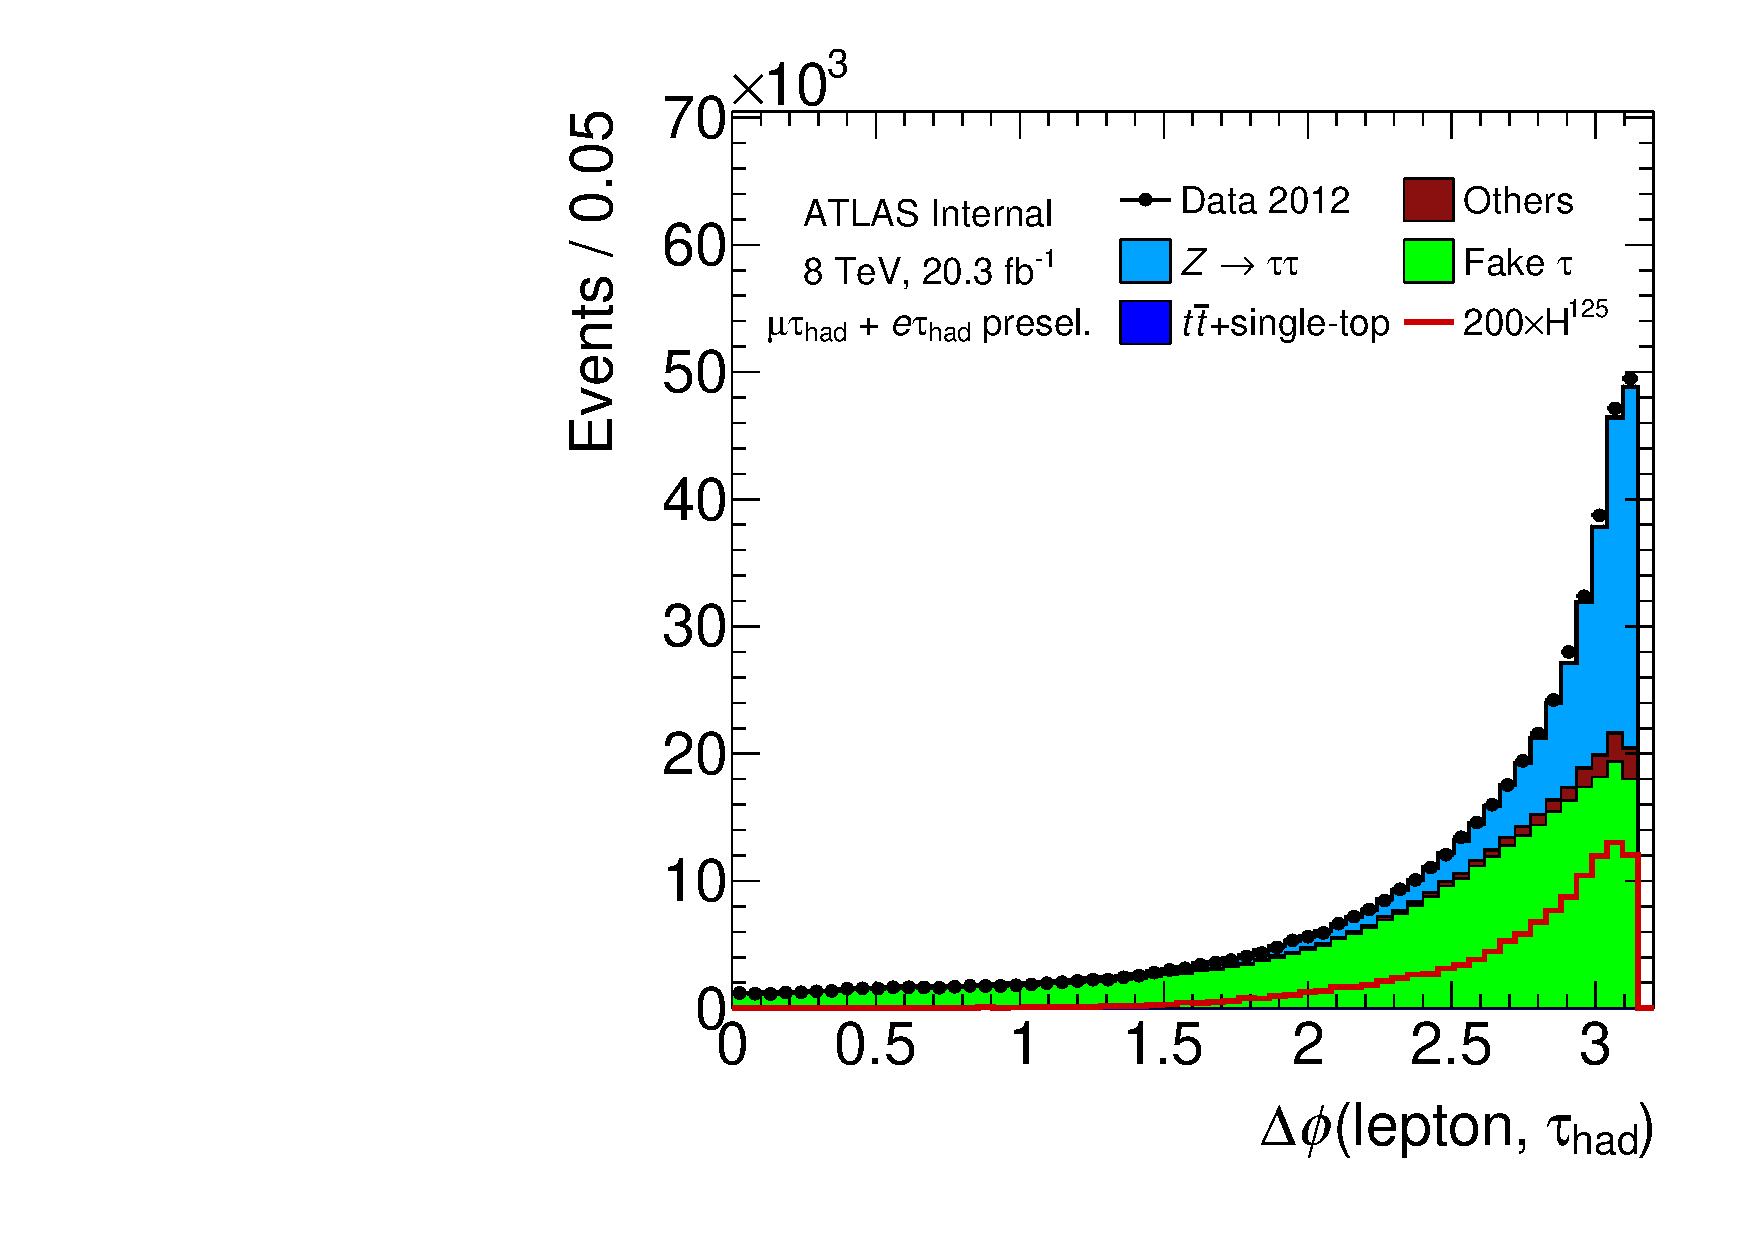
\includegraphics[width=0.32\textwidth]{figures/presel/taulep-dphi}
  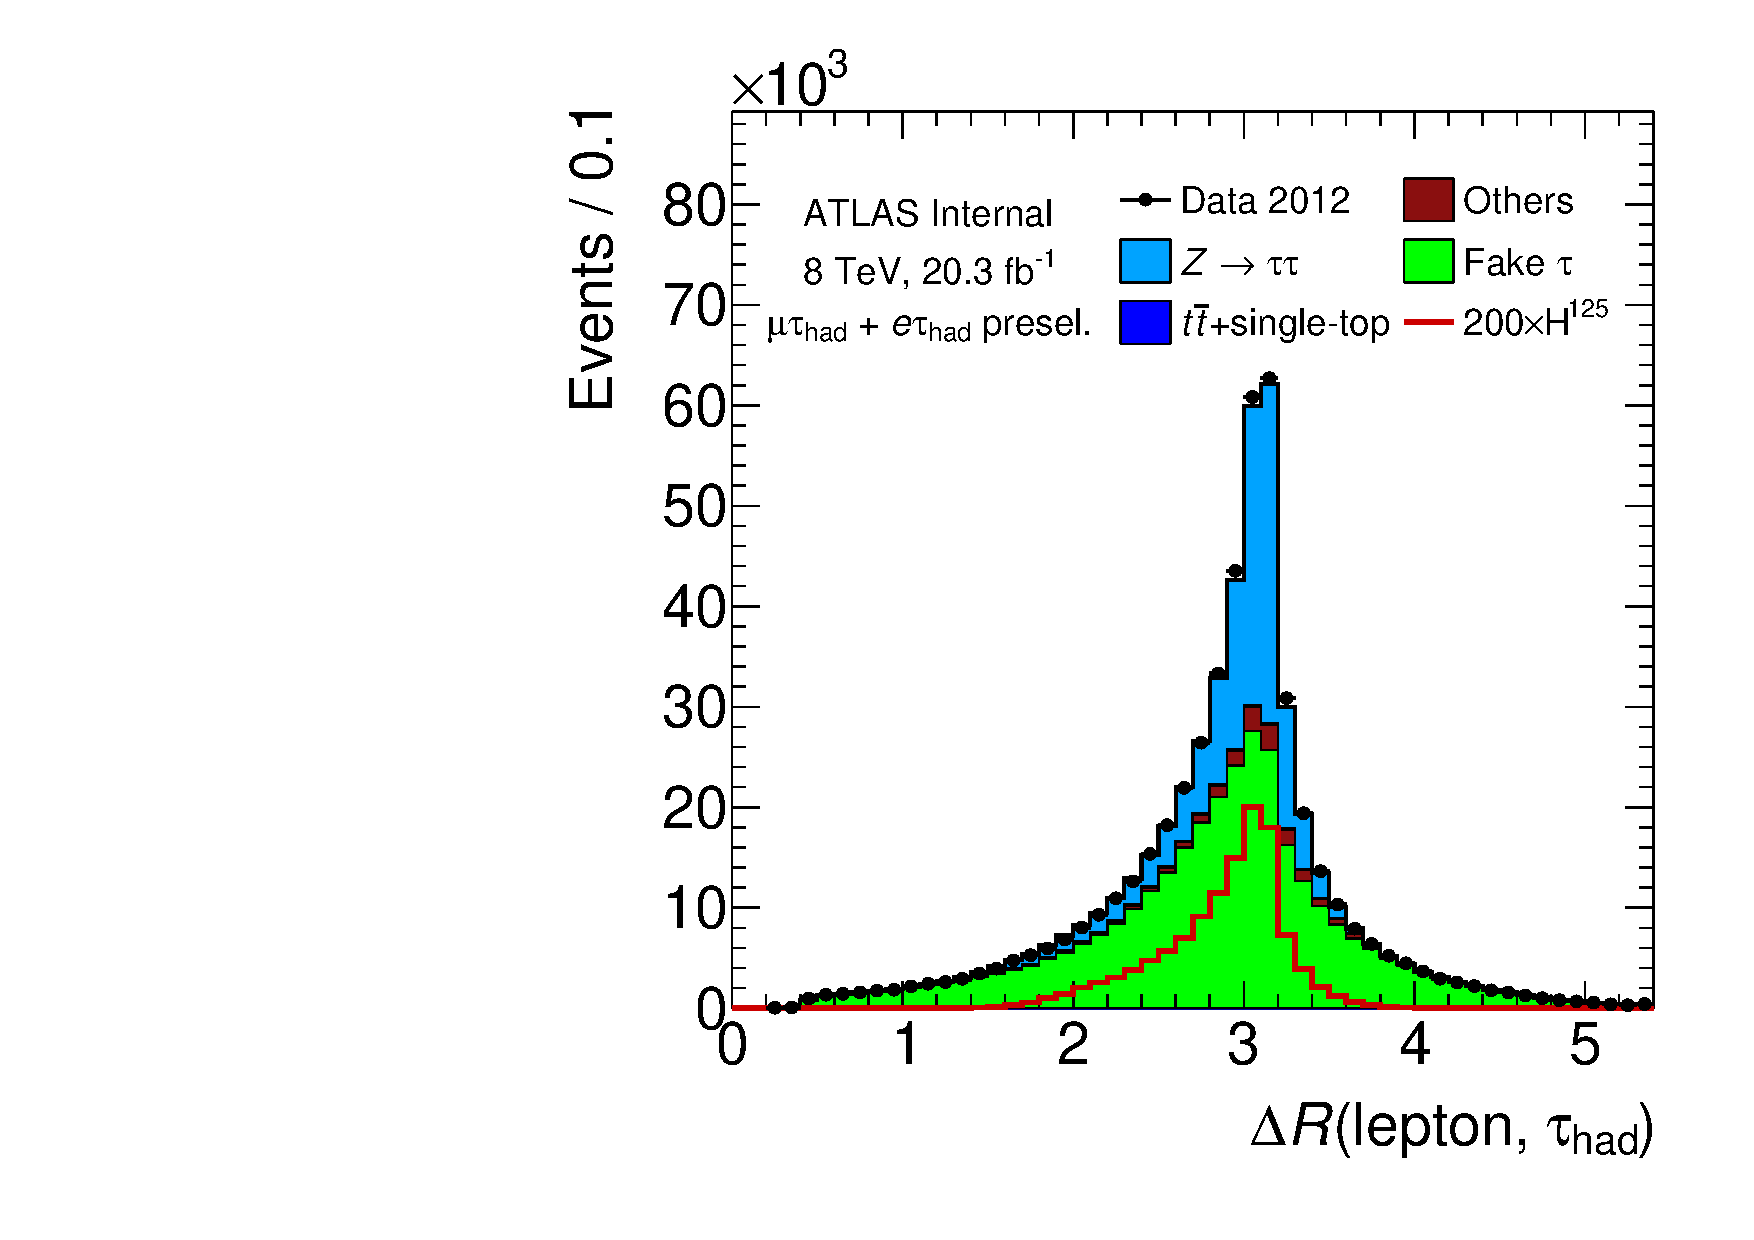
\includegraphics[width=0.32\textwidth]{figures/presel/taulep-dR} \\
  \caption{Kinematic distributions in the pre-selection category of the 8 TeV $\Htautaulh$ analysis with the requirement on $\mT$ removed.}
  \label{fig:stategy-presel-1}
\end{figure}

\clearpage

\begin{figure}[tp]
  \centering
  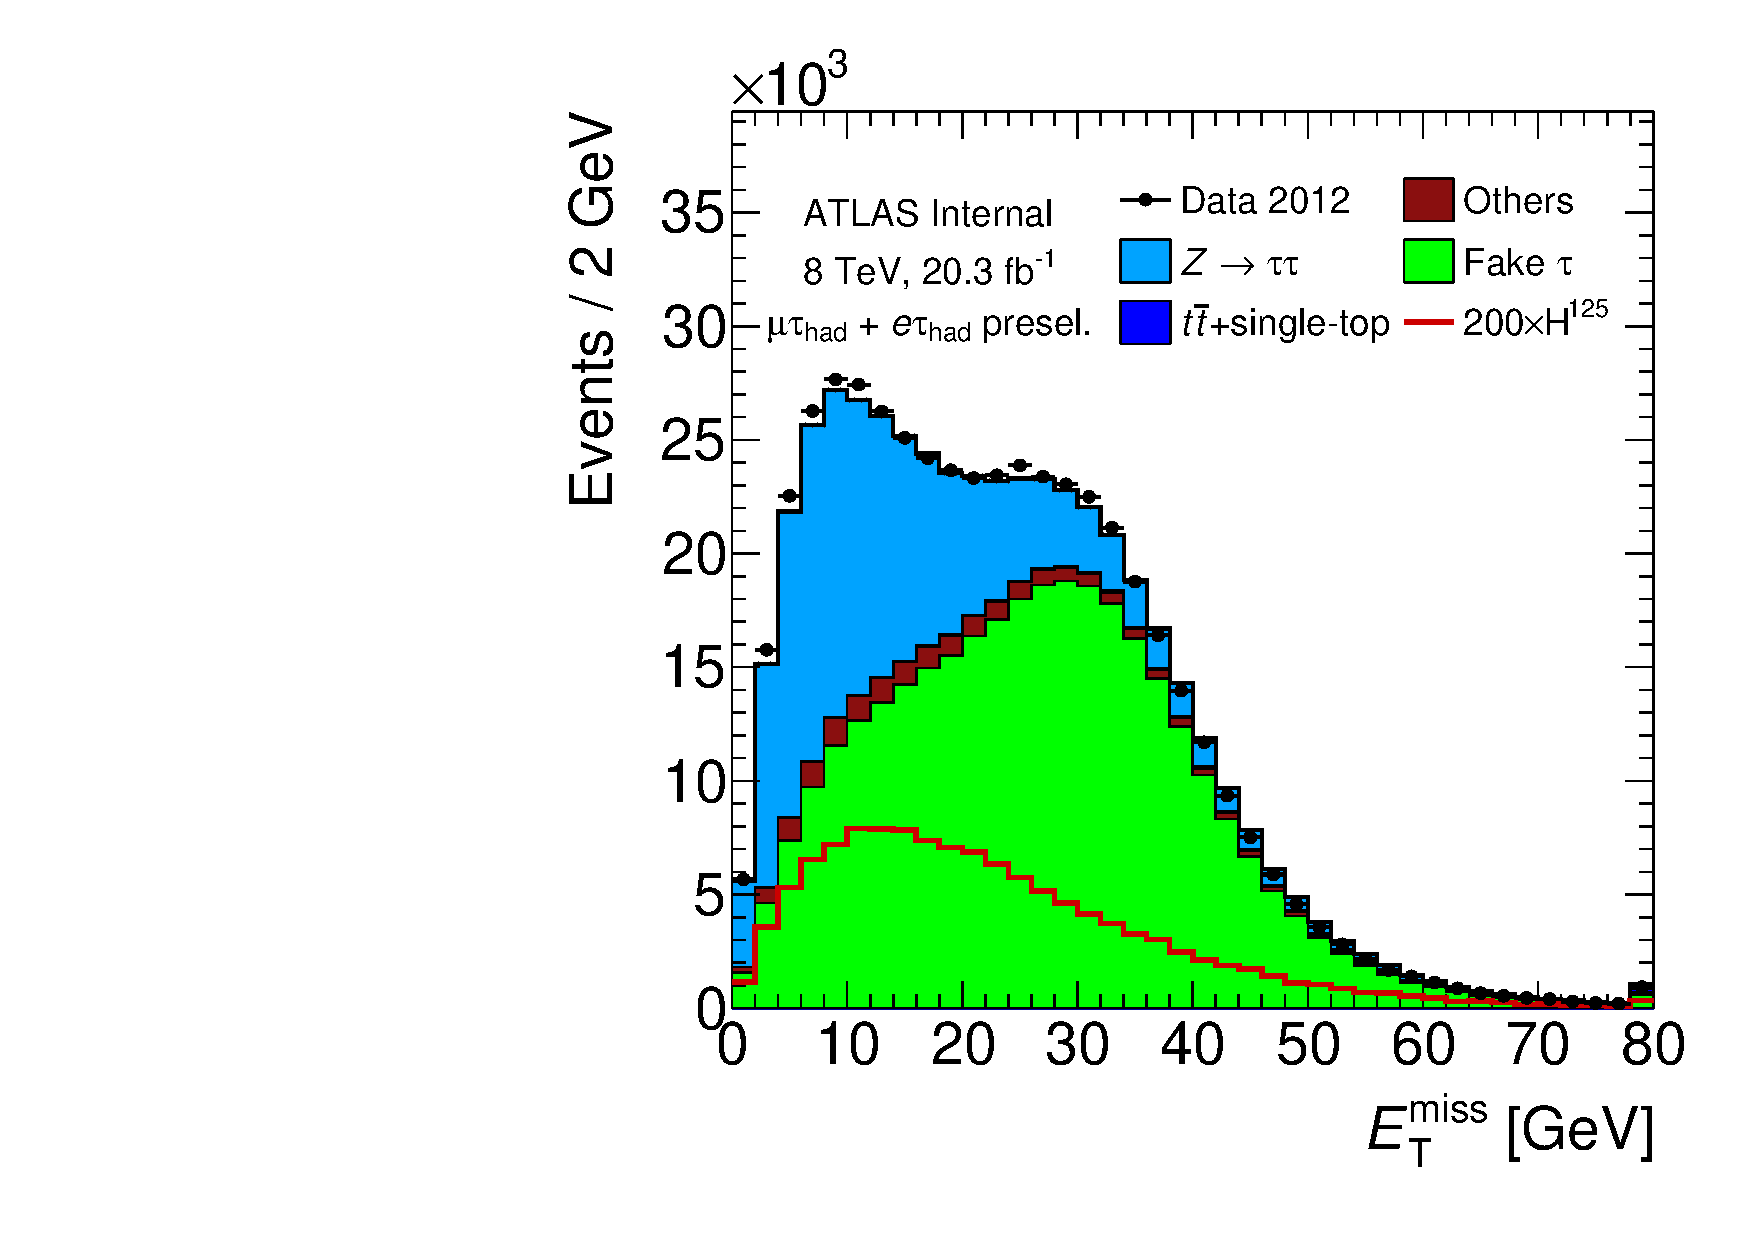
\includegraphics[width=0.32\textwidth]{figures/presel/met-pt}
  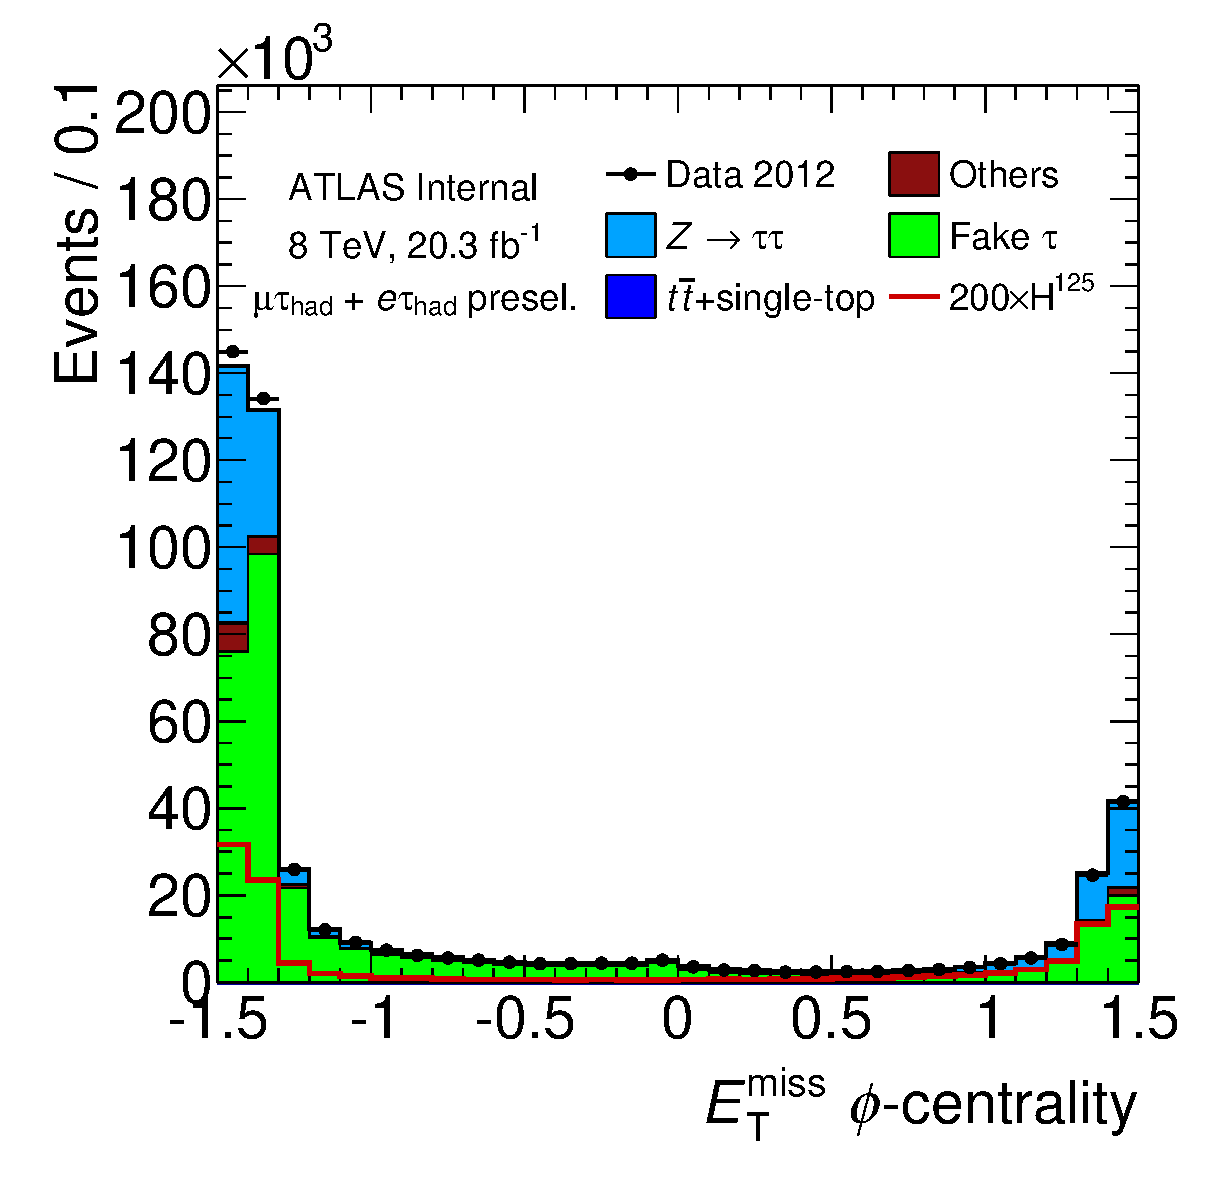
\includegraphics[width=0.32\textwidth]{figures/presel/met-phi-centrality}
  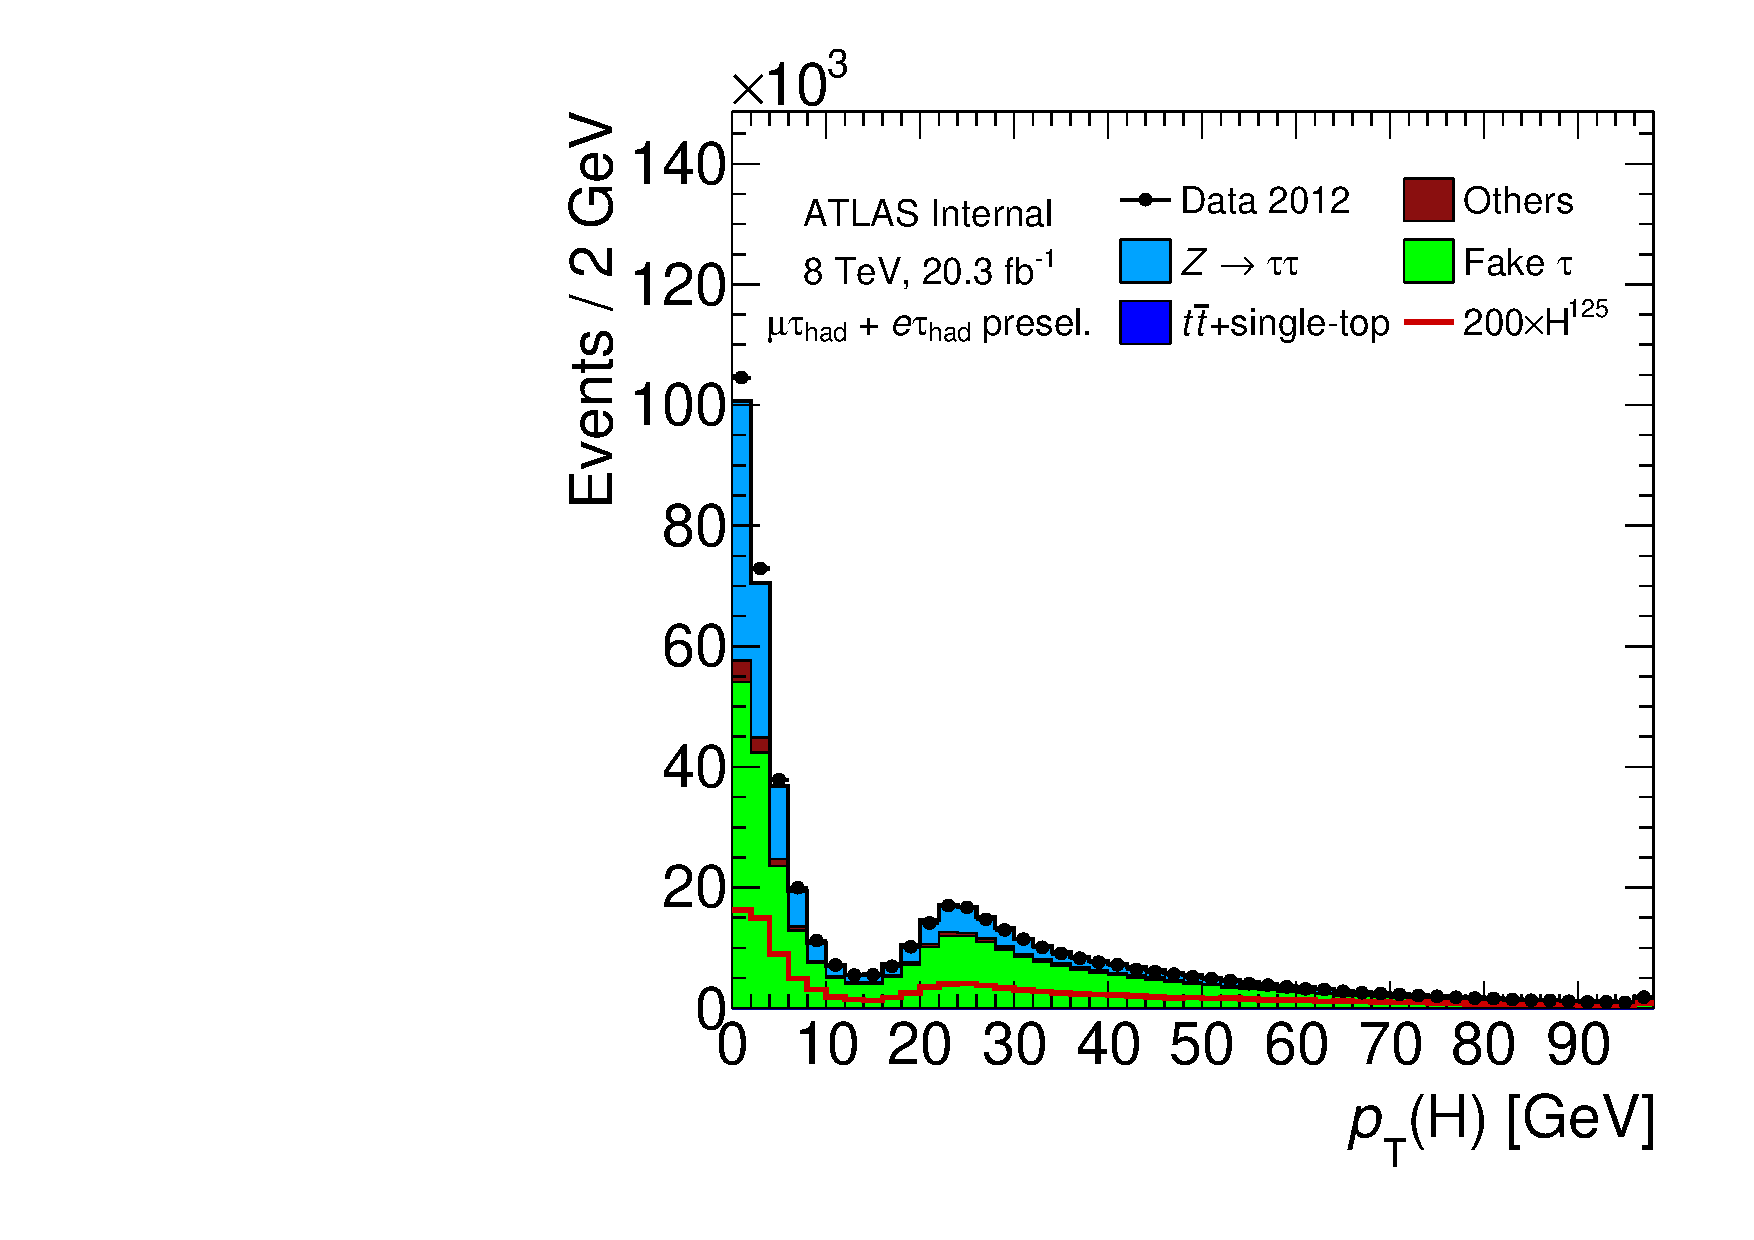
\includegraphics[width=0.32\textwidth]{figures/presel/H-pt} \\
  % --------------
  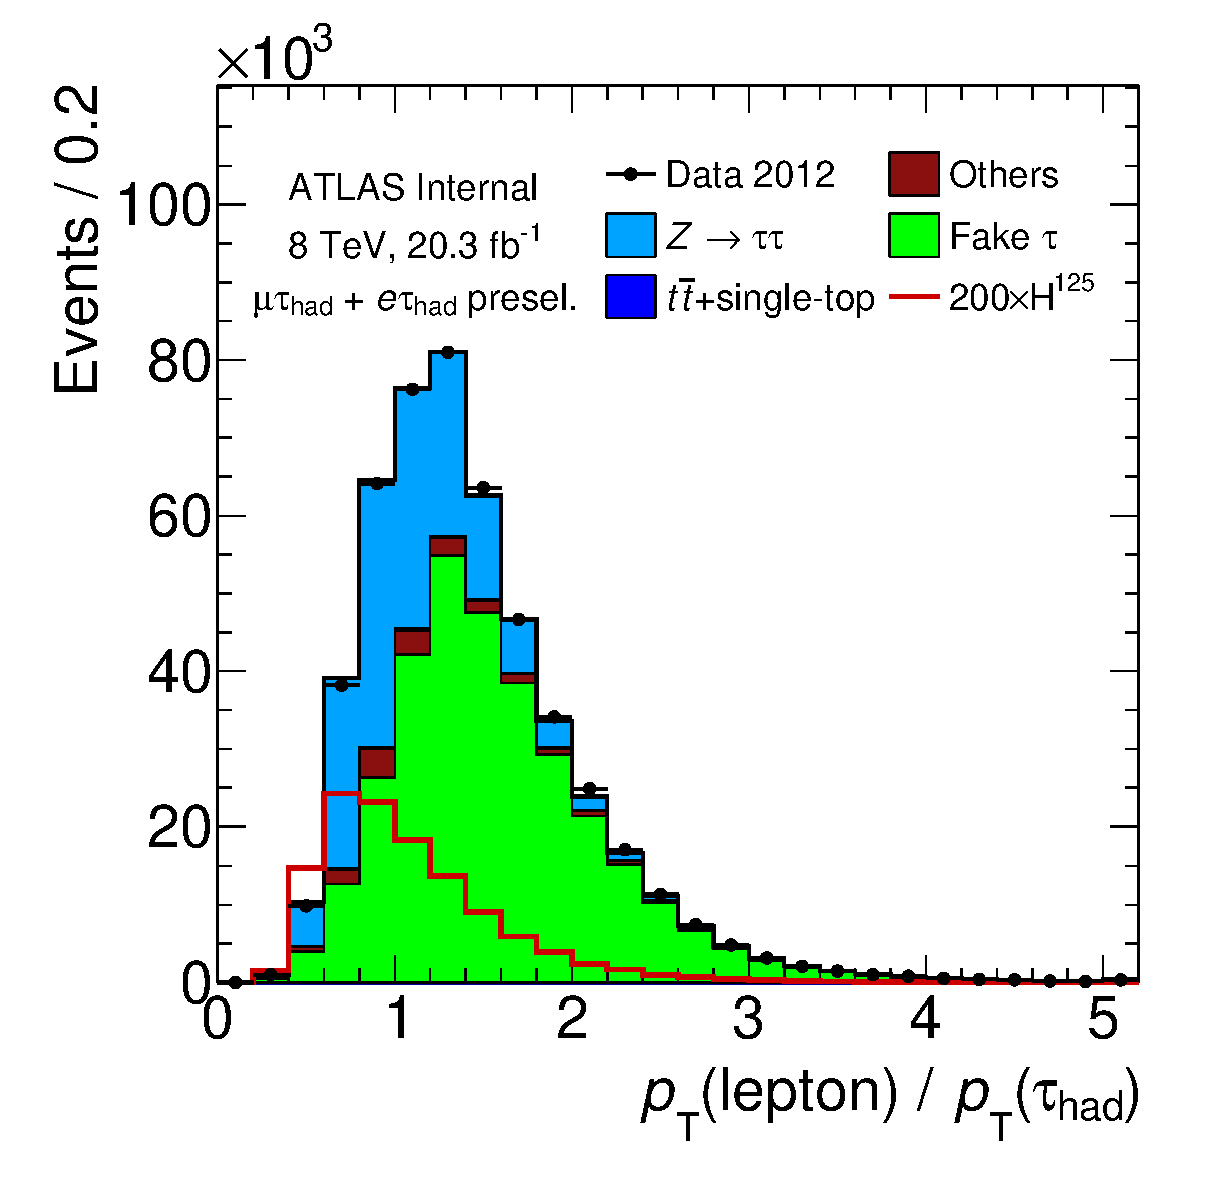
\includegraphics[width=0.32\textwidth]{figures/presel/taulep-ptratio}
  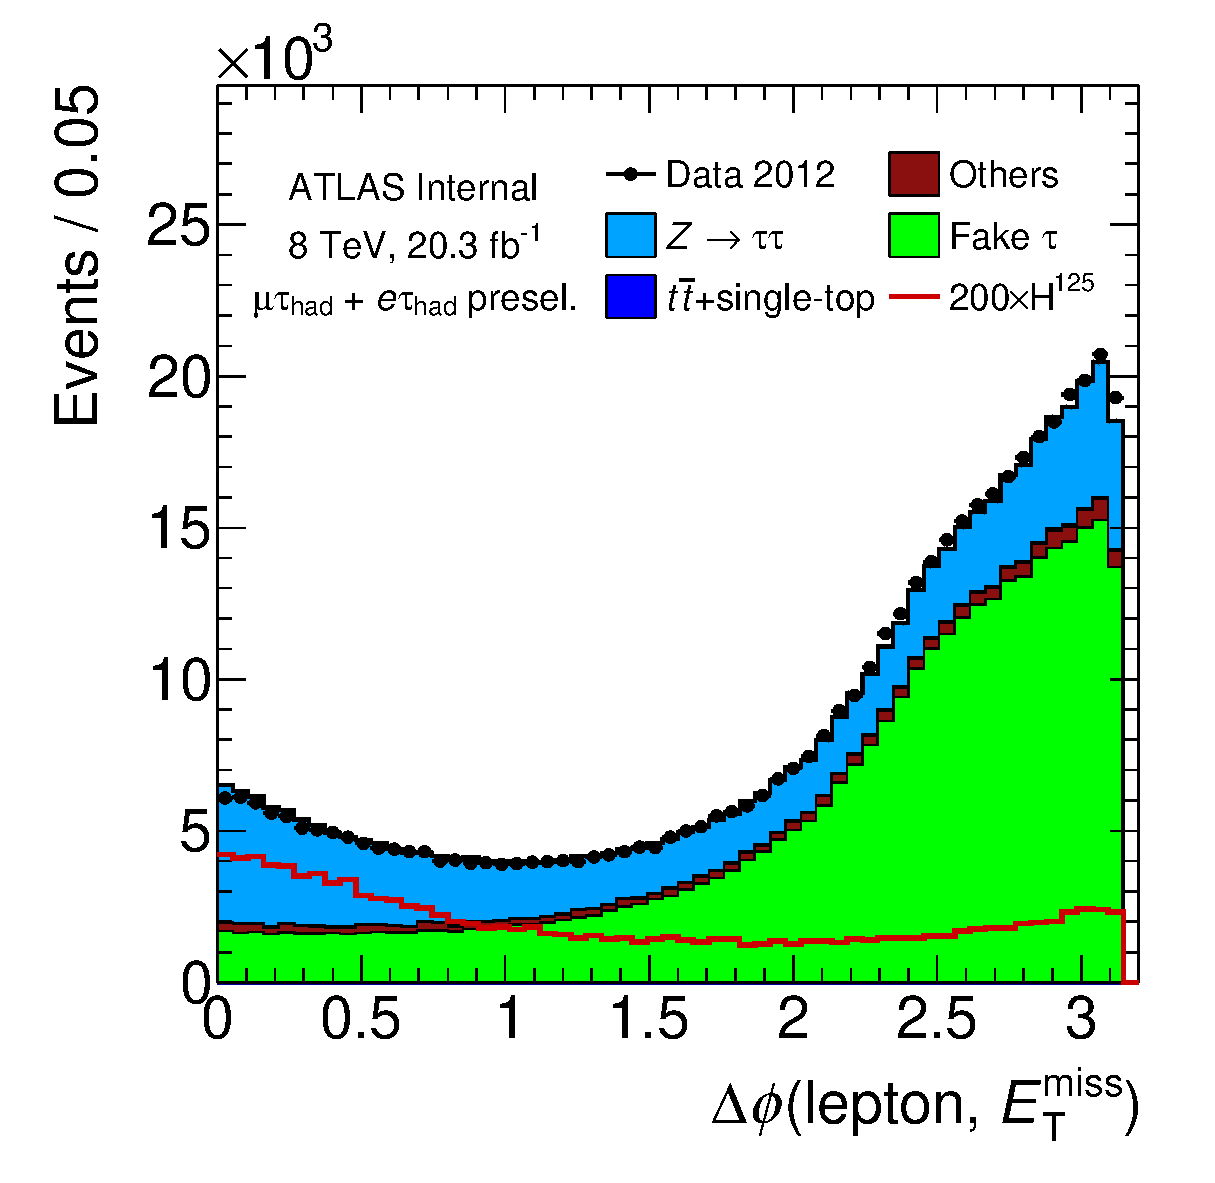
\includegraphics[width=0.32\textwidth]{figures/presel/lepmet-dphi}
  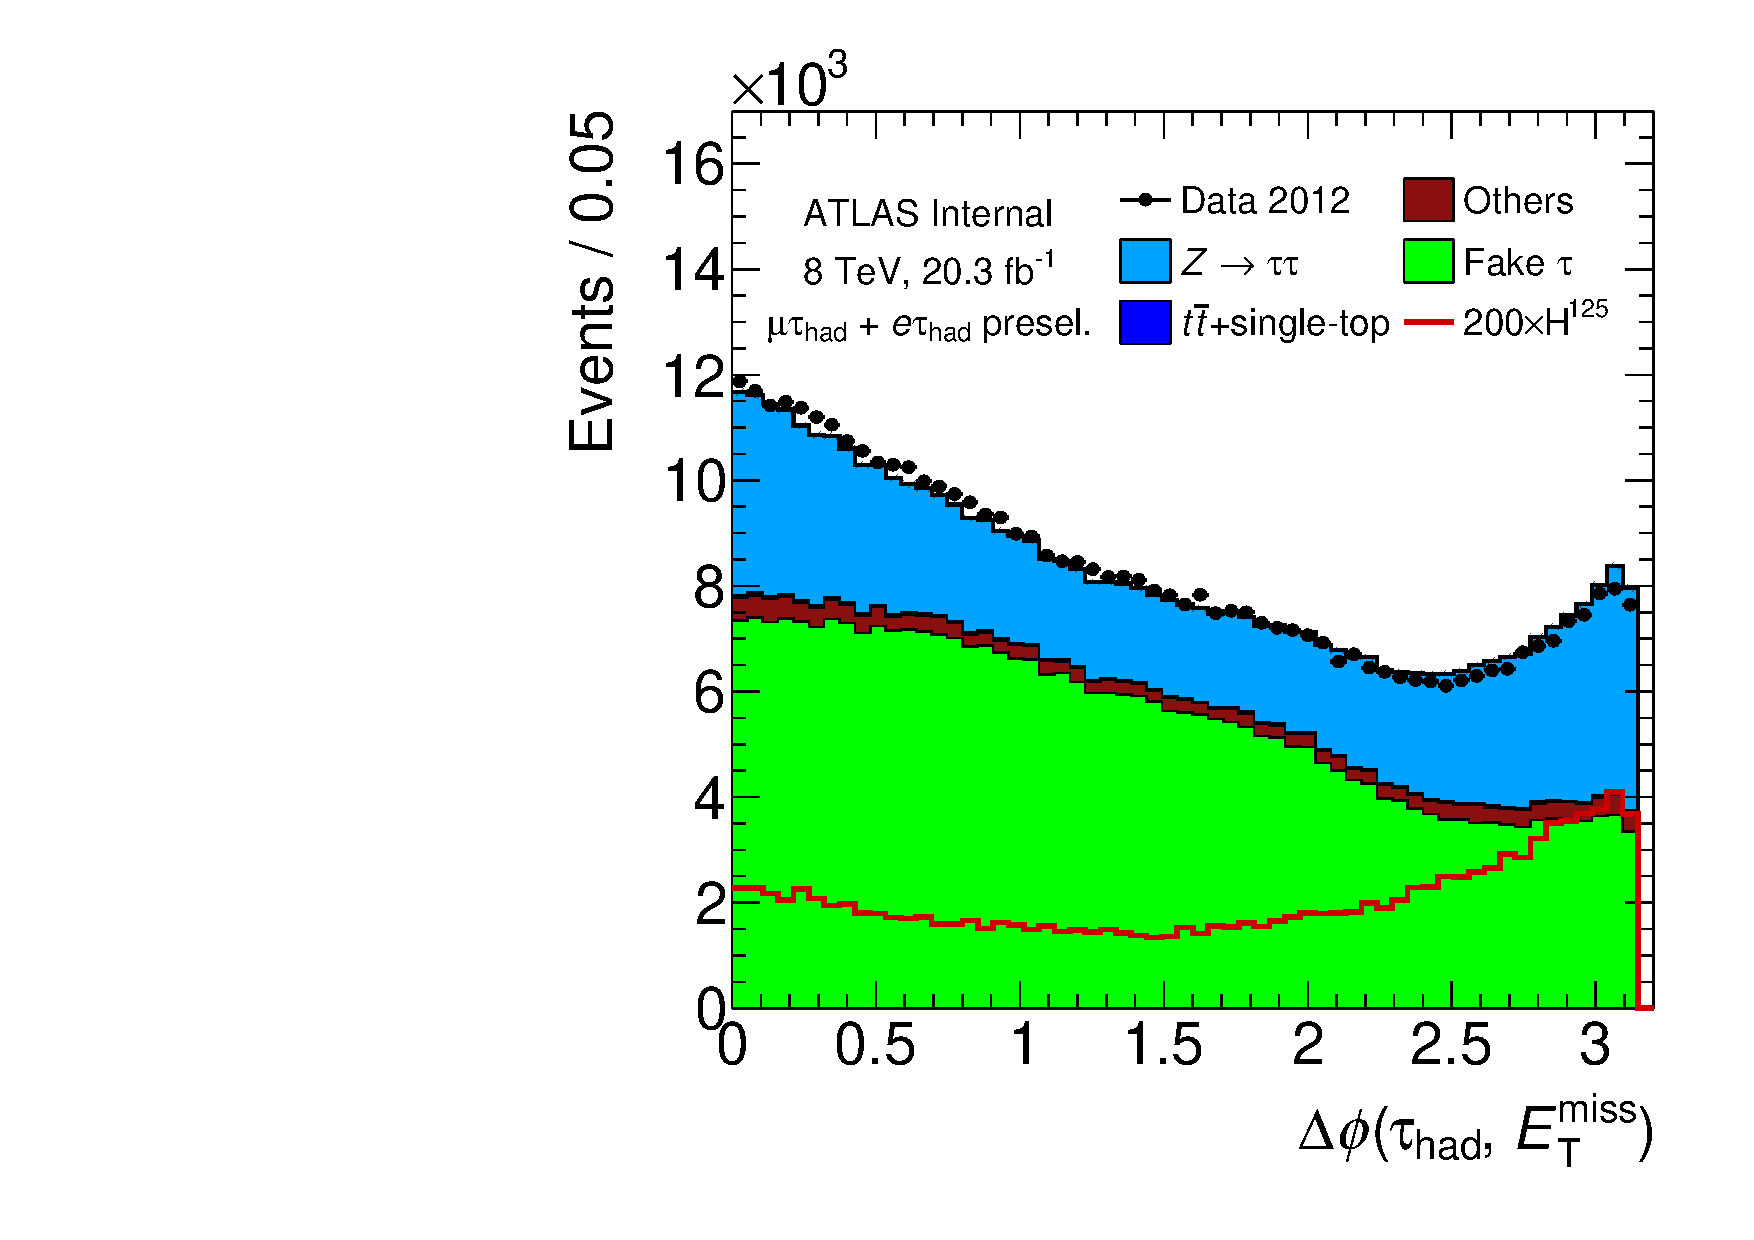
\includegraphics[width=0.32\textwidth]{figures/presel/taumet-dphi} \\
  % --------------
  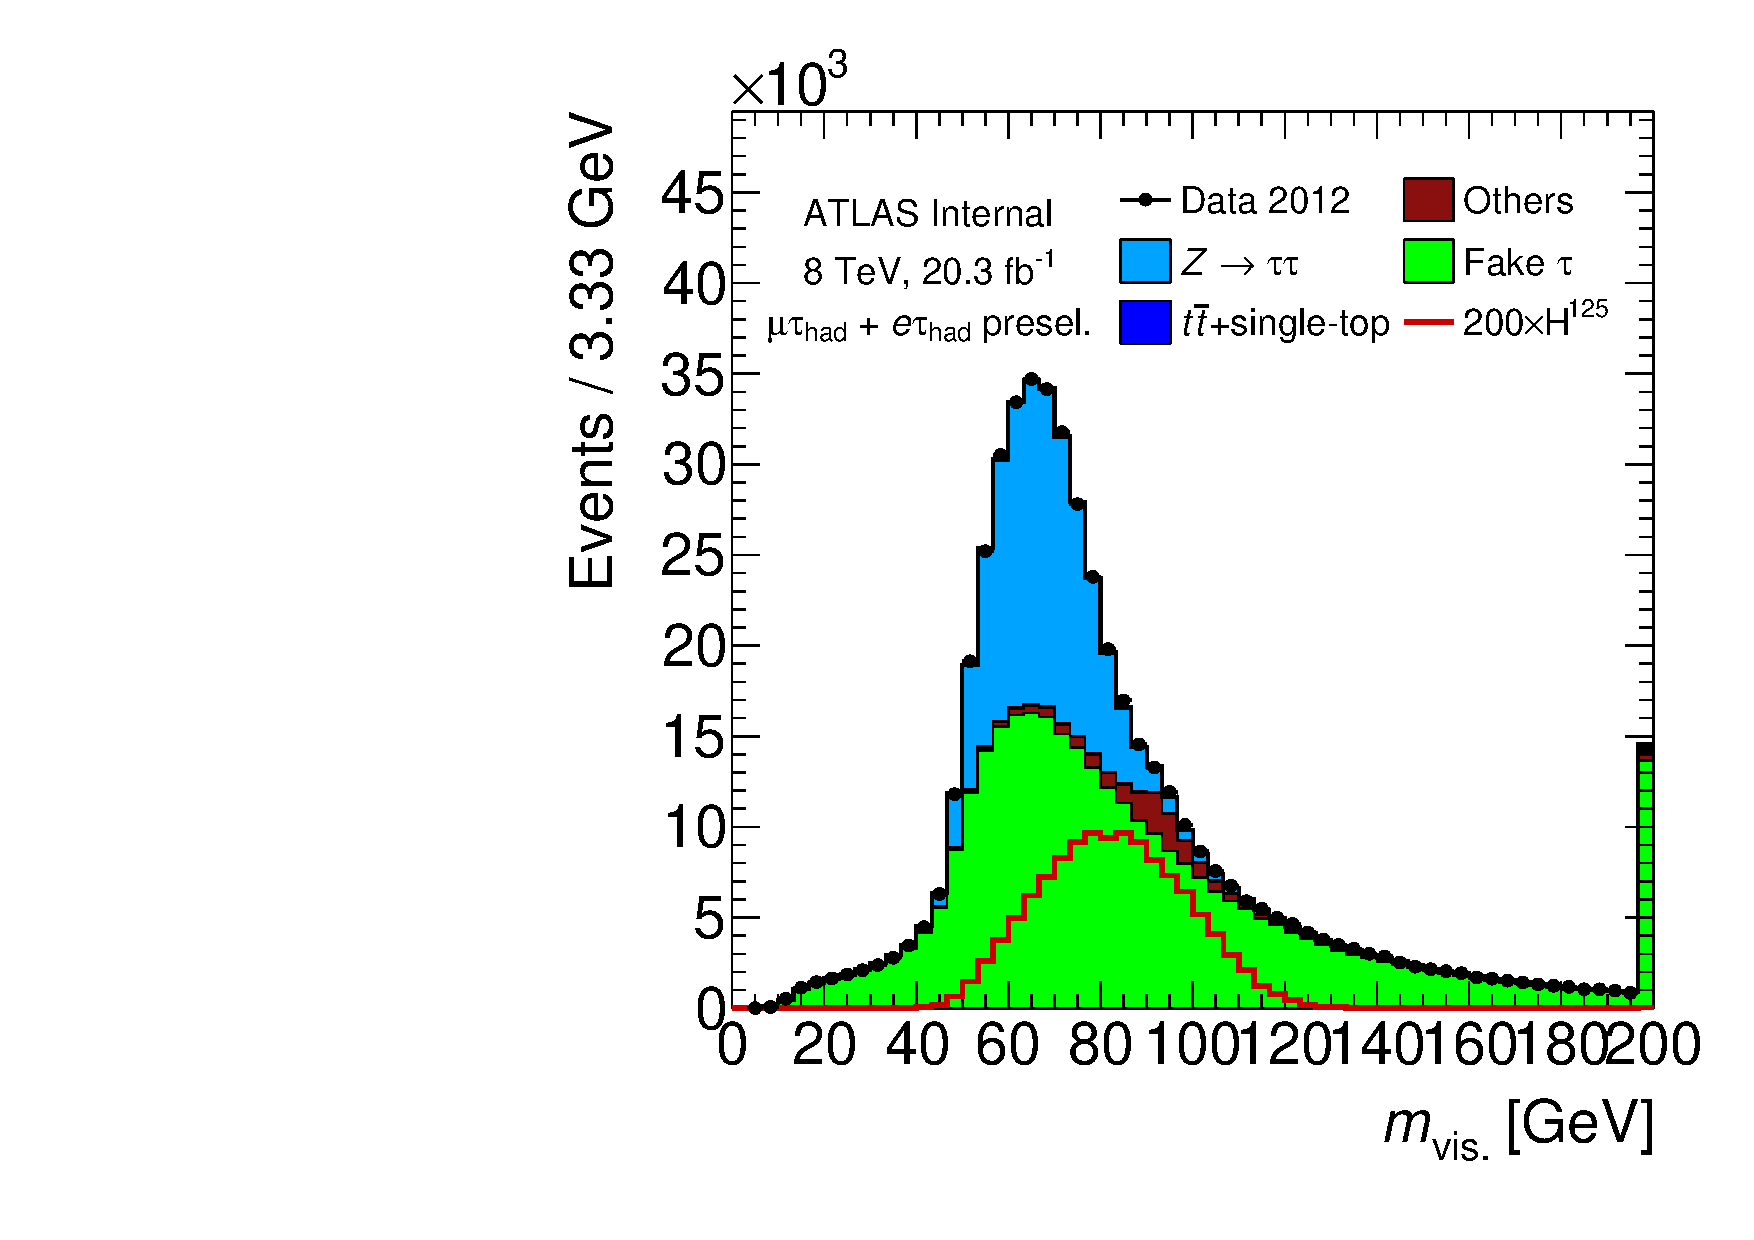
\includegraphics[width=0.32\textwidth]{figures/presel/mvis}
  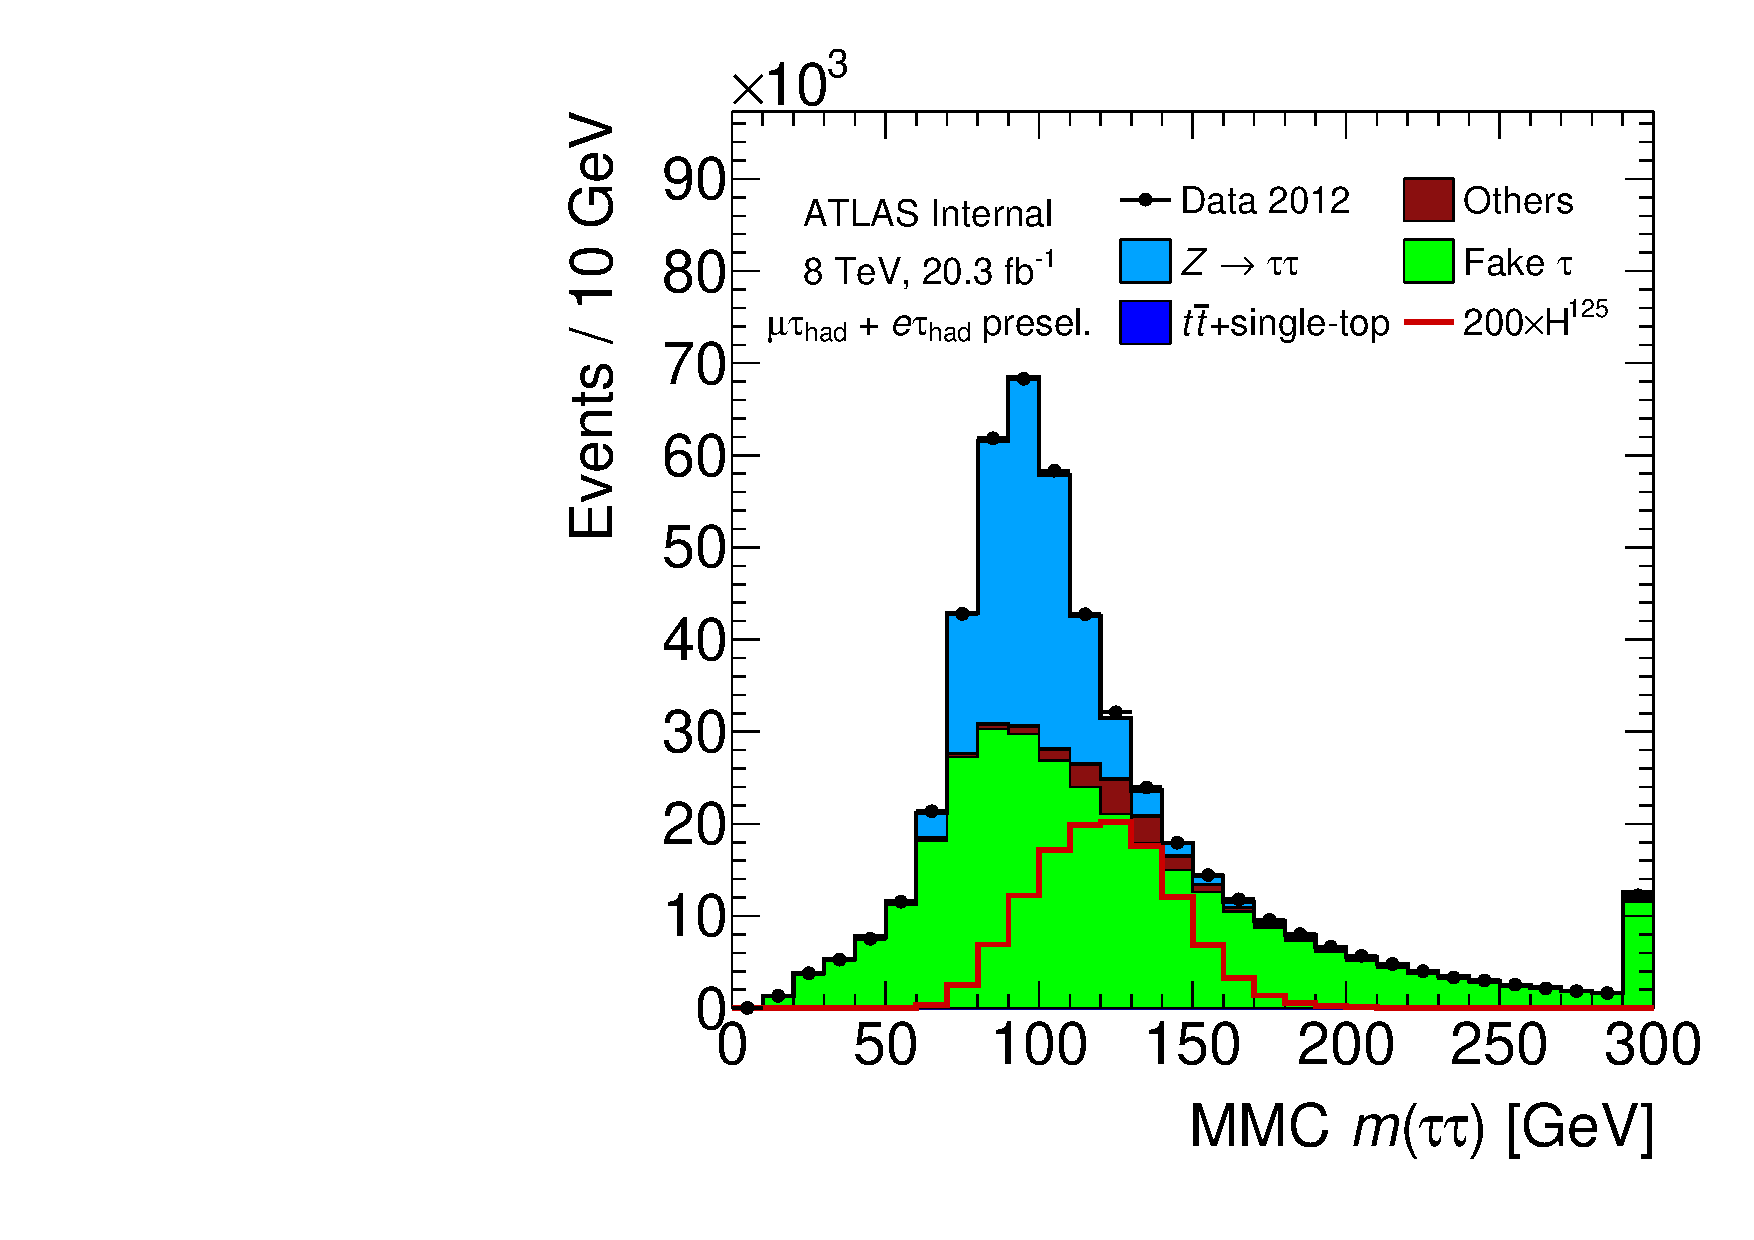
\includegraphics[width=0.32\textwidth]{figures/presel/mMMC}
  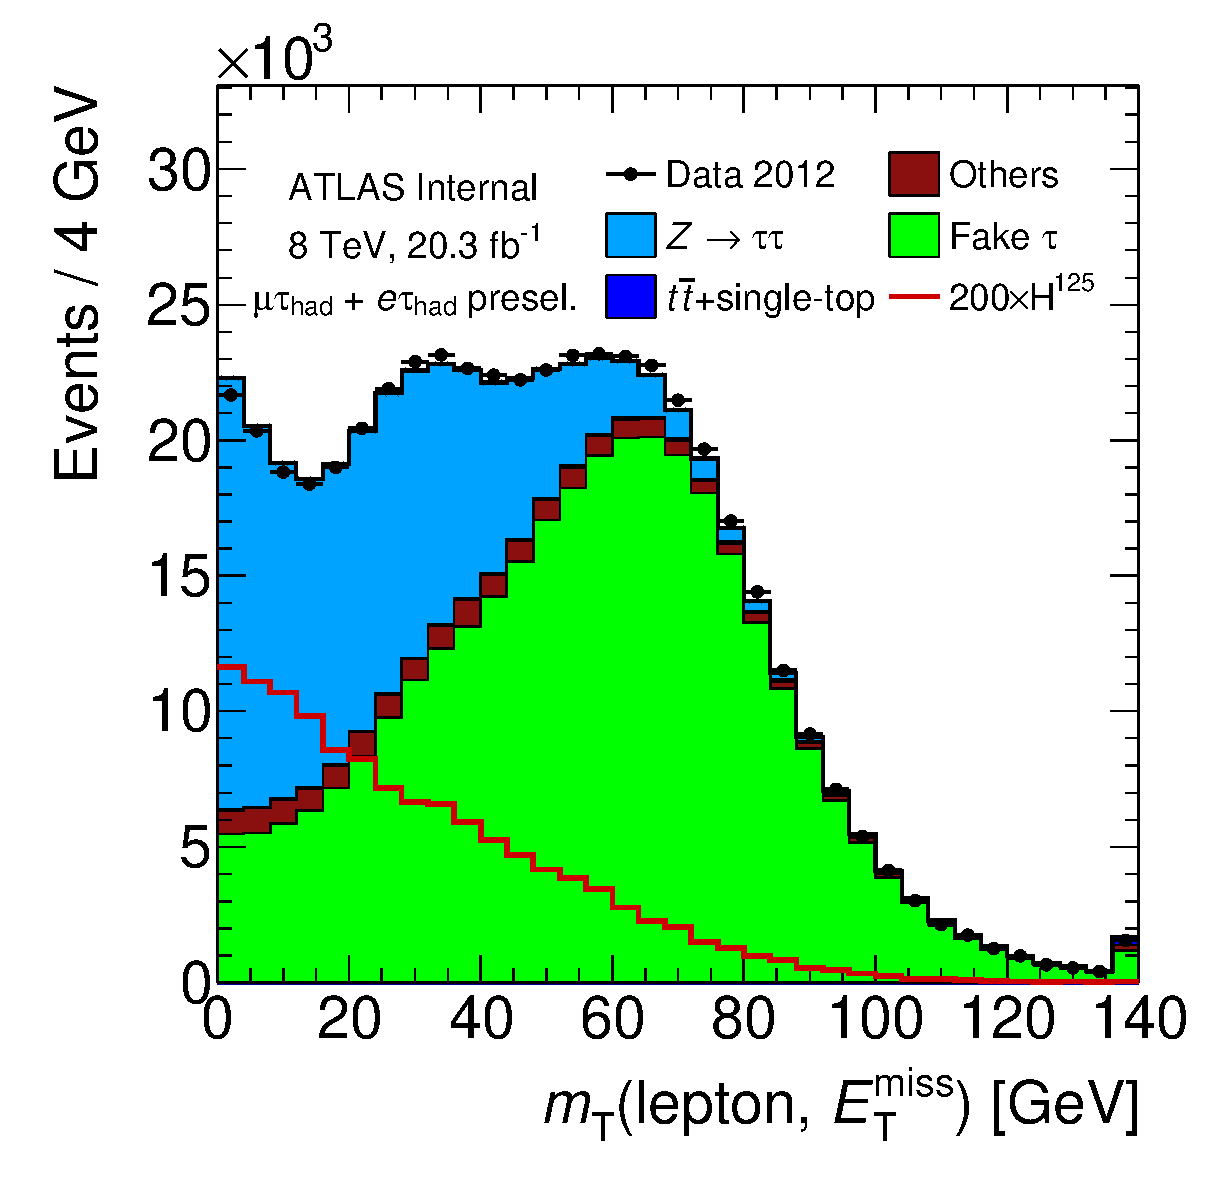
\includegraphics[width=0.32\textwidth]{figures/presel/mT-hi} \\
  % --------------
  \caption{Kinematic distributions in the pre-selection category of the 8 TeV $\Htautaulh$ analysis with the requirement on $\mT$ removed.}
  \label{fig:stategy-presel-2}
\end{figure}

\subsection{VBF category}
\label{sec:strategy-VBF}

Due to the large background from QCD $\Ztautau$ and $\Wjets$ production, the most sensitive search for $\Htautau$ is via the VBF production mechanism~\cite{1998.vbfhtautau}. The signature of this production mechanism is the existence of two jets with large separation in rapidity, and this signature guides the selection criteria of the VBF category.

In addition to the pre-selection criteria, two additional jets are required for the VBF category which satisfy $\Delta\eta(jj) > 3$. The leading and sub-leading jets are assumed to be the VBF jets, and they are required to satisfy the criteria described in \cref{tab:strategy-objects-jetmet}. The threshold on the lead jet is raised to 50 GeV. The visible mass $\mvis$ is also required to be above 40 GeV because discrepancies are observed between data and prediction at very low mass. The VBF category selection is summarized in \cref{tab:strategy-selection}, and similar selection criteria are used to define the VBF $\Htautauhh$ and $\Htautaull$ categories.

\subsection{Boosted category}
\label{sec:strategy-boost}

The second category considered is the boosted category. This category selects events by the transverse boost of the Higgs candidate, where the Higgs candidate is defined as the vector sum of the lepton, $\tauh$, and $\MET$. It is required to have a boost greater than 100 GeV, and similar selection criteria are used to define the boosted $\Htautauhh$ and $\Htautaull$ categories.

This selection emphasizes the ggF Higgs production mechanism with a high $\pt$ ISR jet. The sensitivity of the ggF analysis improves with higher $\pt(H)$ because the $\mtautau$ mass reconstruction techniques have better resolution at smaller $\Delta\phi(\tautau)$. These techniques are discussed in detail in \cref{sec:strategy-mtautau}.

Detailed descriptions of analysis techniques in the boosted category are omitted in this thesis. The focus of the author was on the VBF category, which is more sensitive in searching for $\Htautau$.

\begin{table}[bp]
  \centering
  \renewcommand{\arraystretch}{1.4}
  \caption{Pre-selection and categorization criteria in the $\Htautaulh$ analysis.}
  \begin{tabular}{c|c}
  object   & criteria \\
  \hline\hline
  \multirow{3}{*}{Pre-selection}    & exactly one lepton and one $\tauh$ with opposite charge \\
                                    & no $b$-tagged jets \\
                                    & $\mT < 70$ GeV \\
  \hline
  \multirow{4}{*}{VBF category}     & Pre-selection criteria \\
                                    & At least two jets, with $\pt(\text{lead jet}) > 50$ GeV \\
                                    & $\Delta\eta(jj) > 3$ \\
                                    & $\mvis > 40$ GeV \\
  \hline
  \multirow{2}{*}{Boosted category} & Pre-selection criteria \\
                                    & $\pt^H > 100$ GeV \\
\end{tabular}

  \label{tab:strategy-selection}
\end{table}

\clearpage

\section{$\tautau$ mass reconstruction}
\label{sec:strategy-mtautau}

Because there are three neutrinos in the final state of a $\tautaulh$ decay, the Higgs four-momentum cannot be fully reconstructed as in the $\Hyy$ or $\HZZ$ analyses. Many options exist for reconstructing $\mtautau$ from this under-constrained system, as shown in \cref{tab:strategy-mtautau}.
%
\begin{description}
    \item[Visible mass, $\mvis$:] \hfill \\
      Mass of the visible decay products (lepton and $\tauh$). This is the simplest mass reconstruction and is robust against poor $\MET$ resolution. However, it ignores all information about the $\MET$.
    \item[Total transverse mass, $\mttot$:] \hfill \\
      Transverse mass of the lepton, $\tauh$, and $\MET$. This is another simple mass reconstruction, and it incorporates the $\MET$. However, no prior knowledge of tau lepton decays is utilized.
    \item[Collinear mass, $\mcol$:] \hfill \\
      Mass of the $\tautau$ system assuming the neutrinos are exactly collinear with the visible decay products. This is the first attempt at fully reconstructing a $\tautau$ resonance.
    \item[Missing mass calculator, $\mMMC$:] \hfill \\
      Mass of the $\tautau$ system assuming the neutrinos are approximately collinear with the visible decay products. This is discussed in more detail in \cref{sec:strategy-mtautau-mMMC}.
\end{description}
%

\begin{table}[bp]
  \centering
  \renewcommand{\arraystretch}{1.4}
  \caption{$\mtautau$ reconstruction techniques used in ATLAS publications.}
  \begin{tabular}{c||c|c|c|c}
  $\mtautau$  & $\mvis$              & $\mttot$                      & $\mcol$               & $\mMMC$                   \\
  \hline
  process(es) & $\Ztautau$           & $Z^\prime\rightarrow\tau\tau$ & $\HWW$ vs. $\Ztautau$ & $\Htautau$ vs. $\Ztautau$ \\
  publication & \cite{PERF-2013-06}  & \cite{EXOT-2012-03}           & \cite{HIGG-2013-13}   & \cite{HIGG-2013-32}       \\
\end{tabular}

  \label{tab:strategy-mtautau}
\end{table}

\subsection{$\mMMC$ algorithm}
\label{sec:strategy-mtautau-mMMC}

The Missing Mass Calculator $\mMMC$ is used to fully reconstruct $\mtautau$~\cite{2011.mmc}. This requires solving an underconstrained system of equations for seven unknowns in the $\tautaulh$ final state: $x$-, $y$-, and $z$-components of the momentum carried by the neutrinos for each of the tau leptons in the event, and the invariant mass of the $\nu\nu$ system from the leptonic tau decay. The calculation uses the constraints from the measured $x$- and $y$-components of the $\MET$, and the visible masses of both tau lepton decays. A scan is performed over the two components of the $\MET$ vector and the yet undetermined variables. Each scan point is weighted by its probability according to the $\MET$ resolution and the tau decay topologies. The estimator for the $\mtautau$ is defined as the most probable value of the scan points. A cartoon visualization of the technique is shown in \cref{fig:strategy-mtautau-cartoon}.

\begin{figure}[tp]
  \centering
  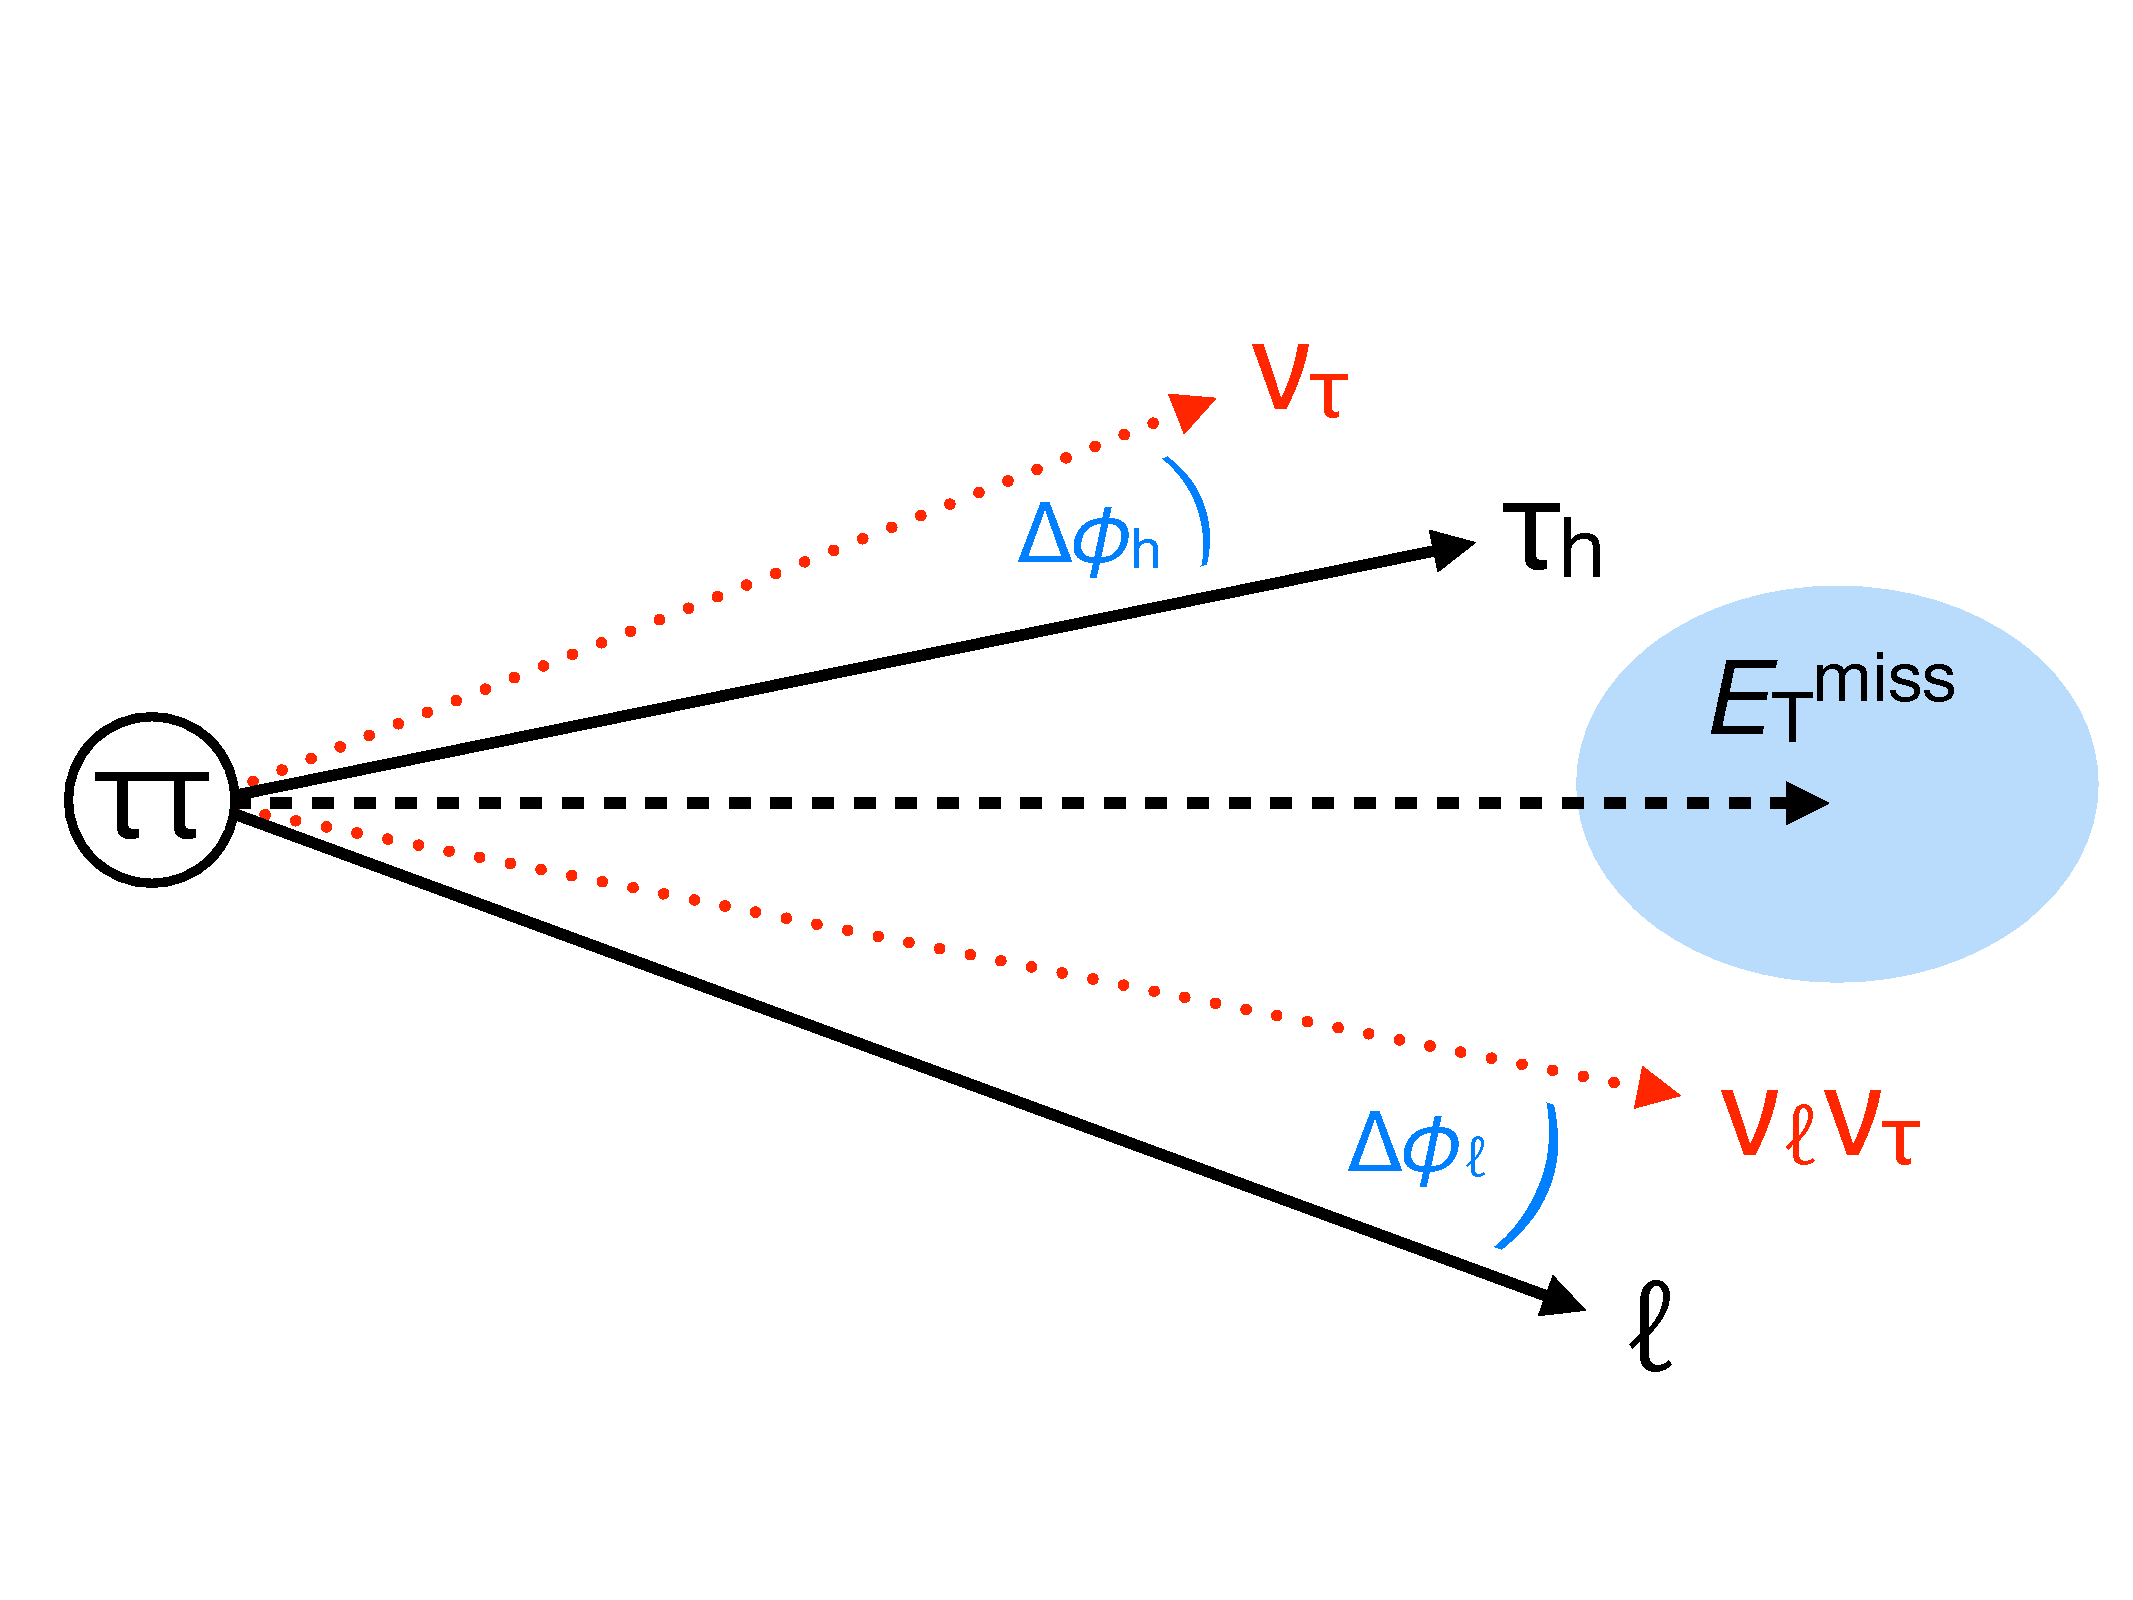
\includegraphics[width=0.90\textwidth]{figures/mtautau/mmc-cartoon}
  \caption{Cartoon of the $\mMMC$ reconstruction algorithm. Black, filled lines indicate items measured directly ($\ell$, $\tauh$). Red, dotted lines indicate items which cannot be measured (neutrinos). The black, dashed line indicates the $\MET$, which is measured indirectly. Blue indicates items which the $\mMMC$ scans to find an optimal solution ($\Delta\phi$, $\MET$).}
  \label{fig:strategy-mtautau-cartoon}
\end{figure}

The multi-dimensional scan requires probability density functions (PDFs) for each dimension, and the final probability is a product of each PDF evaluated at a given scan point. Scans of the $x$- and $y$-components of the $\MET$ use Gaussian PDFs where the mean is the measured $\MEx$ and $\MEy$, respectively, and the standard deviation is the resolution inferred from the measured $\Sigma \text{E}_\text{T}$ of the event. The PDFs of the tau decay topologies are derived from simulated $\Ztautau$ events and shown in \cref{fig:strategy-mtautau-inputs} for a given $\pt$ range.

\begin{figure}[tp]
  \centering
  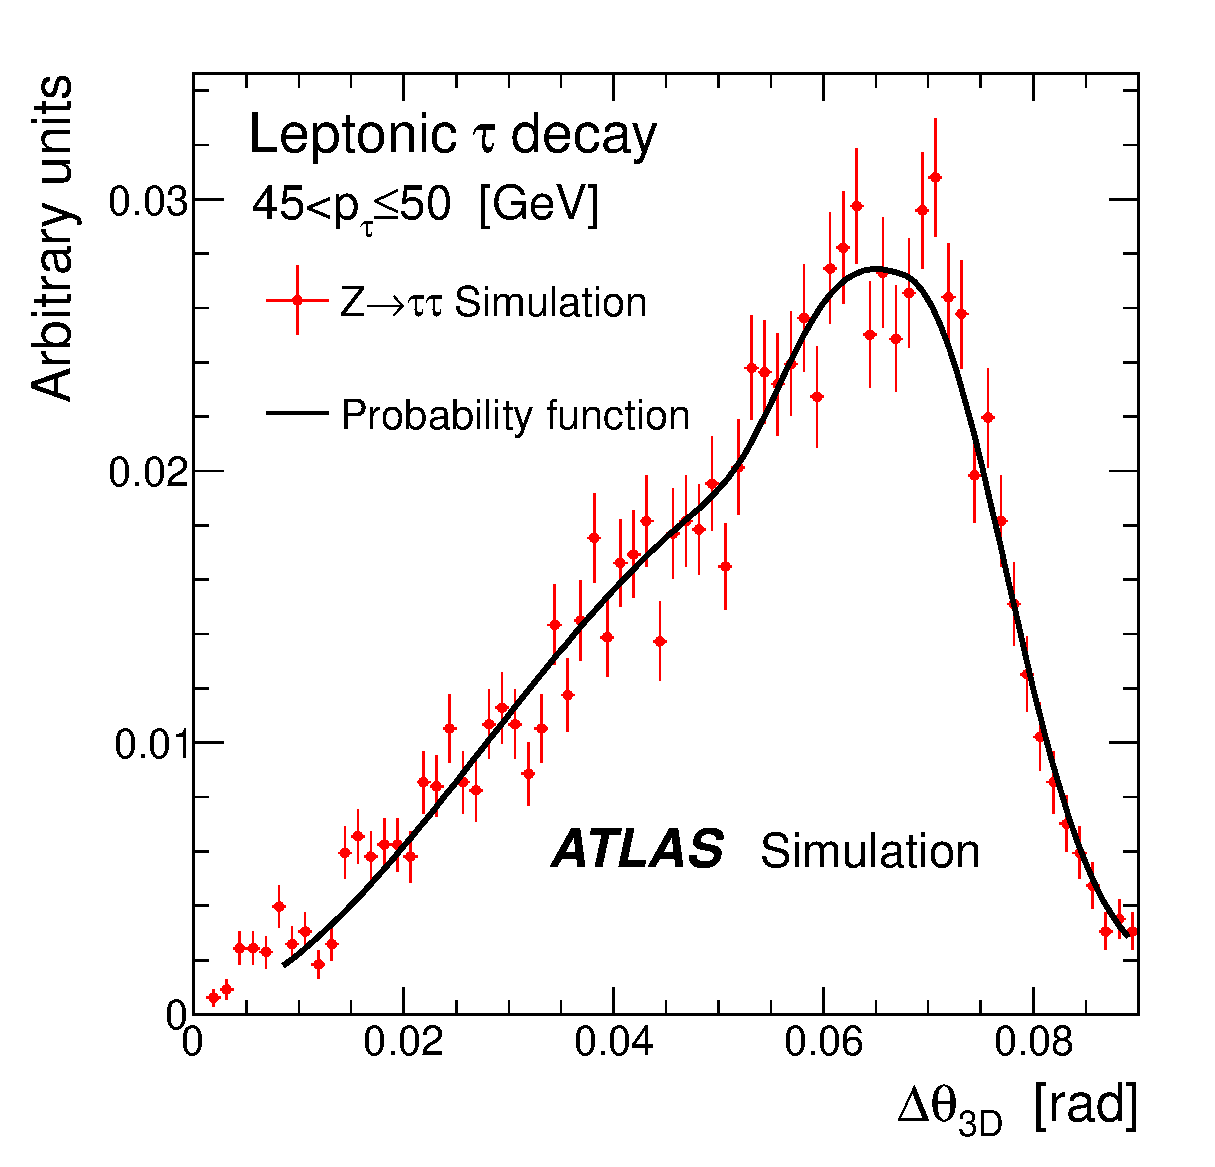
\includegraphics[width=0.32\textwidth]{figures/ATLAS-CONF-2011-132/fig_01a}
  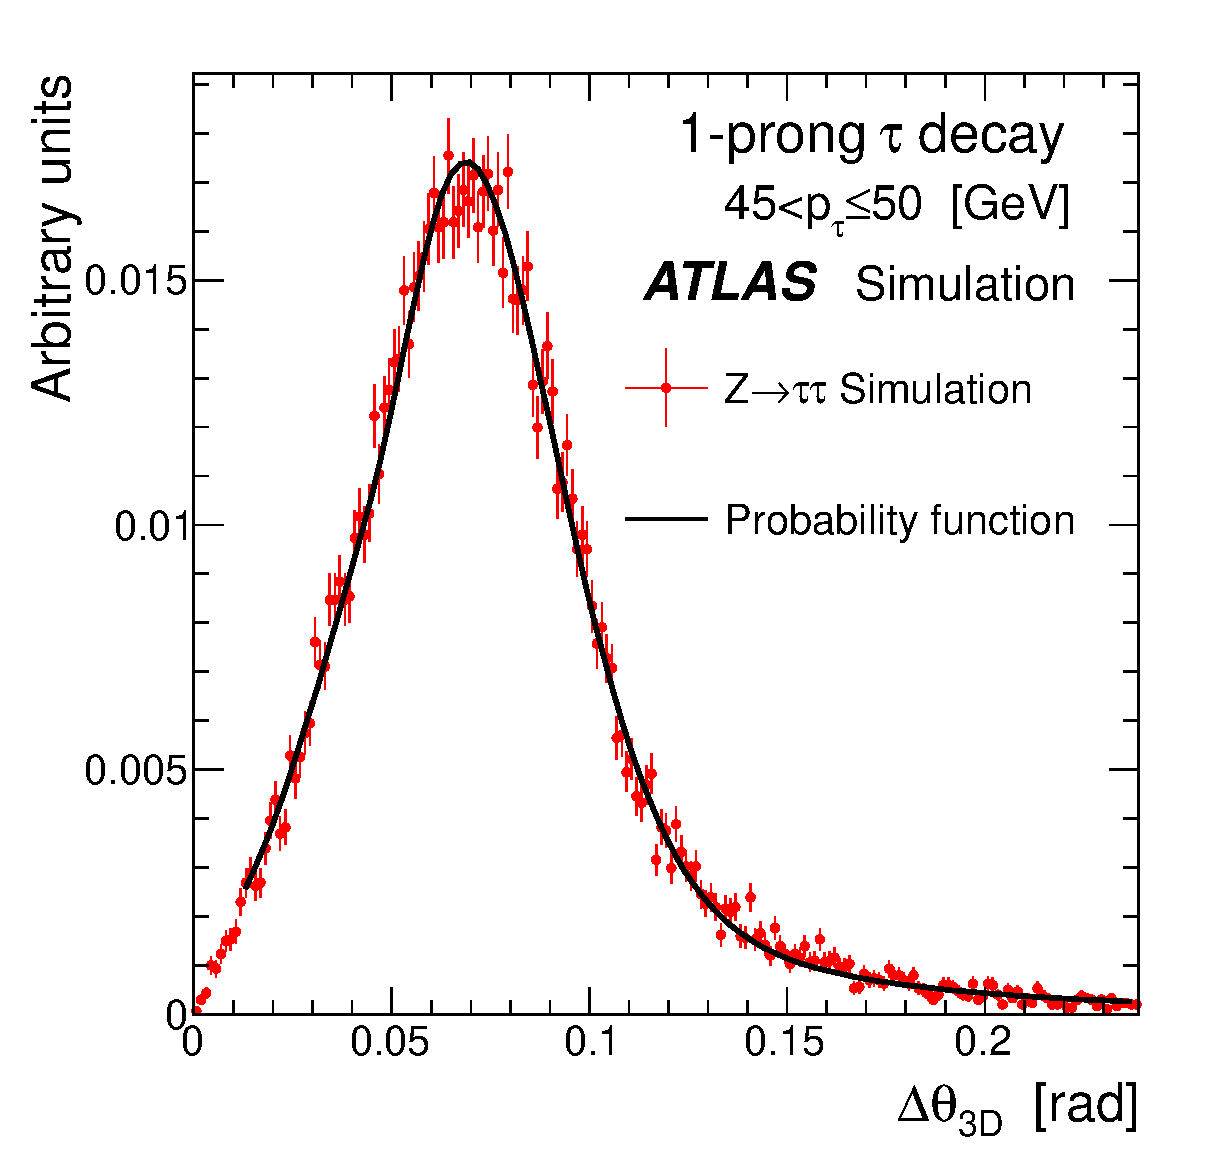
\includegraphics[width=0.32\textwidth]{figures/ATLAS-CONF-2011-132/fig_01b}
  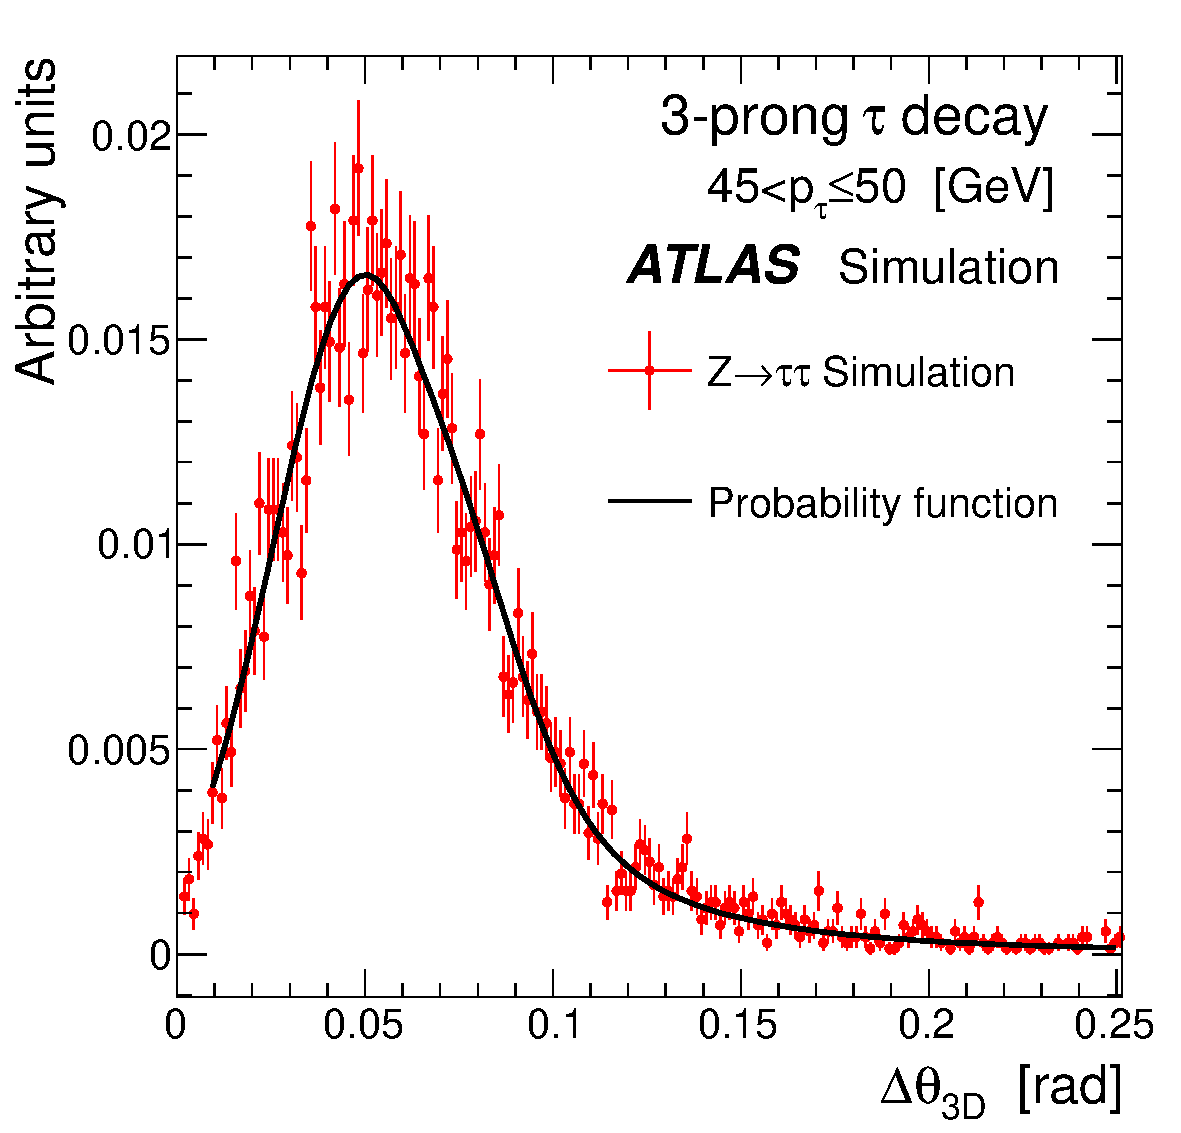
\includegraphics[width=0.32\textwidth]{figures/ATLAS-CONF-2011-132/fig_01c}
  \caption{Input assumptions of the angle between the visible and invisible tau lepton decay products, for leptonic decays (left), 1-track hadronic decays (center), and 3-track hadronic decays (right)~\cite{ATLAS-CONF-2011-132}.}
  \label{fig:strategy-mtautau-inputs}
\end{figure}

A similar technique, named \textsc{SVFit}, is used in the CMS $\Htautau$ analysis~\cite{2014.cms-htautau}.

\subsection{Performance}
\label{sec:strategy-mtautau-performance}

The reconstructed $\mMMC$ is shown in the $\tautaulh$ boosted and VBF categories in \cref{fig:strategy-mtautau-raw}. Good separation is observed for $\Ztautau$ and $\Htautau$. For both processes, the efficiency for the MMC algorithm to converge is 99\%.

\begin{figure}[tp]
  \centering
  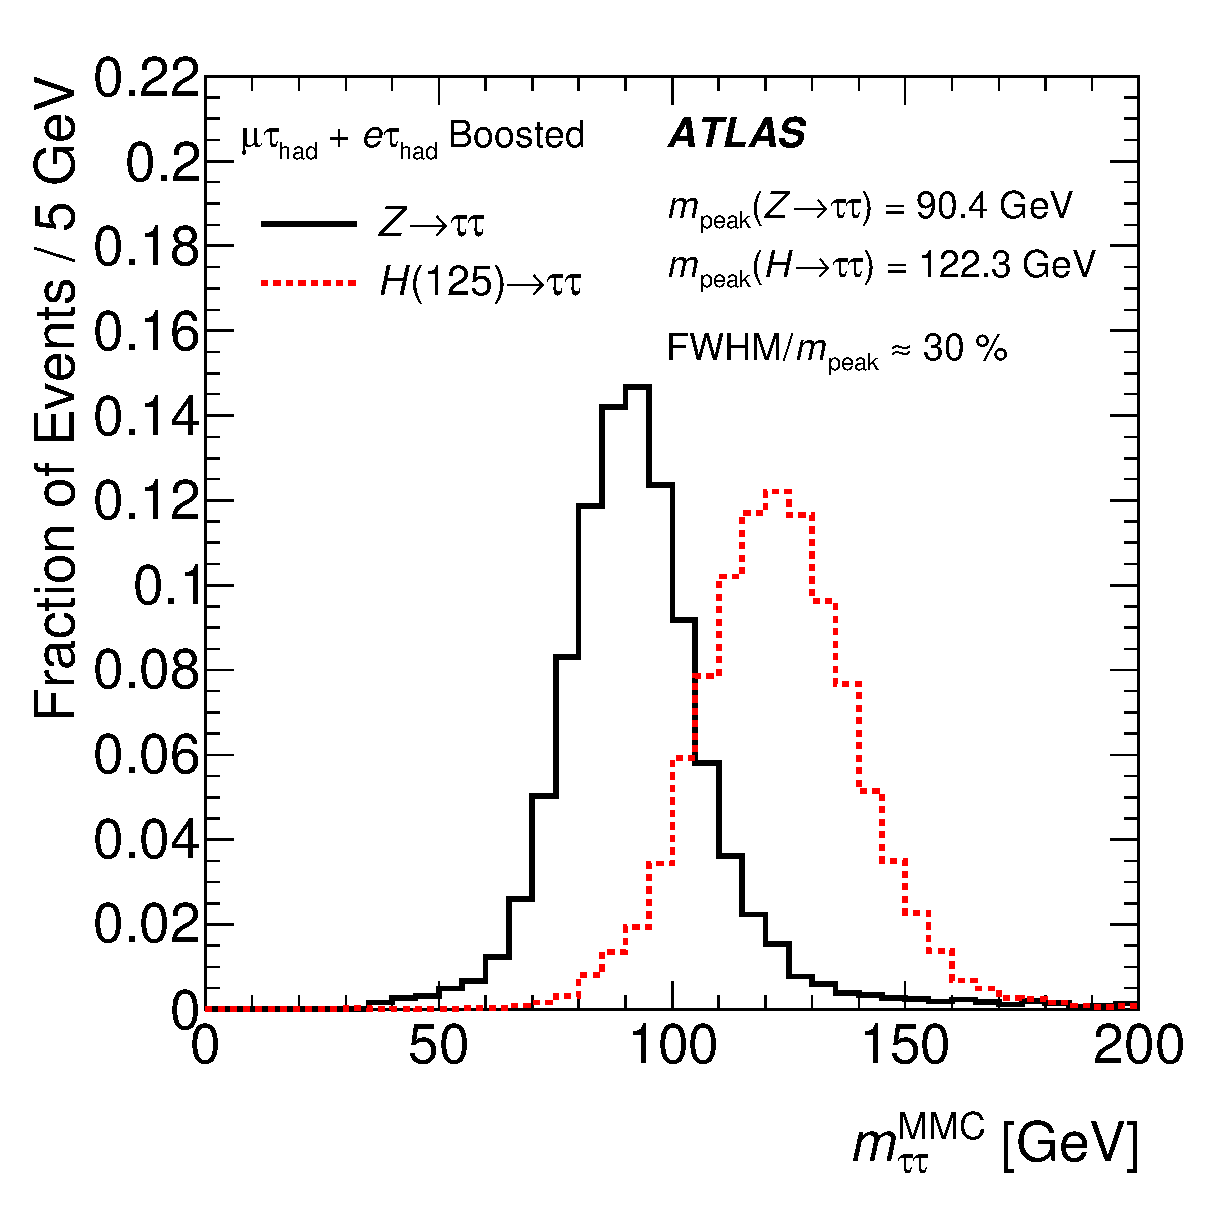
\includegraphics[width=0.48\textwidth]{figures/HIGG-2013-32/fig_01b}
  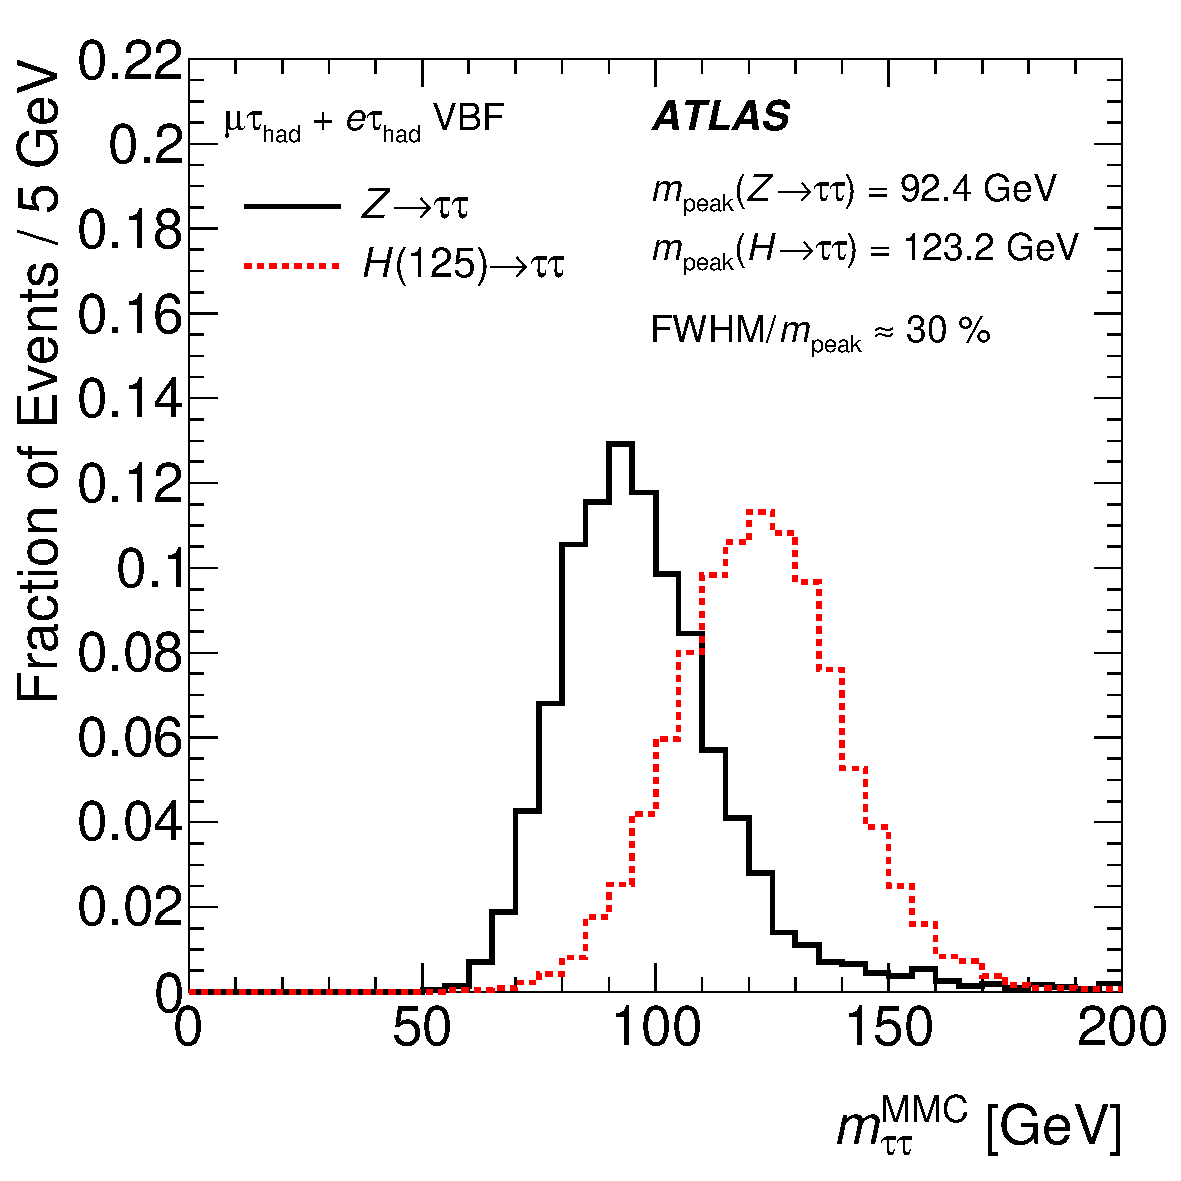
\includegraphics[width=0.48\textwidth]{figures/HIGG-2013-32/fig_01a}
  \caption{Predicted distributions of $\mtautau$ for $\Ztautau$ and $\Htautau$ for the MMC reconstruction algorithm in the boosted category (left) and VBF category (right).}
  \label{fig:strategy-mtautau-raw}
\end{figure}

To compare the performance of the various $\mtautau$ reconstruction techniques, the efficiency for a requirement $\mtautau > X$ is calculated across the mass range for $\Htautau$ (signal) and $\Ztautau$ (background). An ideal $\mtautau$ algorithm would have $\epsilon(\Htautau)$ near 1 and $\epsilon(\Ztautau)$ near 0 for $\mtautau > 100, 110, 120$ GeV. The efficiencies are shown in \cref{fig:strategy-mtautau-ROC} in the boosted and VBF categories. The distributions of the various $\mtautau$ algorithms are shown in \cref{apx:mtautau}.

\begin{figure}[tp]
  \centering
  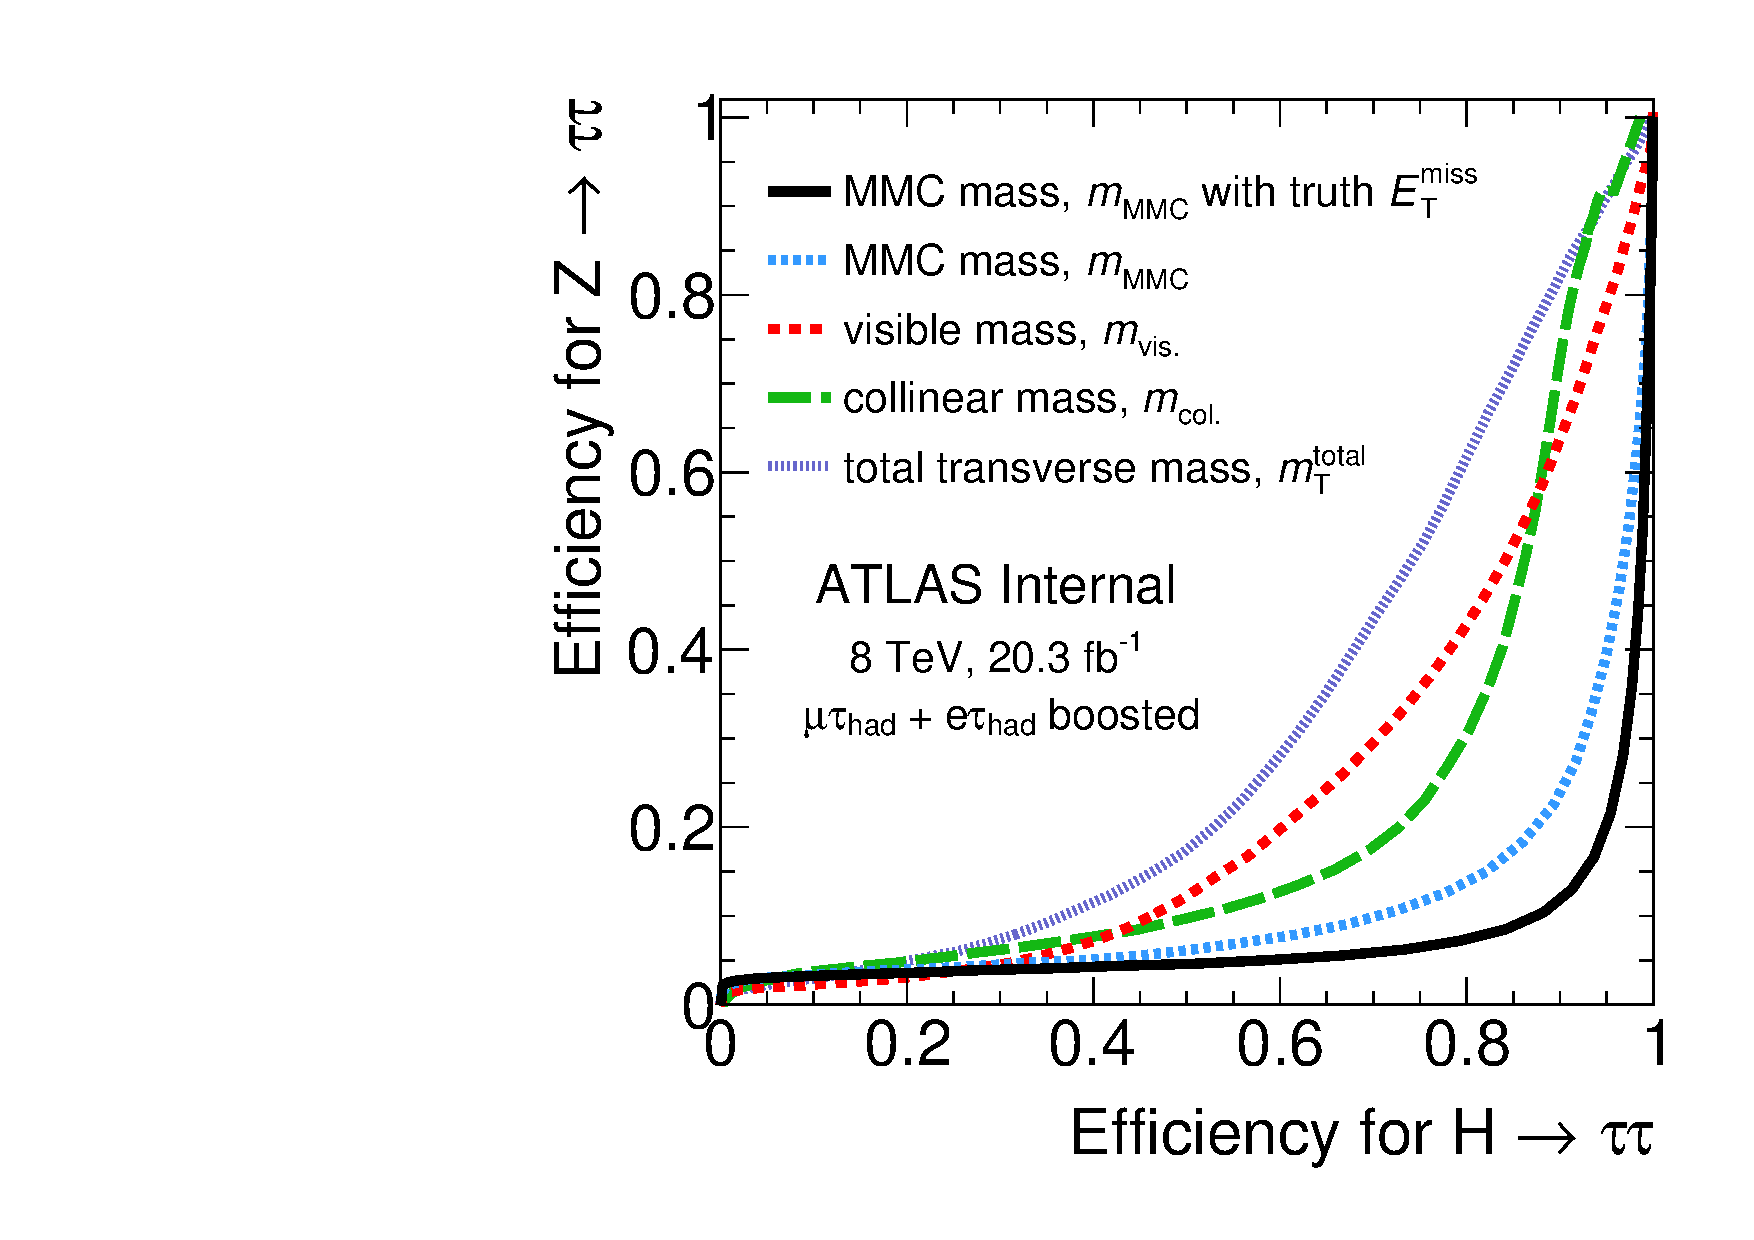
\includegraphics[width=0.48\textwidth]{figures/mtautau/mtautau-boost}
  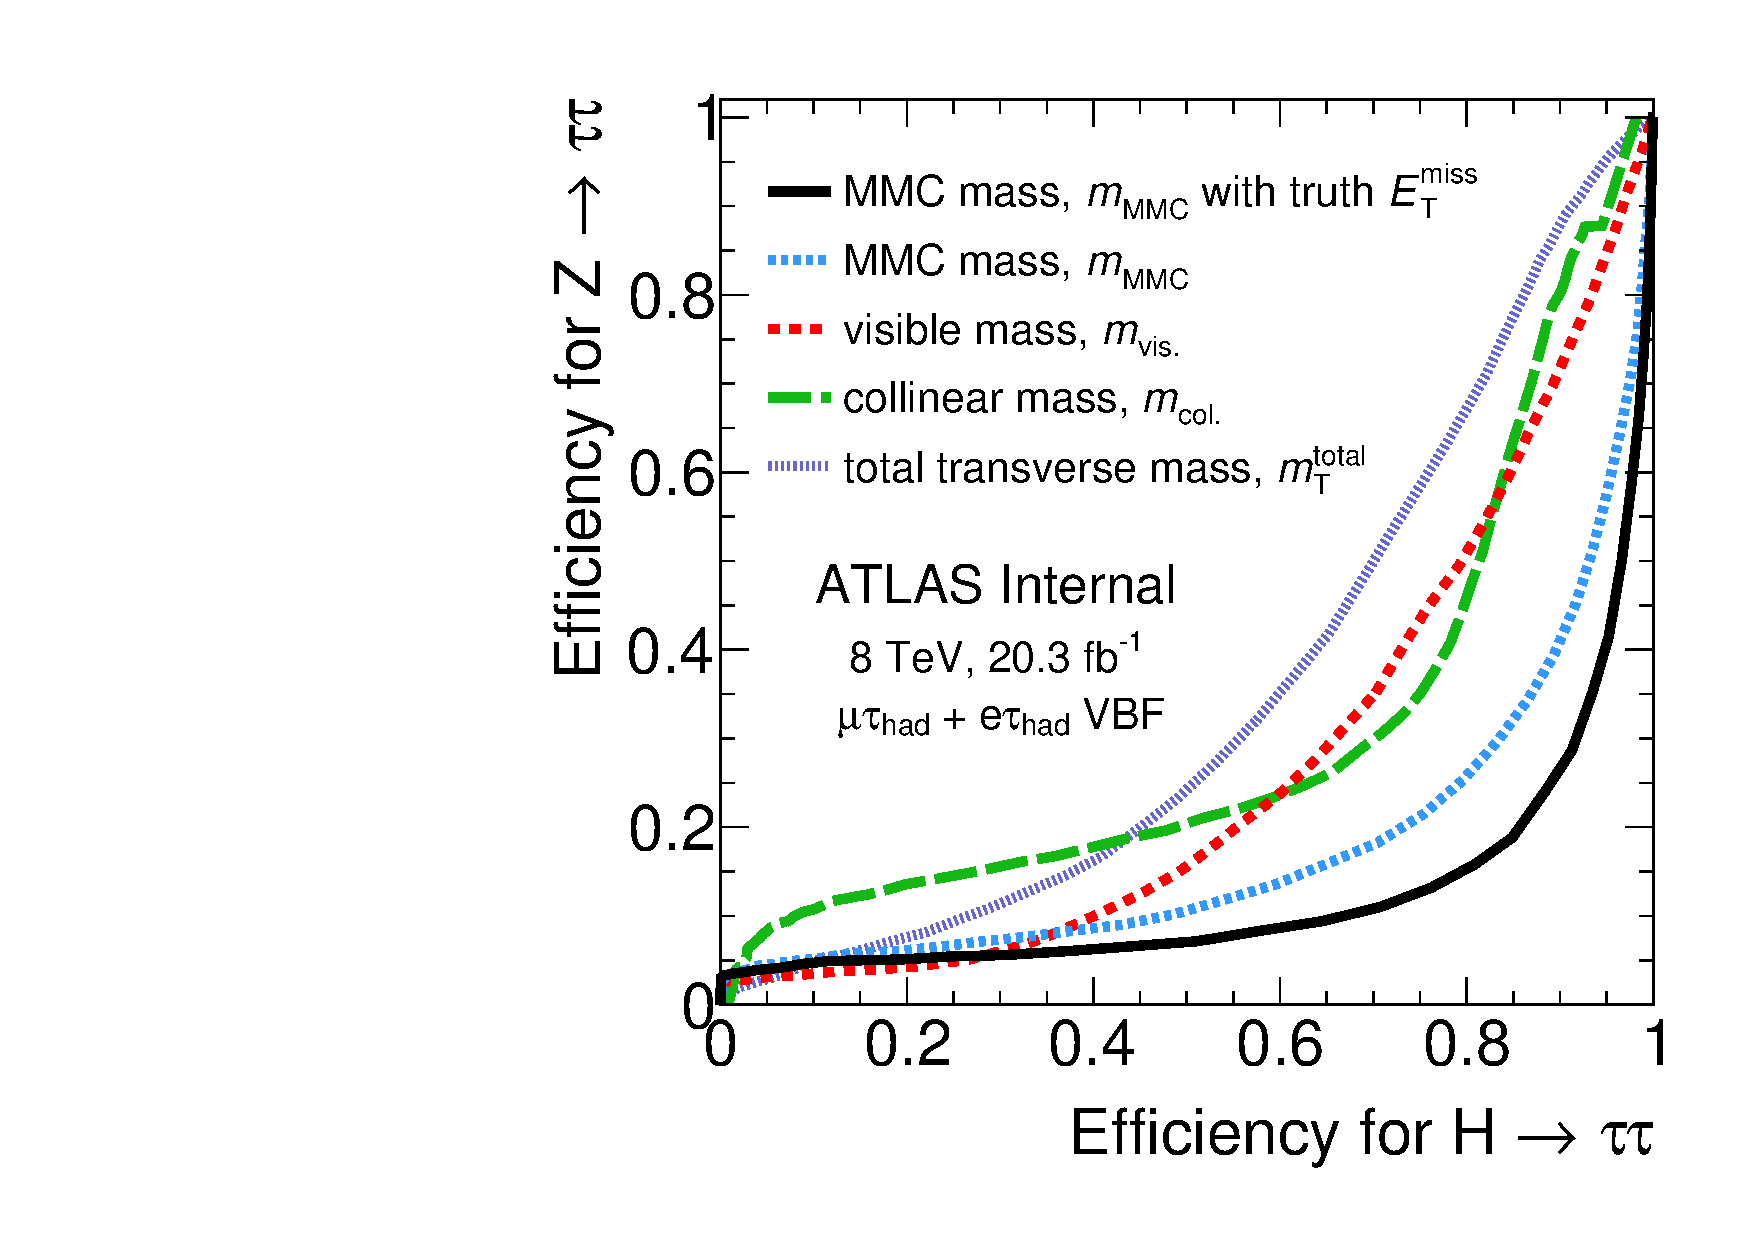
\includegraphics[width=0.48\textwidth]{figures/mtautau/mtautau-vbf}
  \caption{Efficiency for $\Htautaulh$ versus the efficiency for $\Ztautaulh$ for various $\mtautau$ reconstruction algorithms in the boosted category (left) and VBF category (right).}
  \label{fig:strategy-mtautau-ROC}
\end{figure}

Of the $\mtautau$ algorithms considered, the MMC has the best performance in this metric. The $\MET$ reconstruction performance is among the limiting factors of the MMC algorithm.

\section{MVA discrimination}
\label{sec:strategy-mva}

The Higgs discovery program is driven by final states where the reconstructed Higgs mass is the most powerful variable for discriminating signal from background. This is especially true of the $\Hyy$ and $\HZZ$ analyses, where $m_H$ can be fully reconstructed and no nearby resonant backgrounds exist.

The landscape is not as easy for $\Htautau$. The resonant and irreducible $\Ztautau$ process is nearby in mass, and the resolution of the $\mtautau$ is similar to the difference between the masses due to the presence of neutrinos in the tau lepton decays. Additionally, the distinctive VBF signature provides potentially greater discriminating power than $\mtautau$.

For these reasons, a multi-variate (MVA) analysis is chosen where event-level observables like $\mMMC$ and $\mjj$ are input to a boosted decision tree (BDT) discriminator~\cite{1984.decision-trees,2004.bdts-miniboone}. The BDT attempts to classify a given event as signal-like or background-like with a continuous output score judged on the multi-dimensional evaluation of input variables. A score of 1 is most signal-like, and a score of -1 is most background-like.

\subsection{Inputs}
\label{sec:strategy-mva-inputs}

Inputs to the VBF BDT discriminator can be broadly grouped into two classes: $\Htautau$ kinematics and VBF kinematics. $\Htautau$ kinematics provide discrimination against non-$\Htautau$ decays: for example, the $\mMMC$ discriminates against all backgrounds, and the transverse $W$-mass $\mT$ discriminates against $\Wjets$ events. VBF kinematics provide discrimination against non-VBF produced processes: for example, dijets produced in VBF tend to have larger $\mjj$ than QCD $\Ztautau$ produced in association with two jets. One of the appealing features of the BDT, however, is that correlations between these groups of variables are exploited in the classification. This is discussed in more detail in \cref{sec:strategy-mva-correlations}.

An interesting sub-set of inputs are centrality variables. These are transformations of discrete properties to continuous observables. The first, $\MET$ $\phi$-centrality, quantifies whether the $\MET$ is between the lepton and $\tauh$ in the transverse plane. In $\tautau$ systems, the $\MET$ typically points between the lepton and $\tauh$, whereas non-$\tautau$ systems have no such constraint. The $\MET$ $\phi$-centrality is accordingly maximized when the $\MET$ points directly between the lepton and $\tauh$ and miminized when it points opposite.

The second centrality varible, lepton $\eta$-centrality, quantifies whether the lepton is between the VBF jets in $\eta$. In VBF systems, the Higgs decay products typically point between the VBF jets in $\eta$, whereas non-VBF systems have no such constraint. Visualization of the allowed values of the centralities are shown in \cref{fig:strategy-centrality-cartoons}.

\begin{figure}[tp]
  \centering
  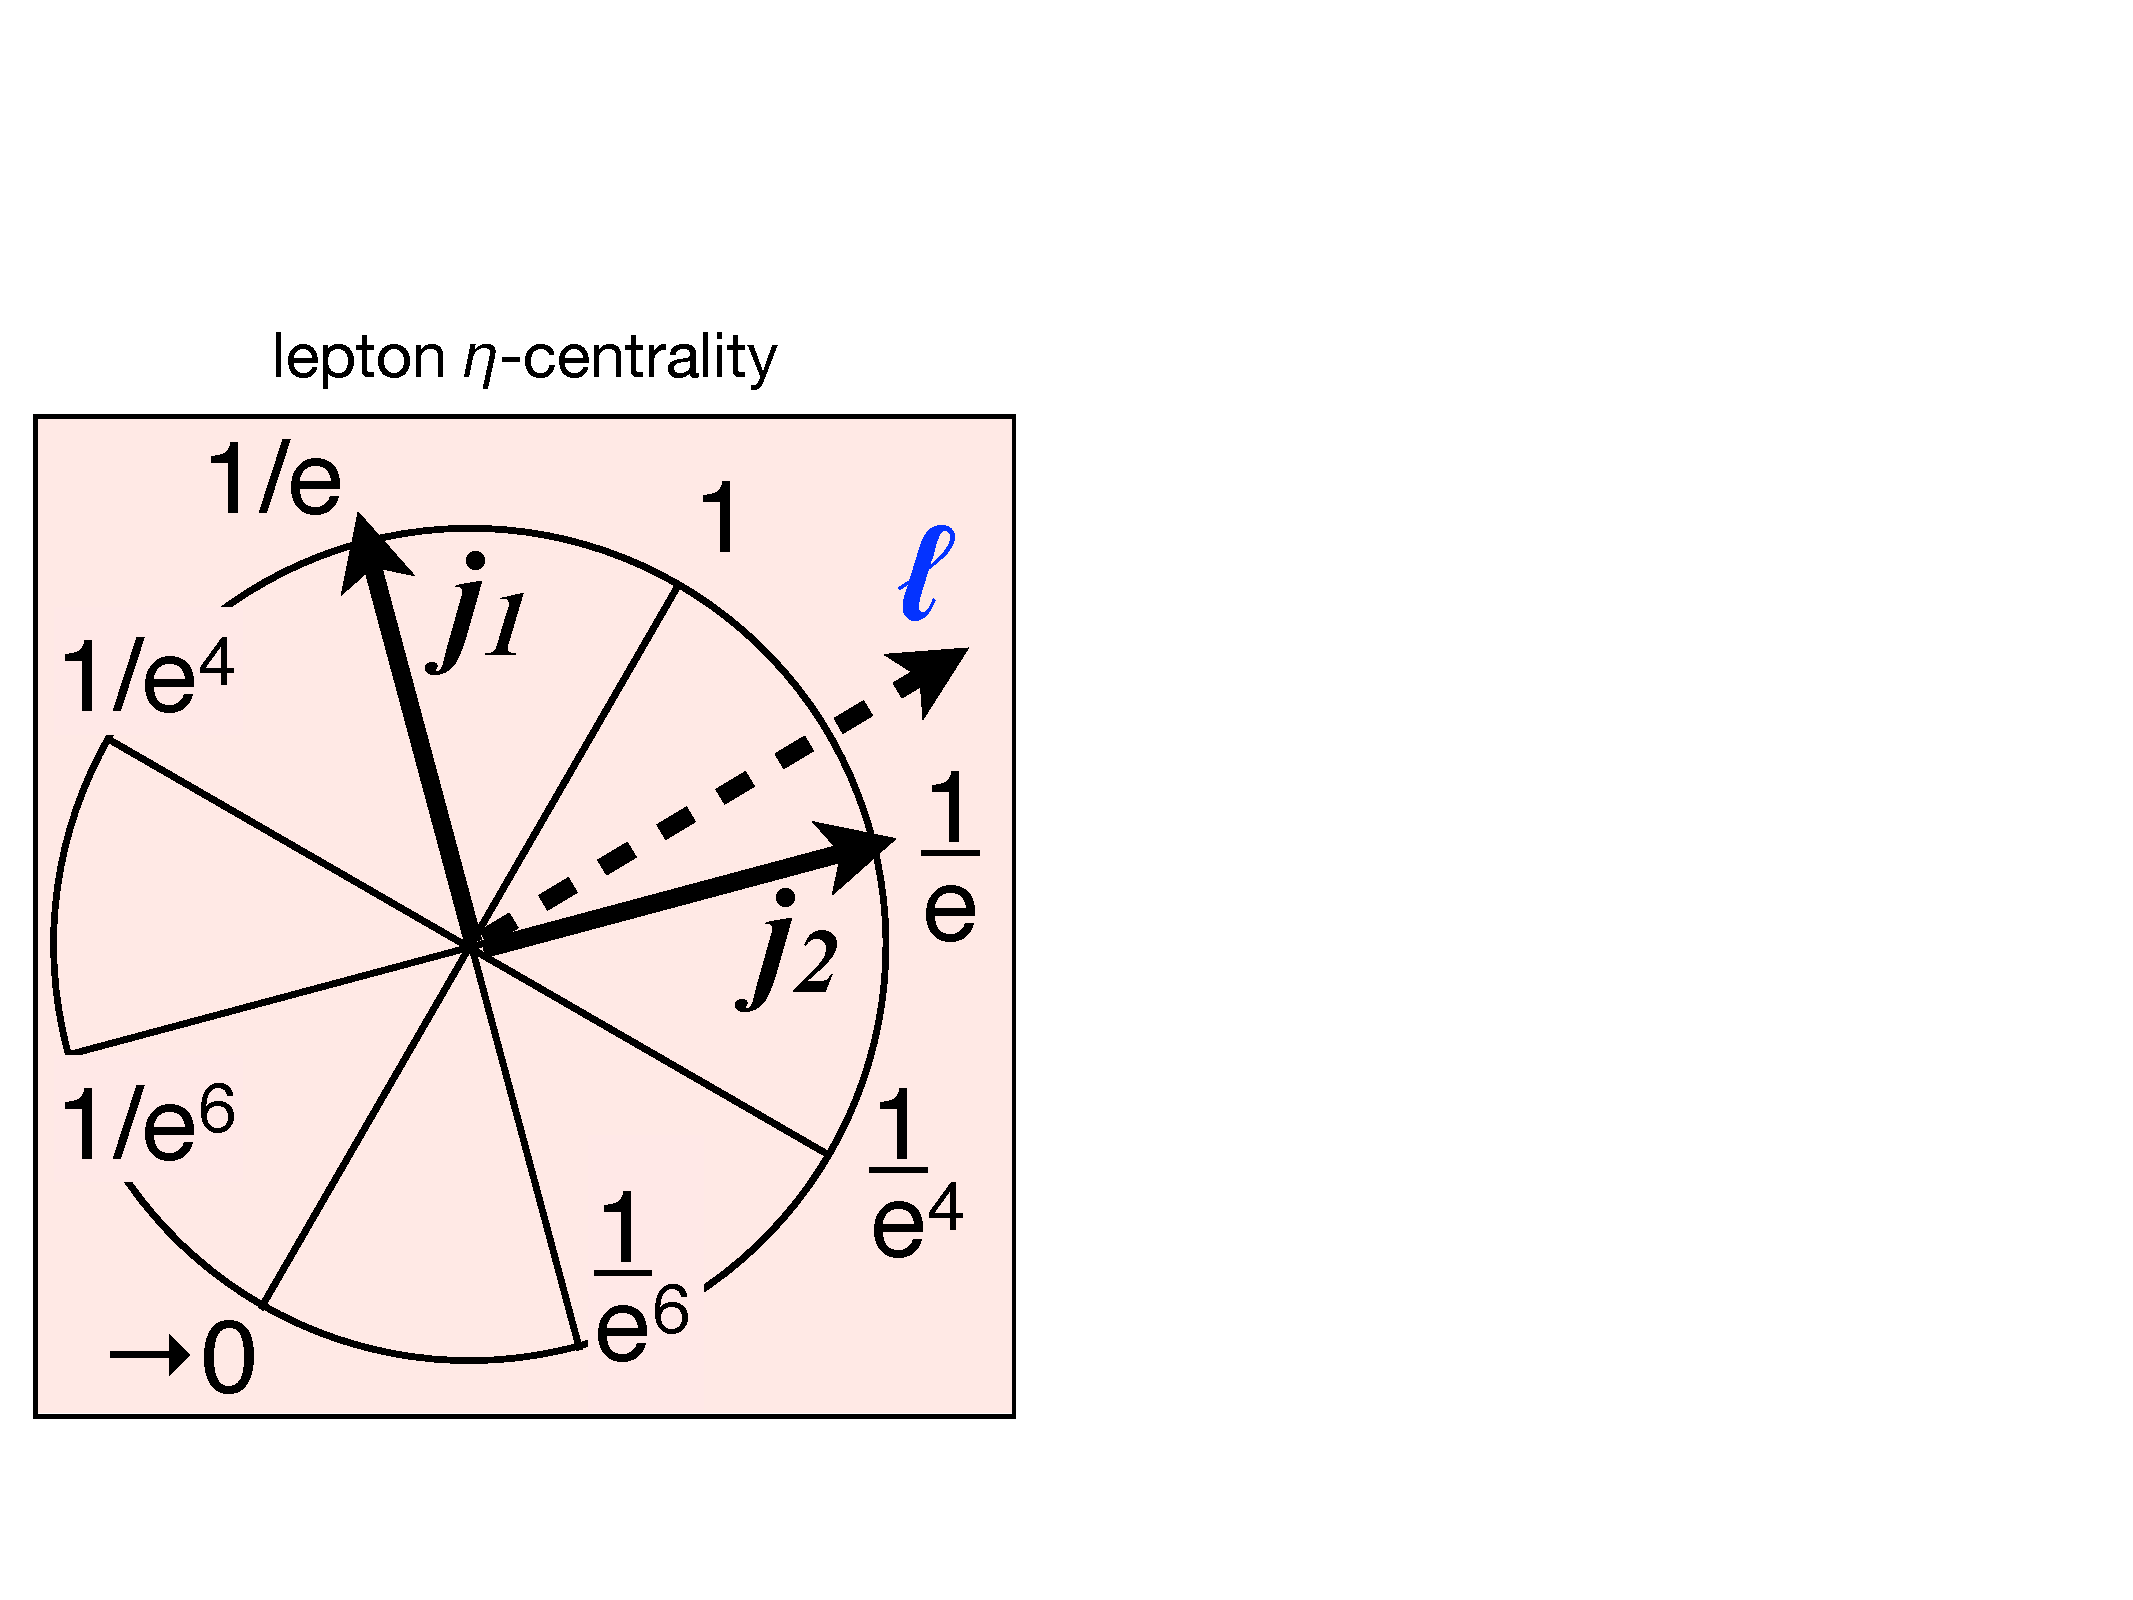
\includegraphics[width=0.48\textwidth]{figures/backgrounds/cartoon_lepton_eta_centrality}
  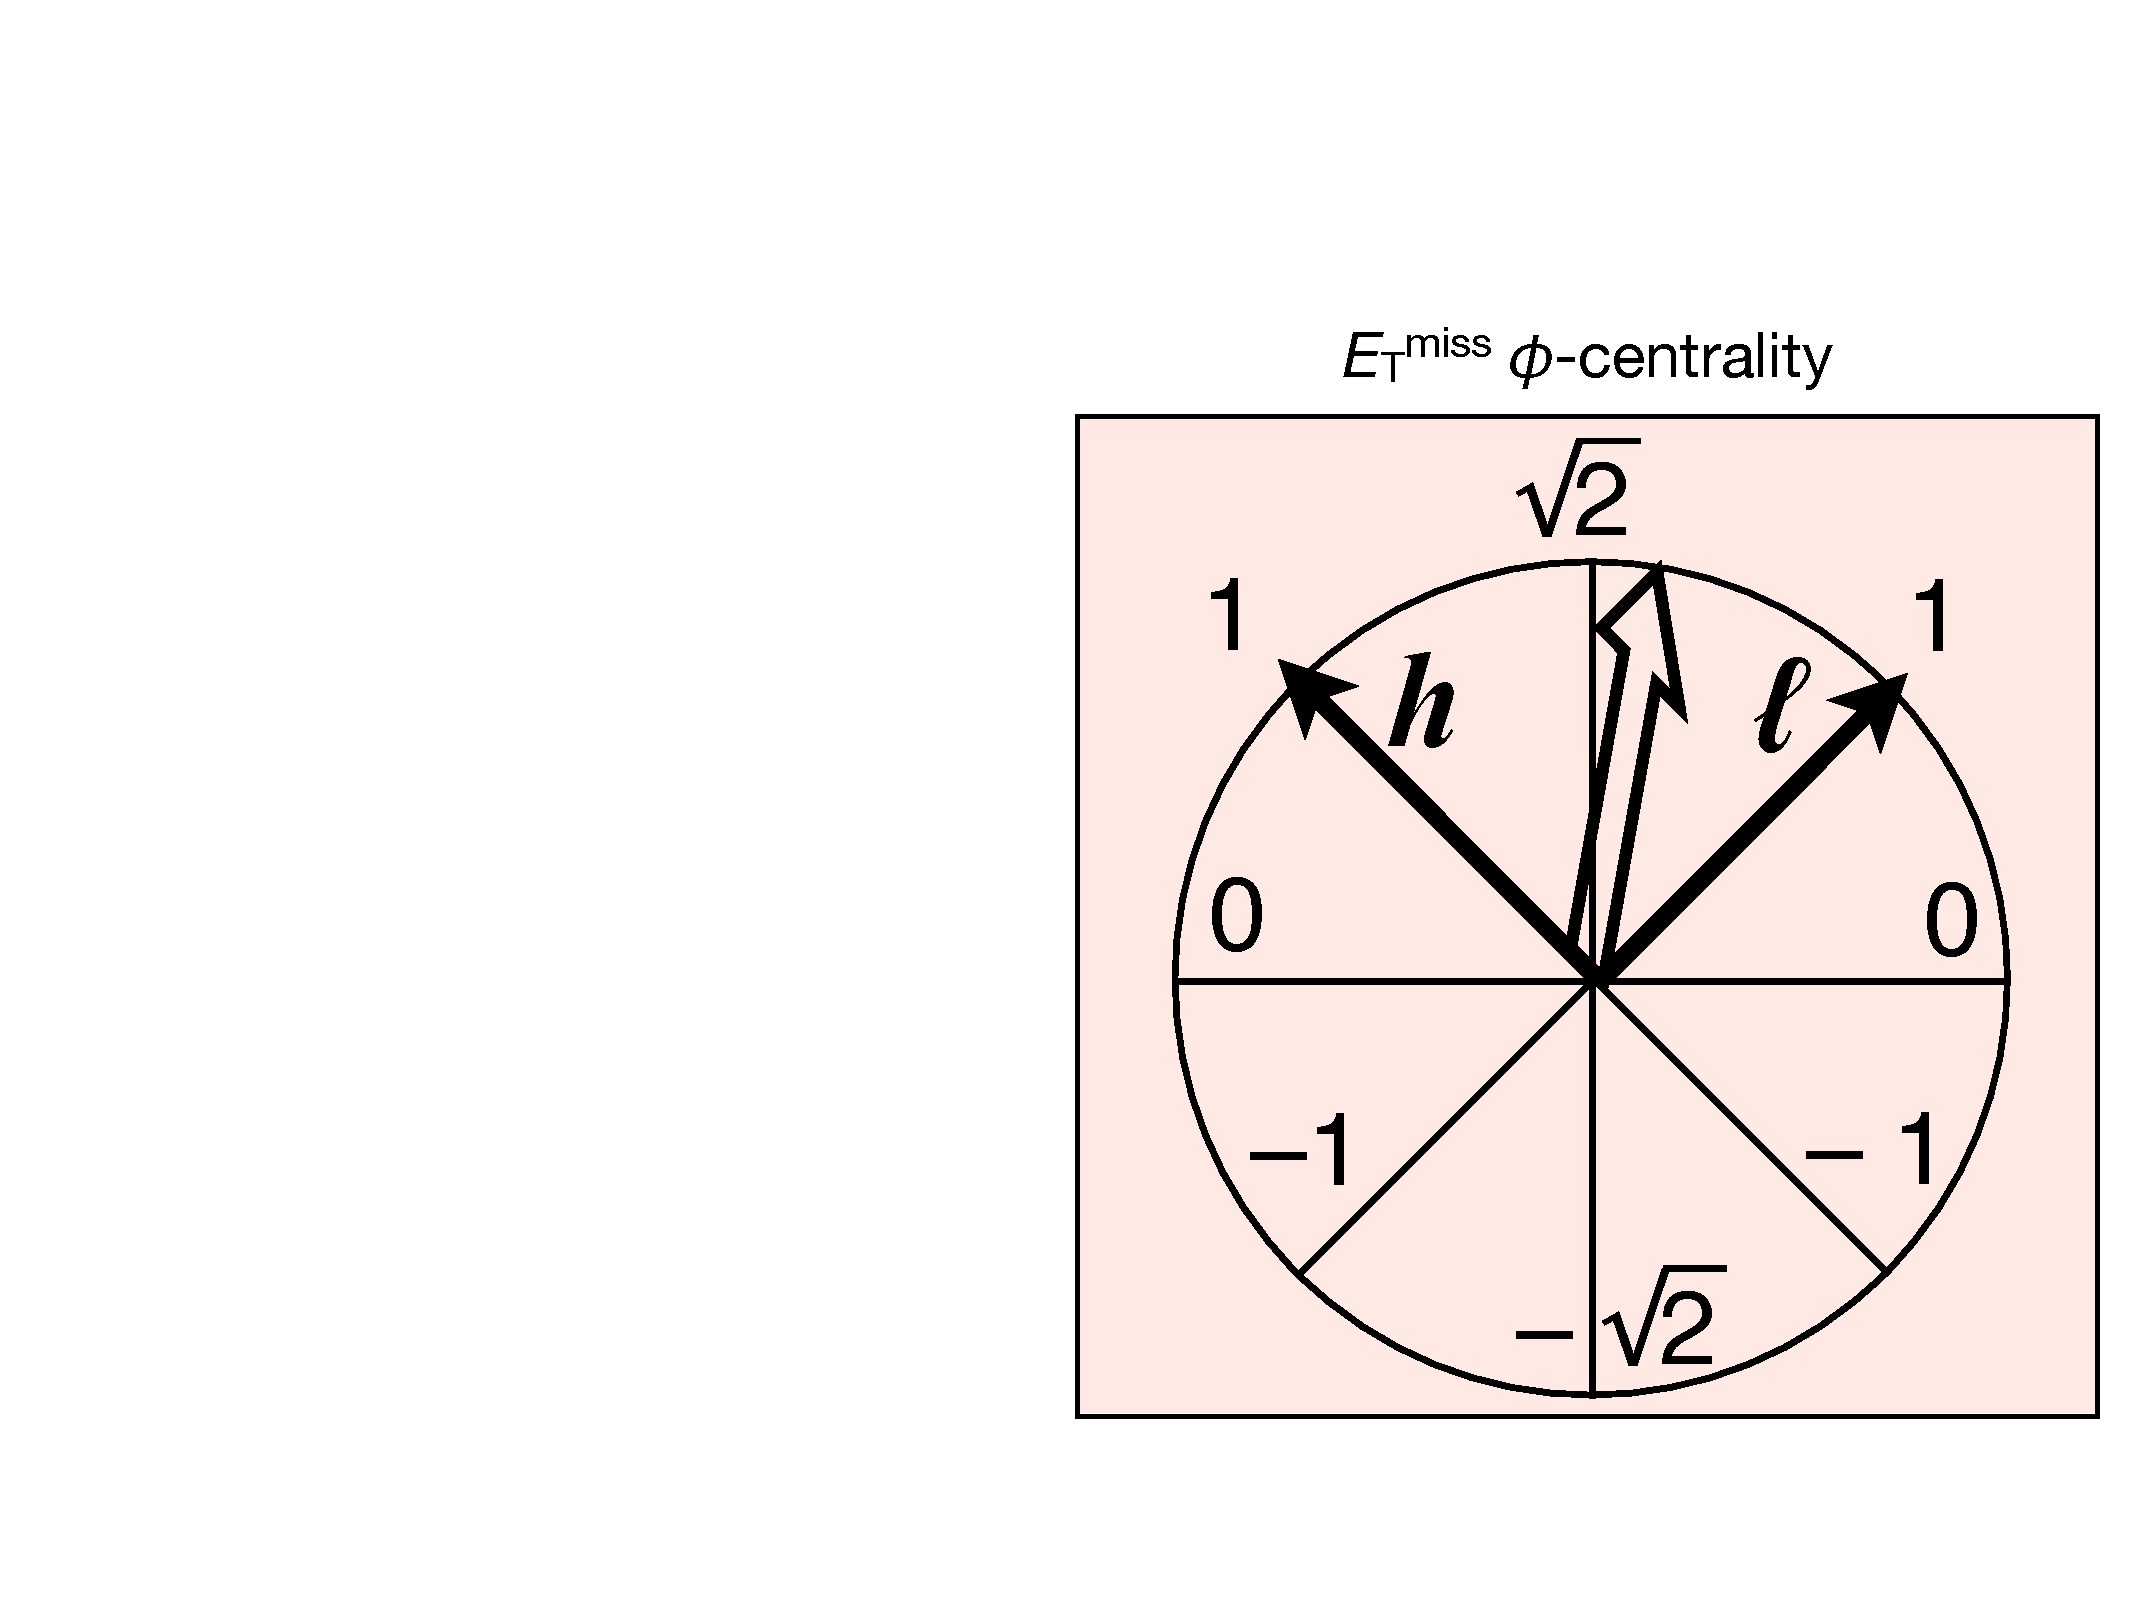
\includegraphics[width=0.48\textwidth]{figures/backgrounds/cartoon_met_phi_centrality}
  \caption{Cartoons of lepton $\eta$-centrality (left) and $\MET$ $\phi$-centrality (right), courtesy of Tae Min Hong.}
  \label{fig:strategy-centrality-cartoons}
\end{figure}

The choice of variables is optimized to give good separation while keeping the number of inputs small and manageable. The set of inputs used in the $\Htautaulh$ categories is shown in \cref{tab:strategy-inputs}. Distributions of input variables and other kinematics are shown in \cref{fig:strategy-overlaid-boost-1,fig:strategy-overlaid-boost-2} for the boosted category and \cref{fig:strategy-overlaid-vbf-1,fig:strategy-overlaid-vbf-2} for the VBF category. Signal and background predictions are discussed in greater detail in \cref{chap:backgrounds}.

\begin{table}[bp]
  \centering
  \renewcommand{\arraystretch}{1.4}
  \caption{Input variables to the $\Htautaulh$ BDT discriminators in the boosted and VBF categories.}
  \begin{tabular}{c|c|c|c}
Variable      & VBF       & boosted   & Description \\ 
\hline
$\mMMC$       & $\bullet$ & $\bullet$ & ditau mass \\
$\dR$         & $\bullet$ & $\bullet$ & spatial separation of lepton, $\tauh$ \\
$\metphicent$ & $\bullet$ & $\bullet$ & $\phi$-centrality of $\MET$ between lepton, $\tauh$ \\
$\mT$         & $\bullet$ & $\bullet$ & transverse $W$ mass\\
$\deta$       & $\bullet$ &           & $\eta$-separation of VBF jets \\
$\mjj$        & $\bullet$ &           & mass of VBF jets \\
$\etaprod$    & $\bullet$ &           & $\eta$-product of VBF jets \\ 
$\pttot$      & $\bullet$ &           & vector sum of lepton, $\tauh$, $\MET$ and VBF jets \\
$\lepetacent$ & $\bullet$ &           & $\eta$-centrality of lepton between VBF jets \\
$\sumpt$      &           & $\bullet$ & scalar sum of lepton, $\tauh$, and all jets \\
$\ptratio$    &           & $\bullet$ & ratio of lepton $\pt$ to $\tauh$ $\pt$ \\
\end{tabular}


  \label{tab:strategy-inputs}
\end{table}

% boost
% ---------------------------------------------------------------------------------
\clearpage
\begin{figure}[tp]
  \centering
  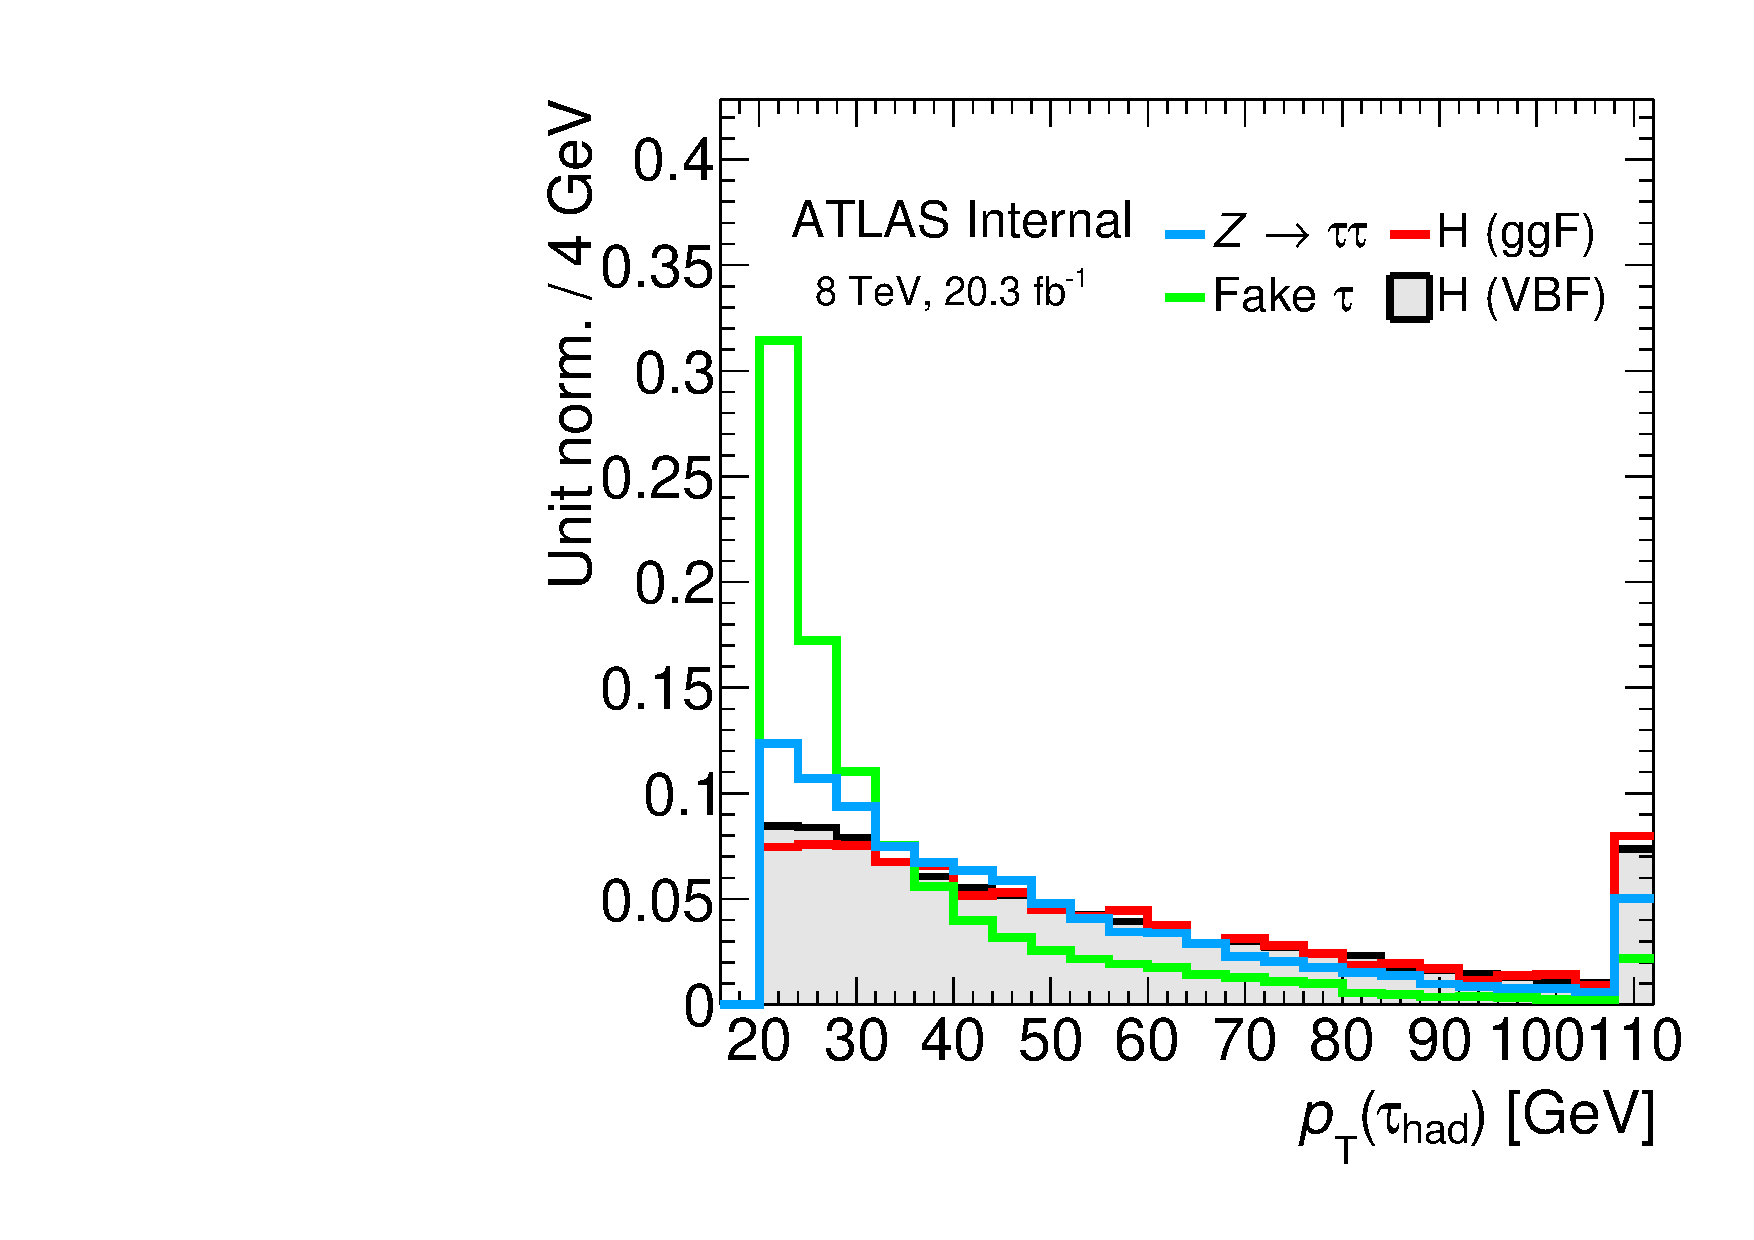
\includegraphics[width=0.32\textwidth]{figures/overlaid/boost/tau-pt}
  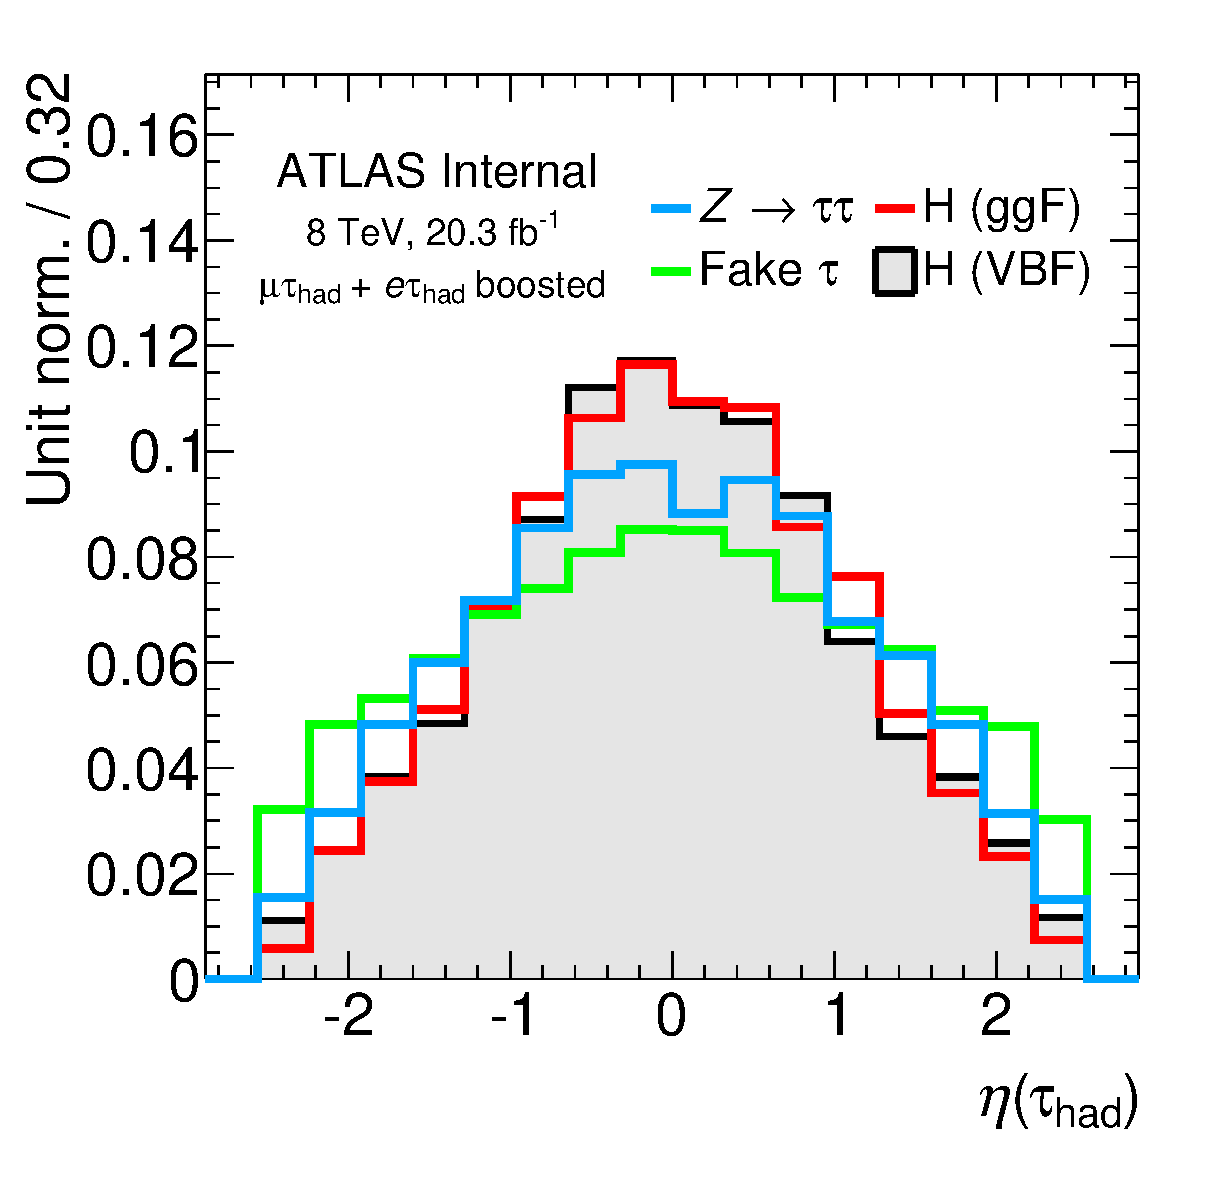
\includegraphics[width=0.32\textwidth]{figures/overlaid/boost/tau-eta}
  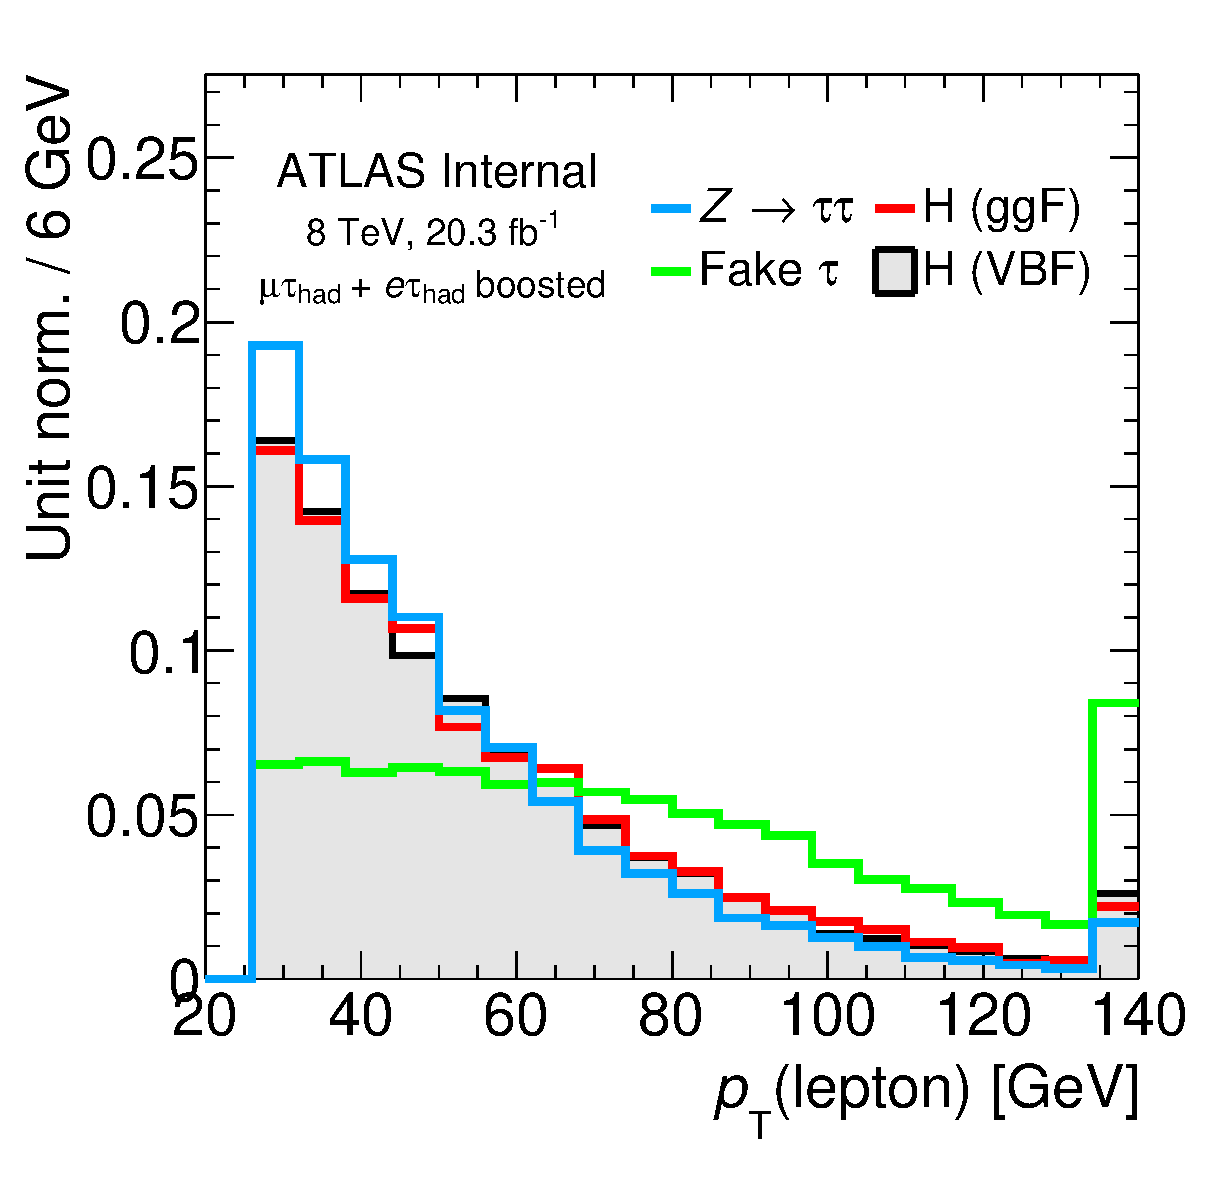
\includegraphics[width=0.32\textwidth]{figures/overlaid/boost/lep-pt-hi} \\
  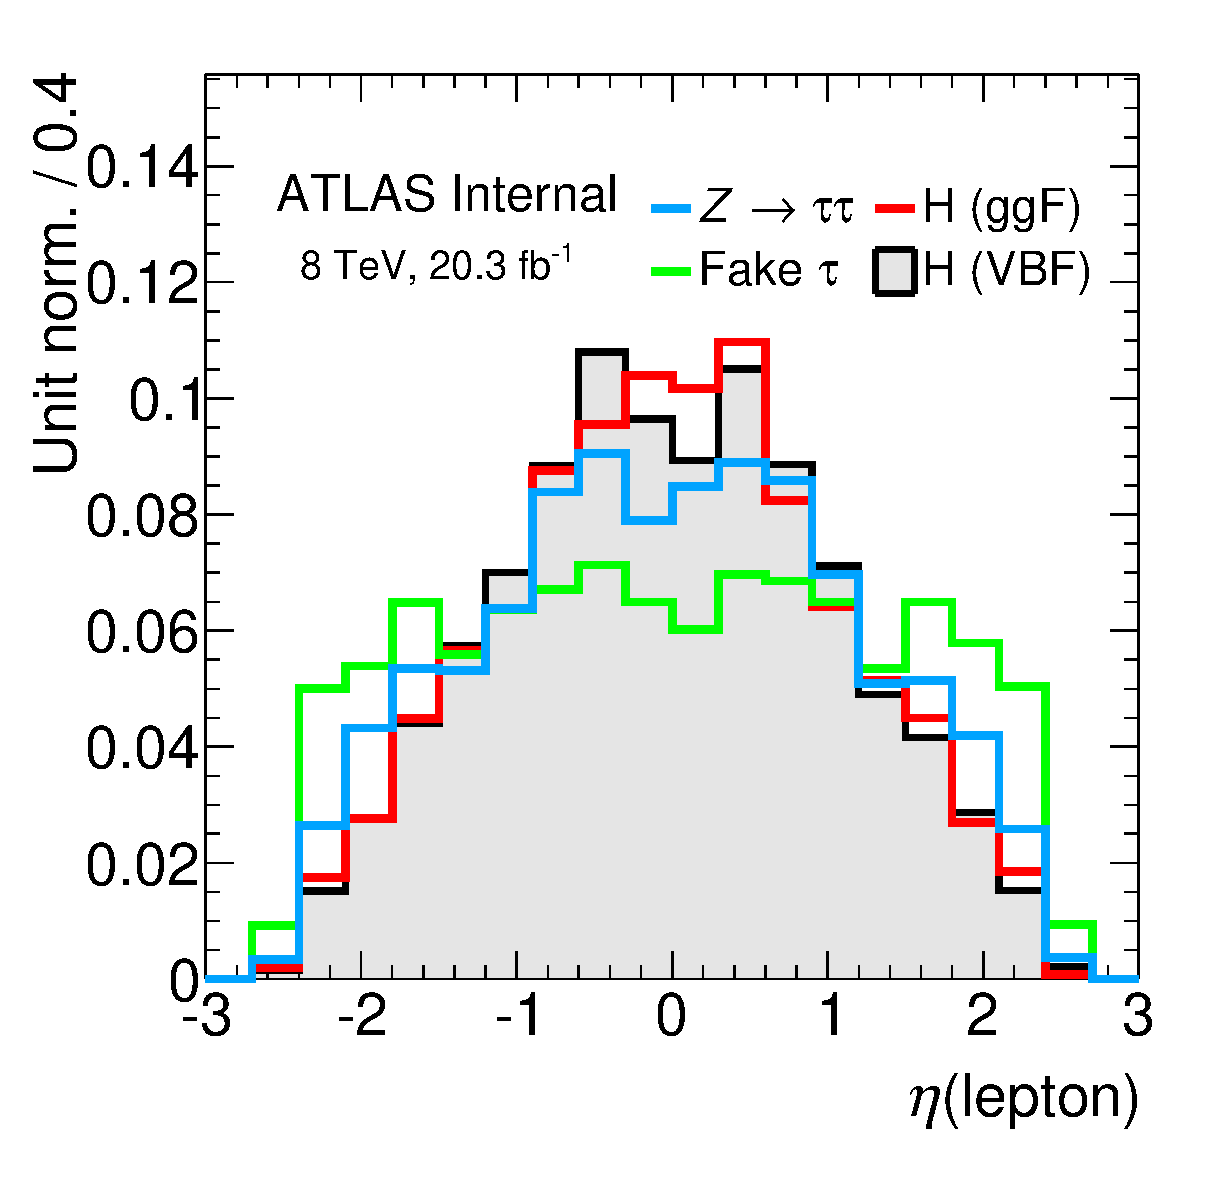
\includegraphics[width=0.32\textwidth]{figures/overlaid/boost/lep-eta} 
  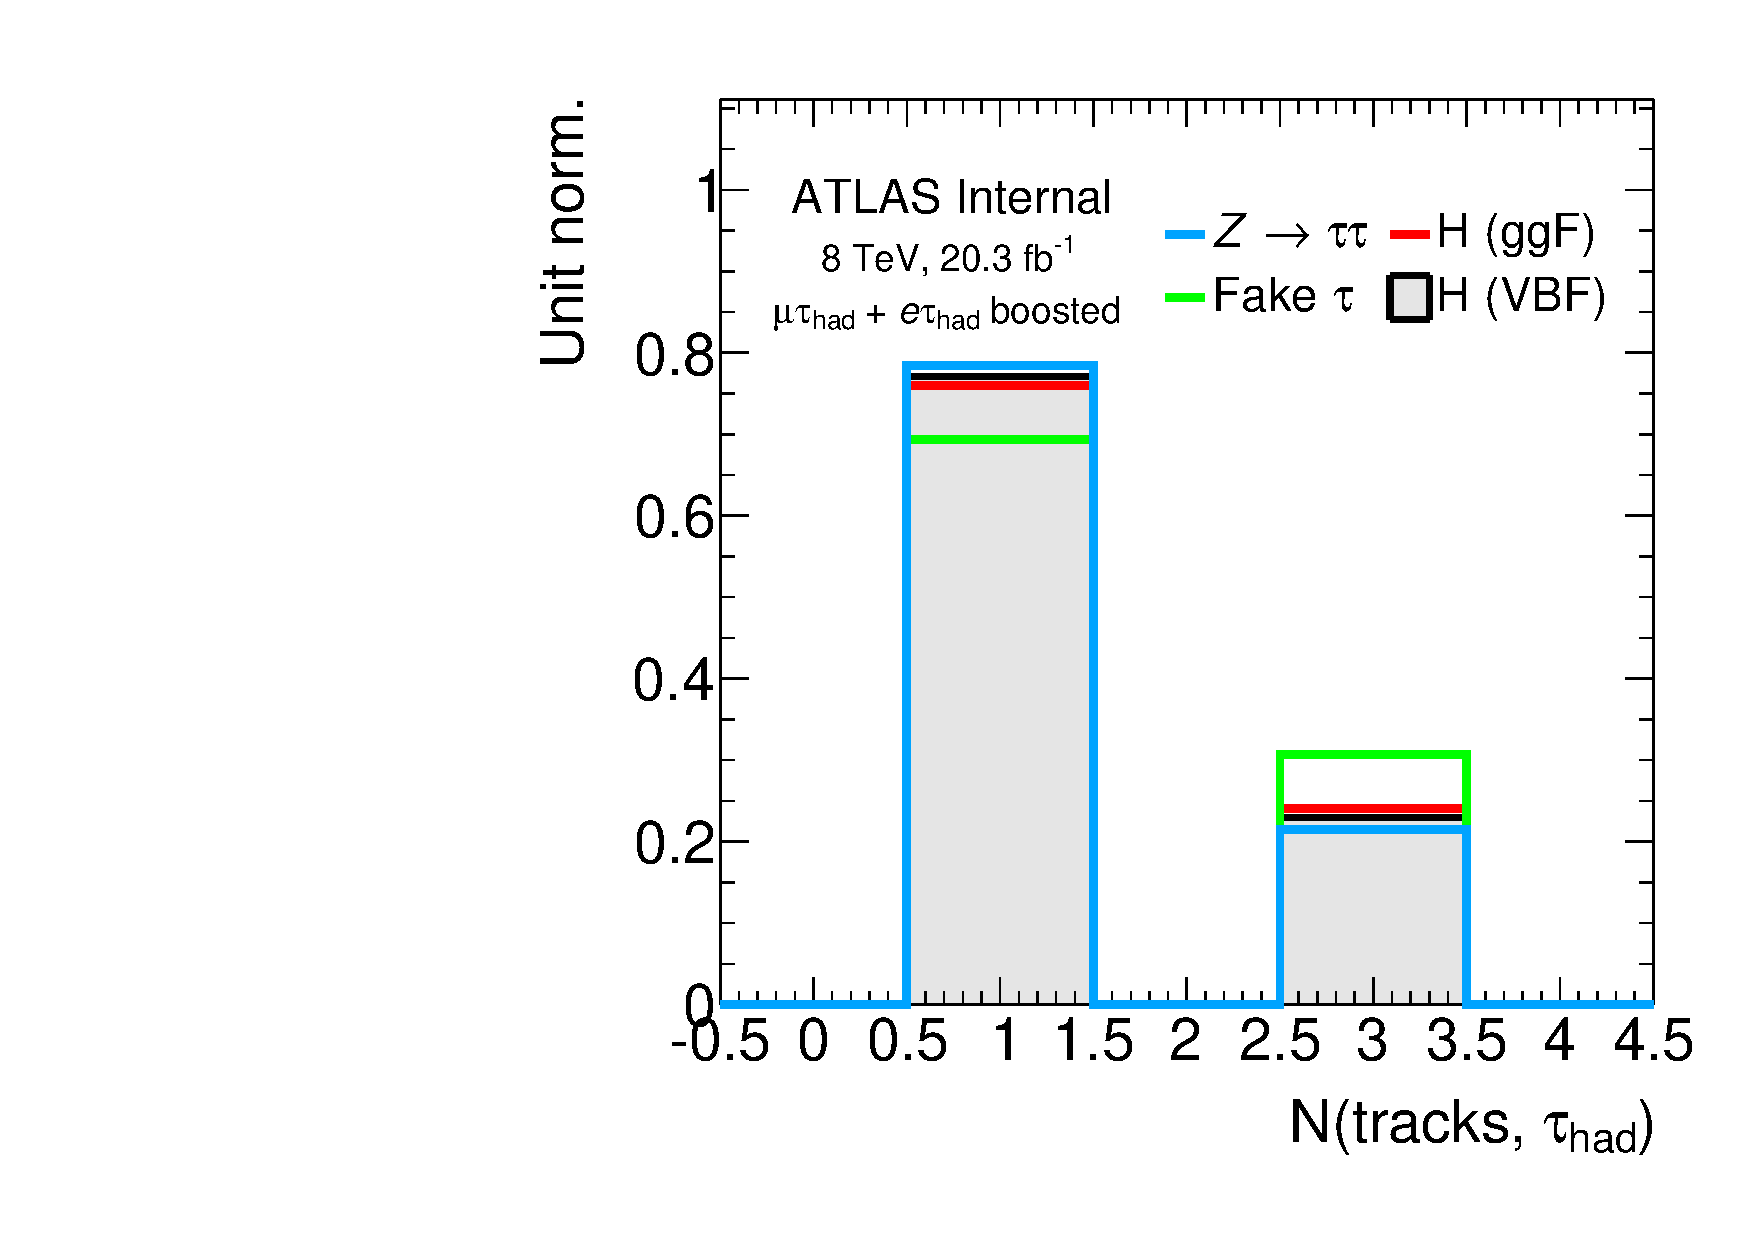
\includegraphics[width=0.32\textwidth]{figures/overlaid/boost/tau-numTrack}
  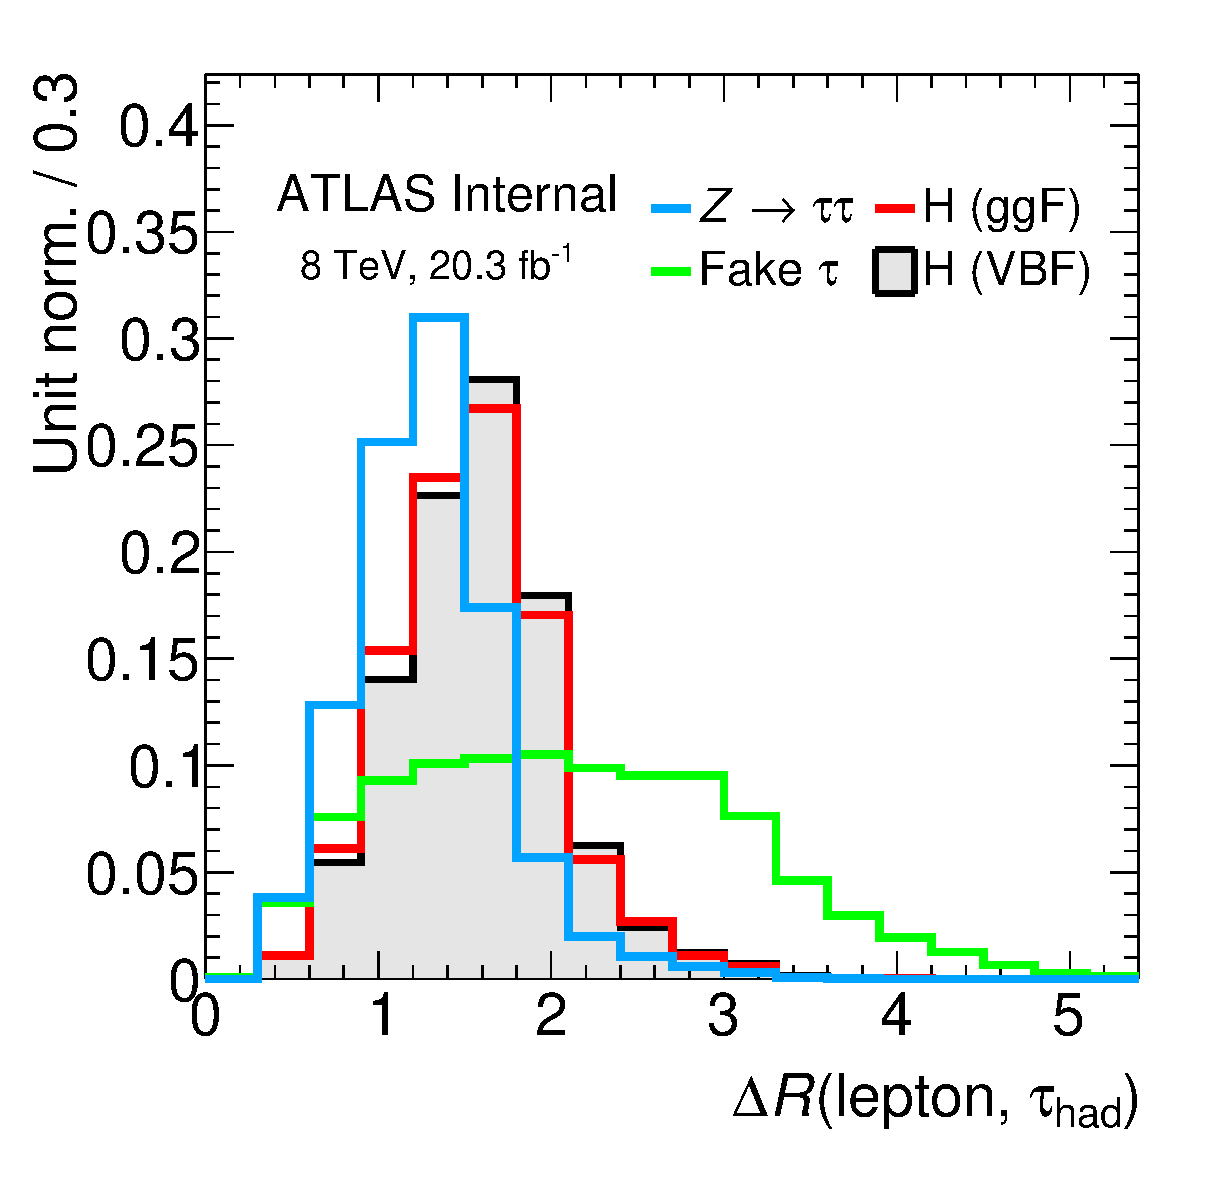
\includegraphics[width=0.32\textwidth]{figures/overlaid/boost/taulep-dR} \\
  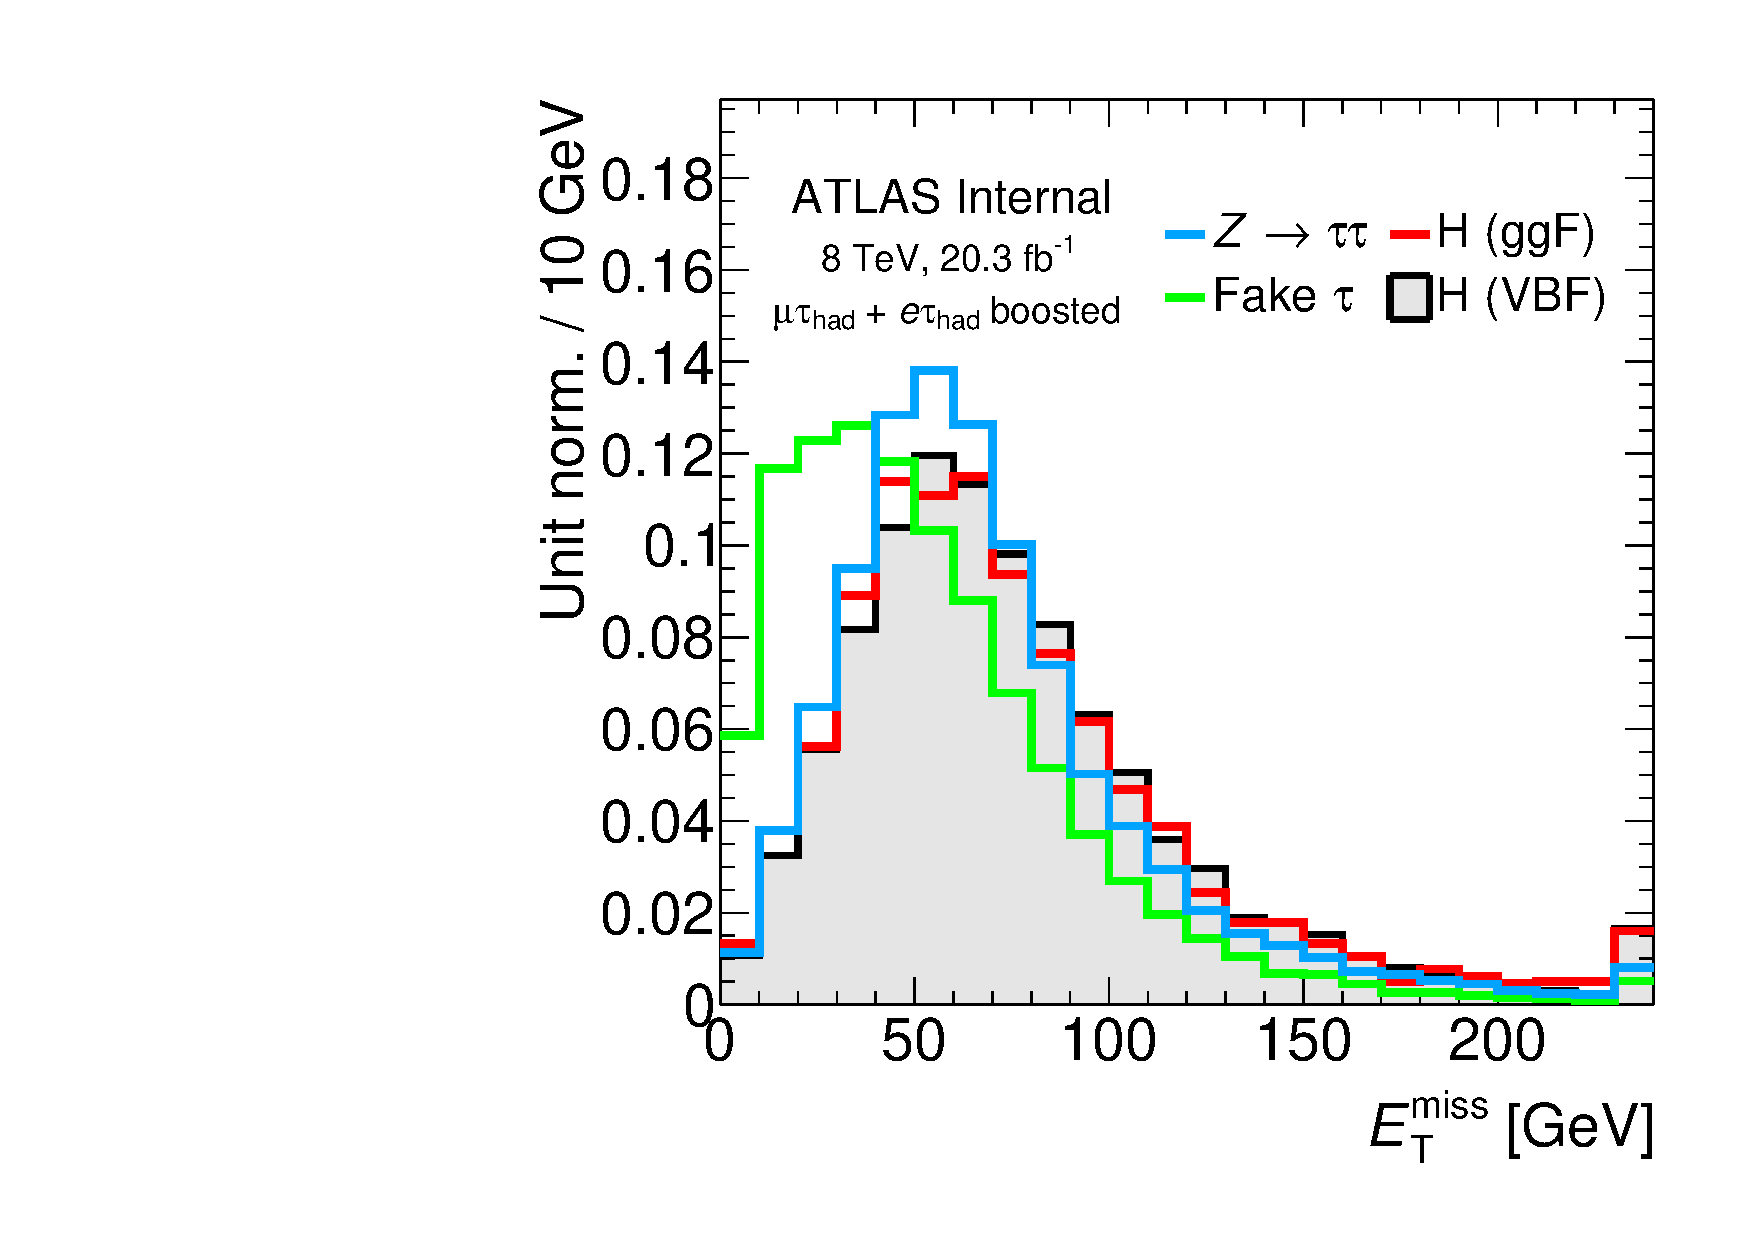
\includegraphics[width=0.32\textwidth]{figures/overlaid/boost/met-pt-hi}
  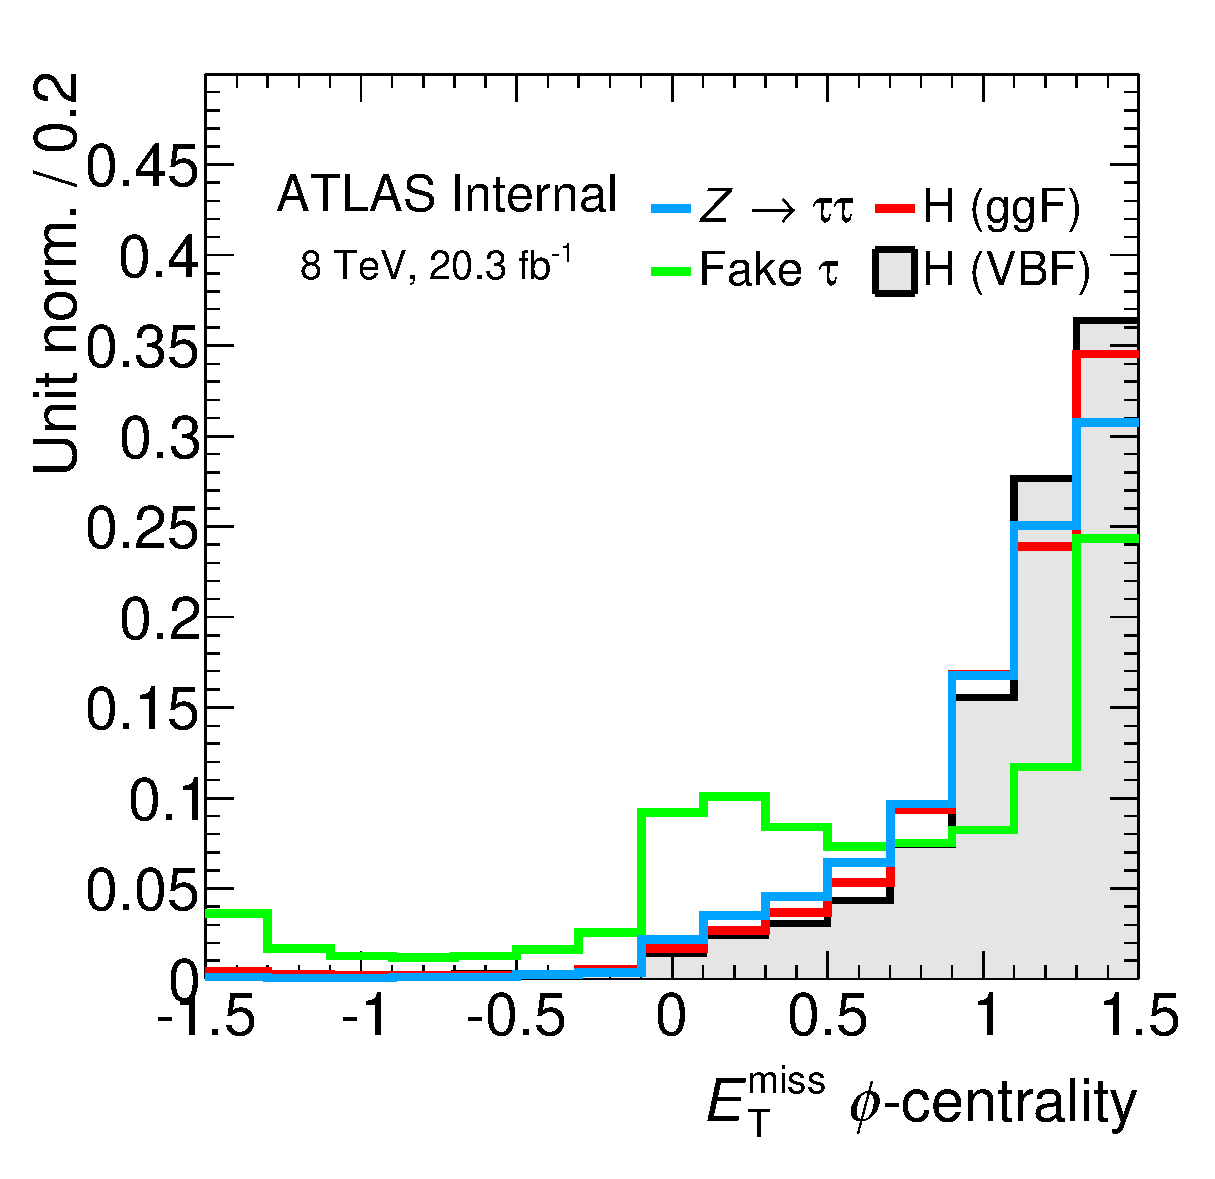
\includegraphics[width=0.32\textwidth]{figures/overlaid/boost/met-phi-centrality}
  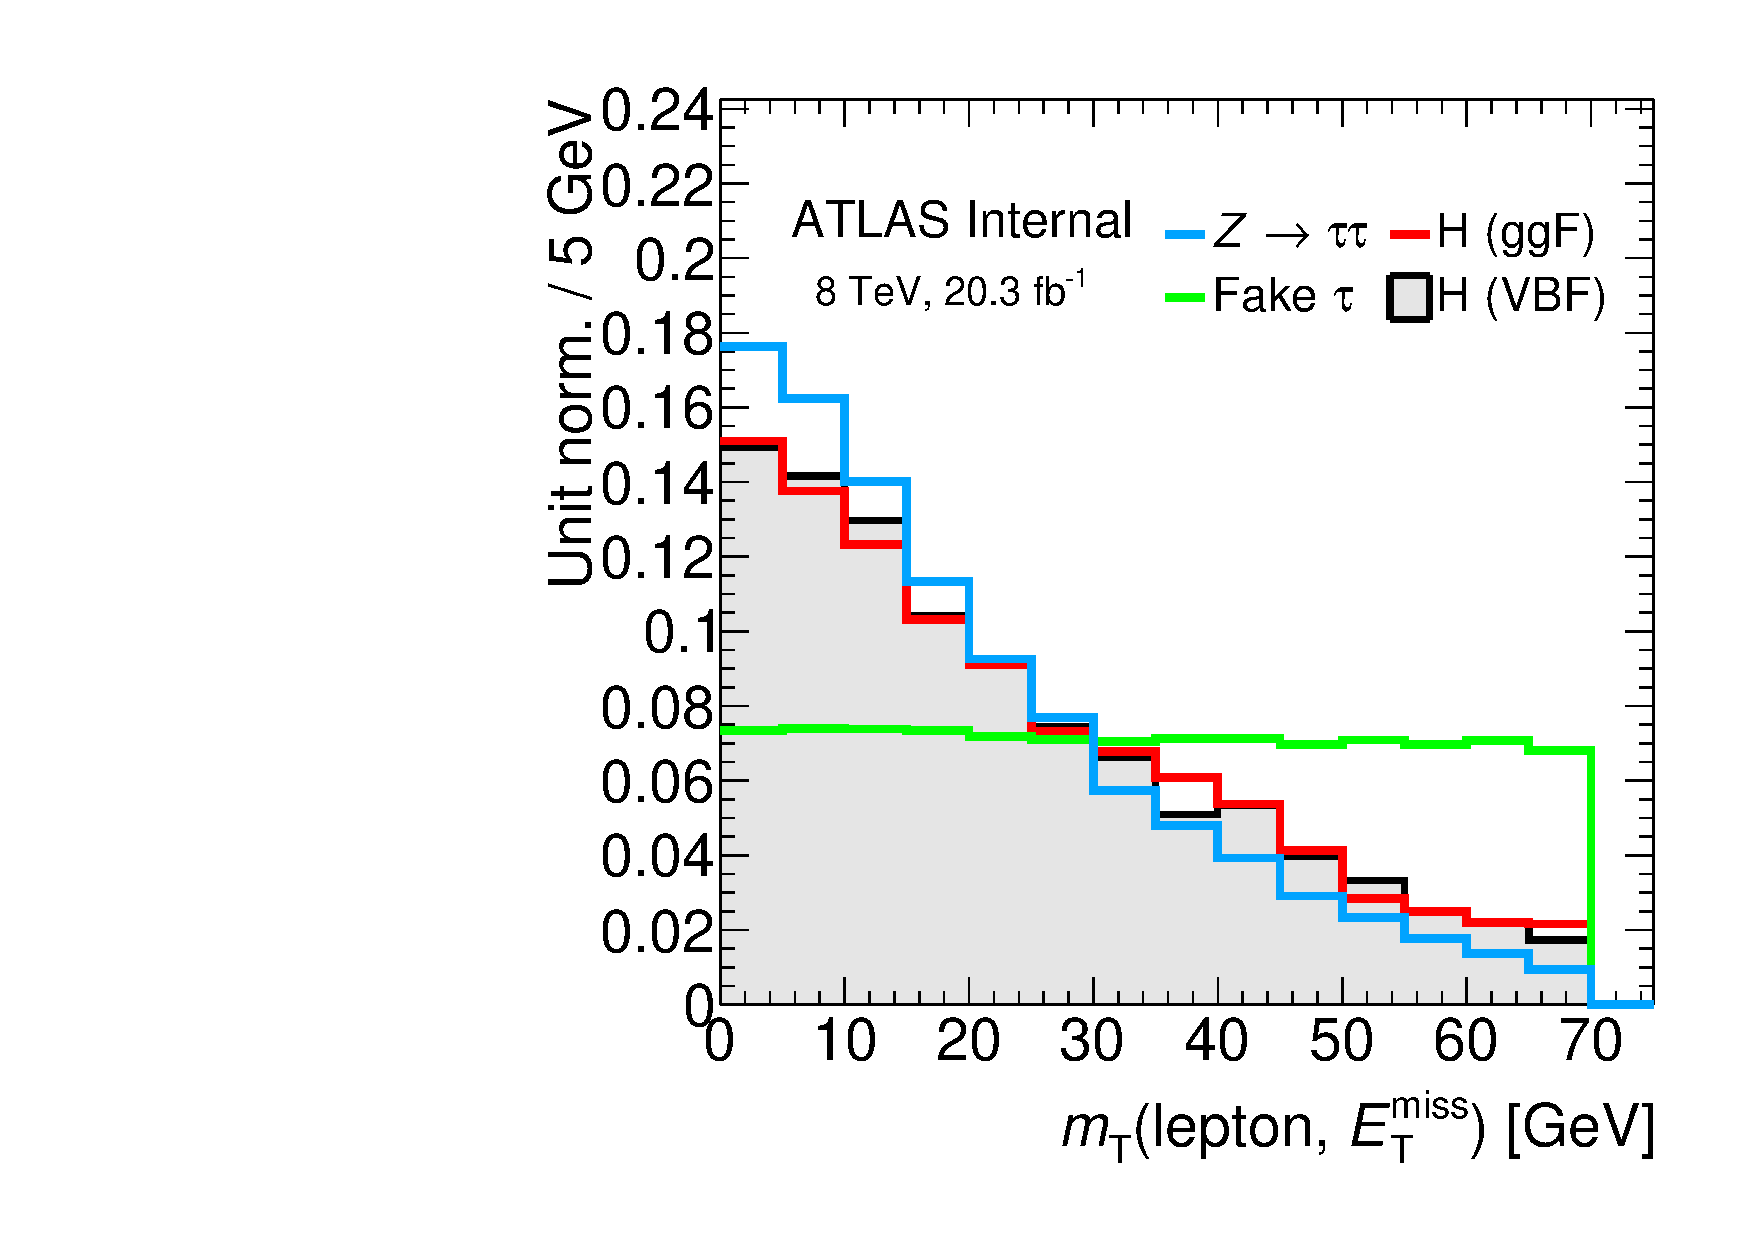
\includegraphics[width=0.32\textwidth]{figures/overlaid/boost/mT} \\
  \caption{Predicted signal and background distributions in the boosted category normalized to unit area and overlaid.}
  \label{fig:strategy-overlaid-boost-1}
\end{figure}
\begin{figure}[tp]
  \centering
  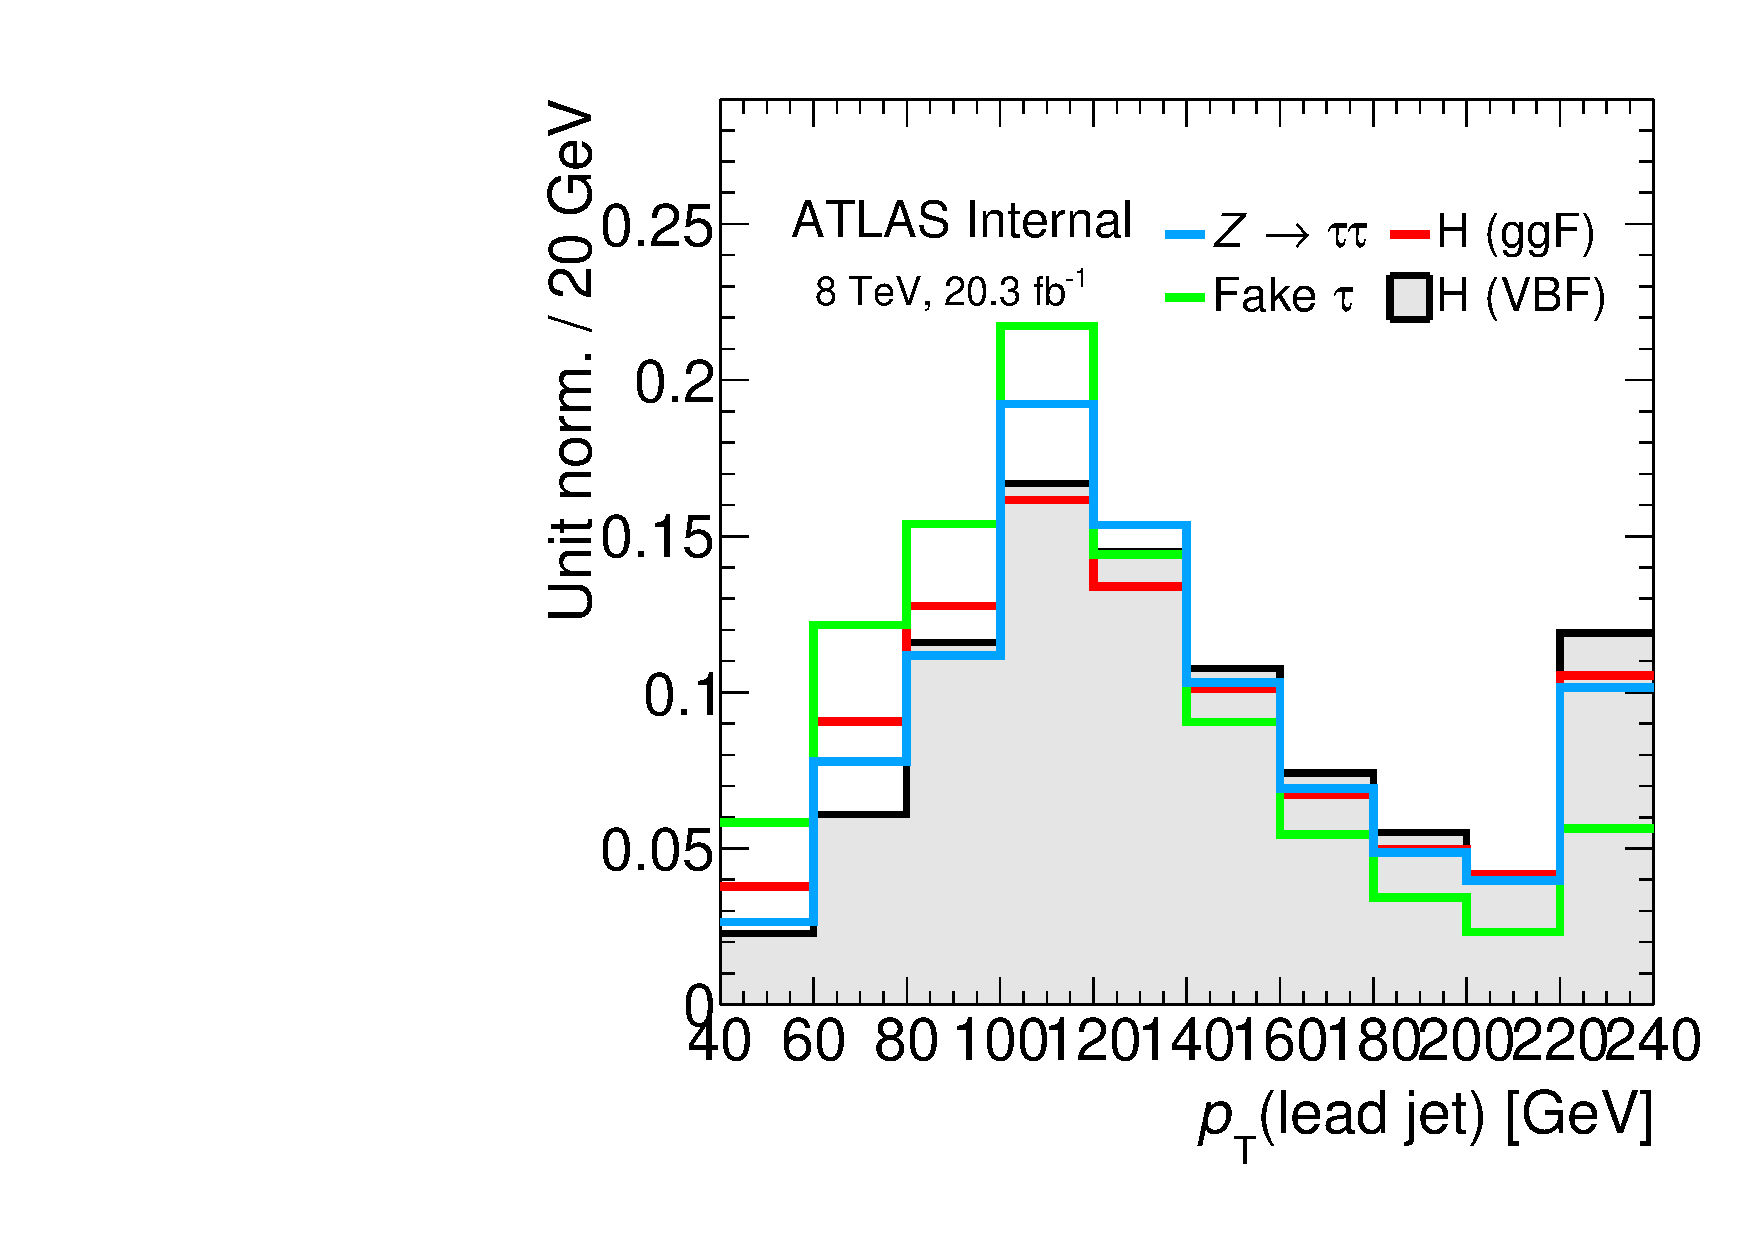
\includegraphics[width=0.32\textwidth]{figures/overlaid/boost/jet-1-pt}
  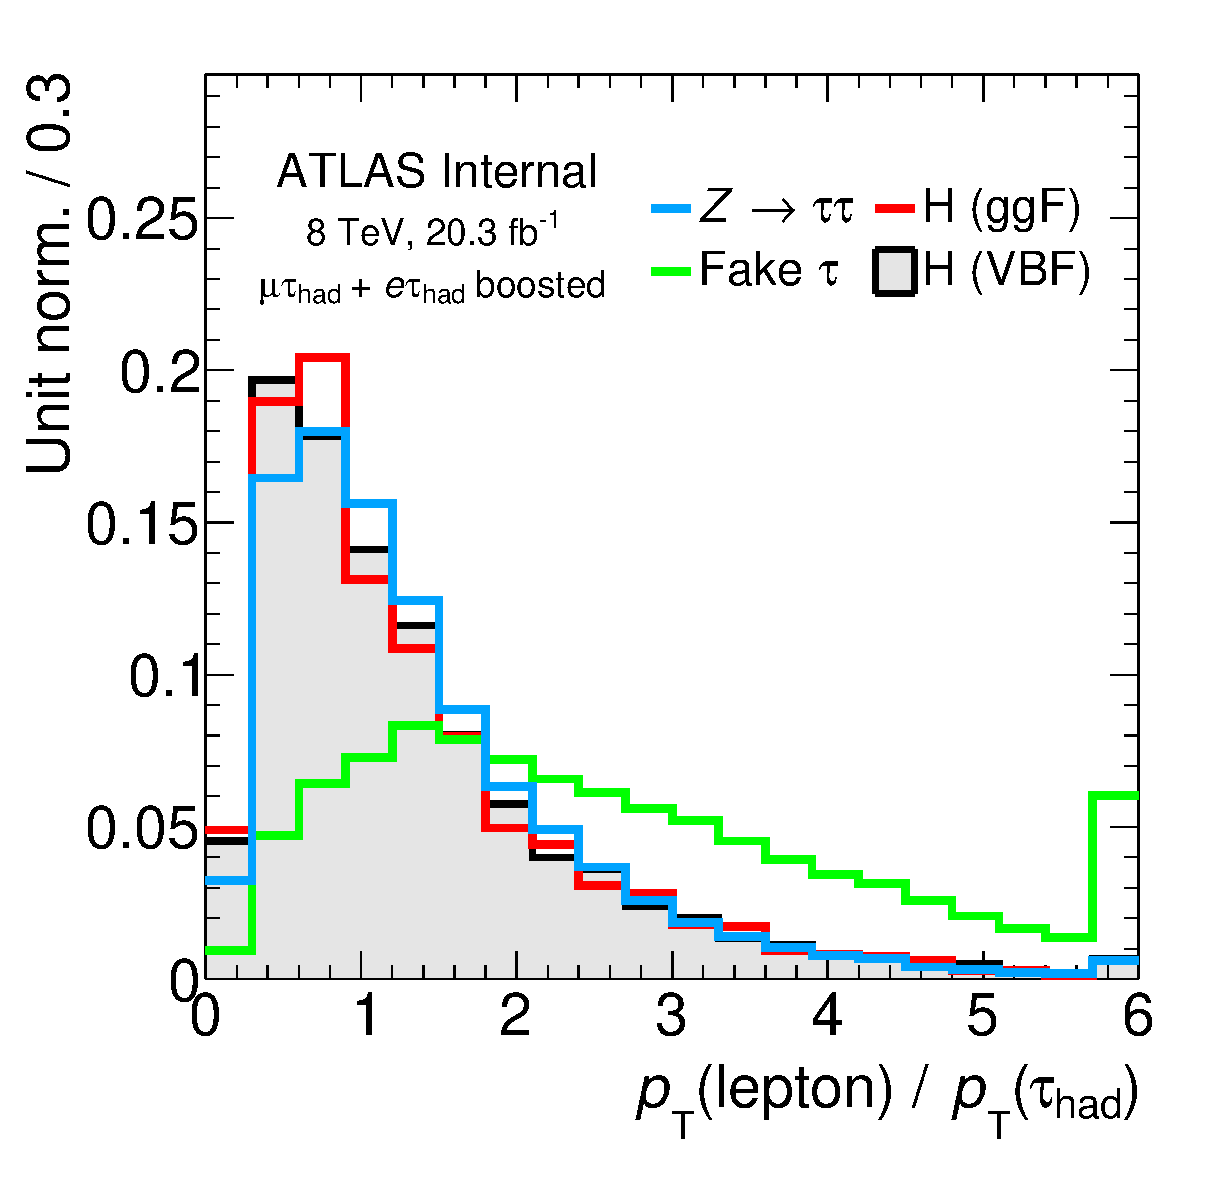
\includegraphics[width=0.32\textwidth]{figures/overlaid/boost/taulep-ptratio}
  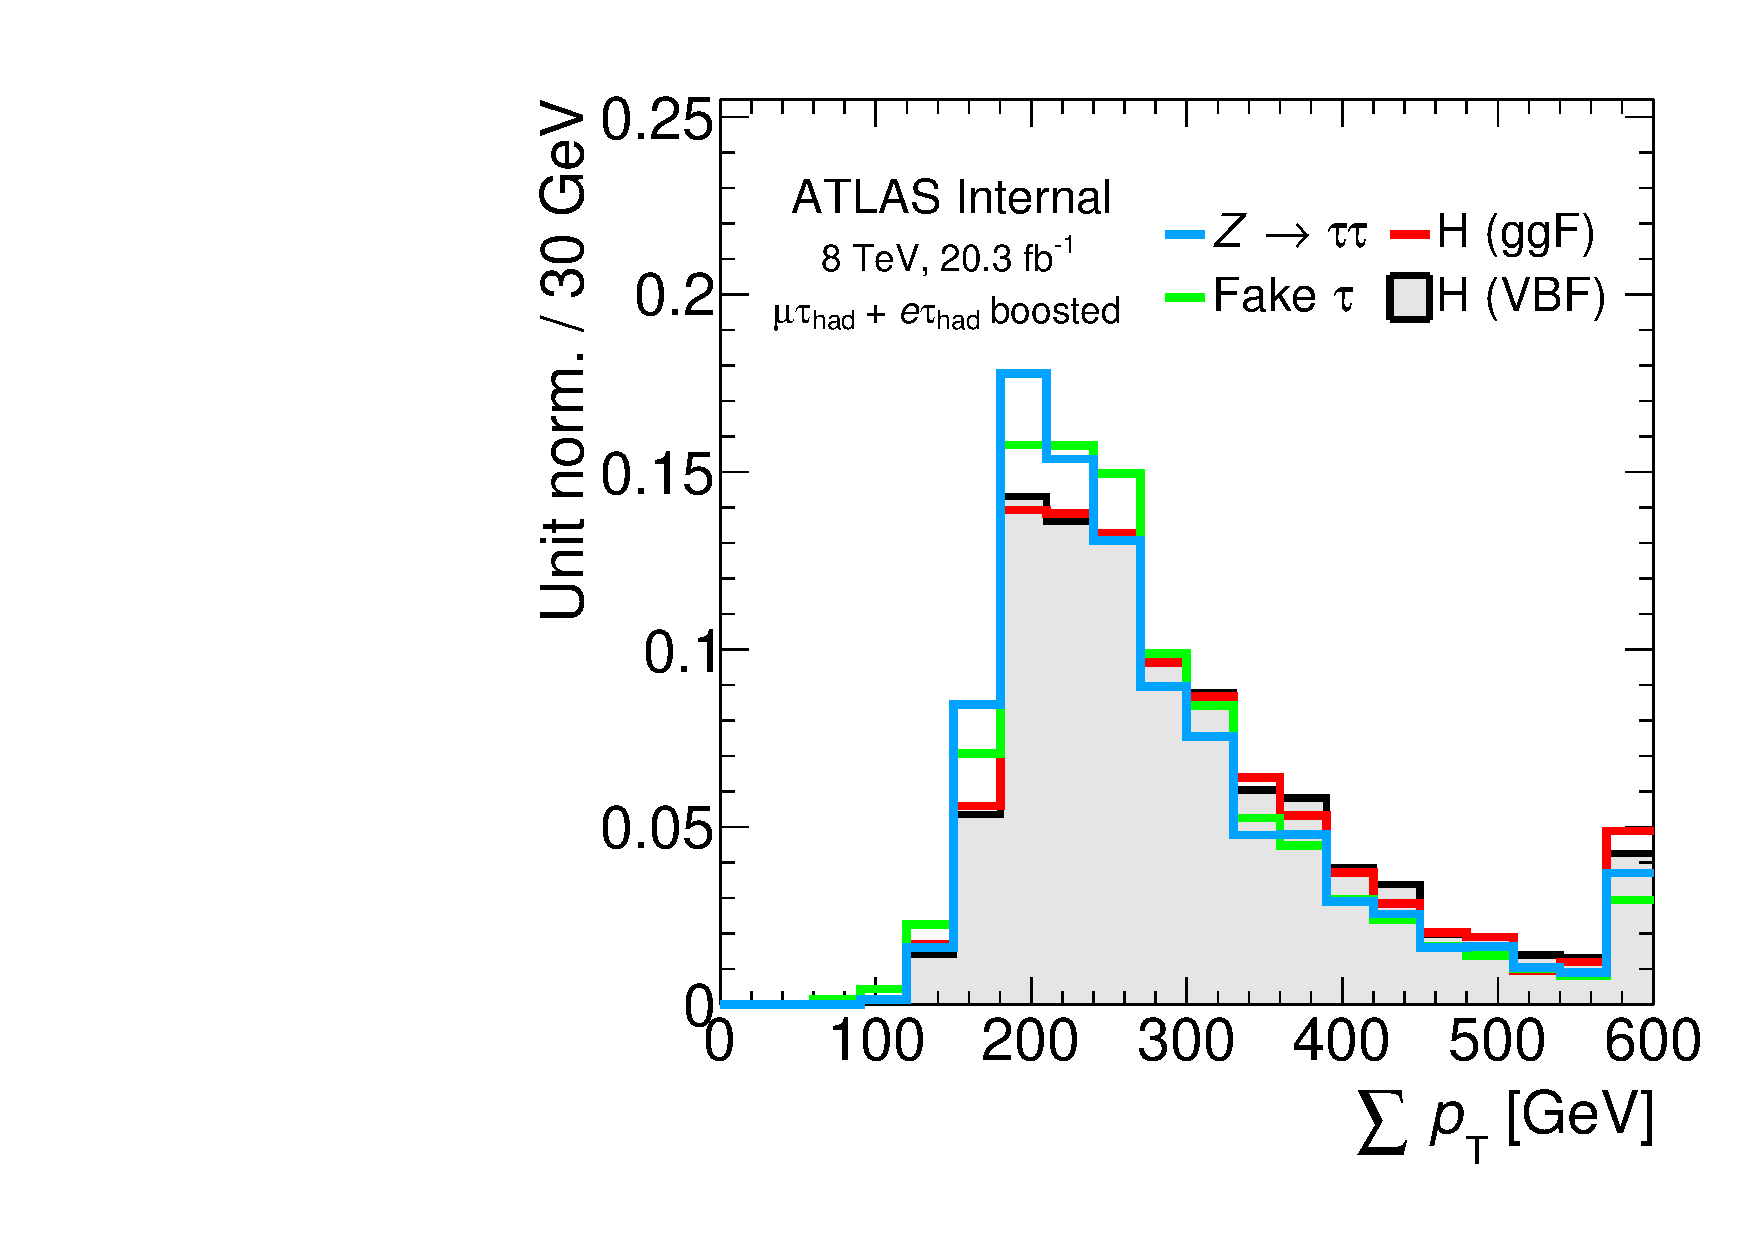
\includegraphics[width=0.32\textwidth]{figures/overlaid/boost/sumpt} \\
  \includegraphics[width=0.32\textwidth]{figures/overlaid/boost/mMMC}
  \includegraphics[width=0.32\textwidth]{figures/overlaid/boost/H-pt-hi}
  \includegraphics[width=0.32\textwidth]{figures/overlaid/boost/BDTEve-boost} \\
  \caption{Predicted signal and background distributions in the boosted category normalized to unit area and overlaid.}
  \label{fig:strategy-overlaid-boost-2}
\end{figure}
% ---------------------------------------------------------------------------------

% VBF
% ---------------------------------------------------------------------------------
\clearpage
\begin{figure}[tp]
  \centering
  \includegraphics[width=0.32\textwidth]{figures/overlaid/vbf/tau-pt}
  \includegraphics[width=0.32\textwidth]{figures/overlaid/vbf/tau-eta}
  \includegraphics[width=0.32\textwidth]{figures/overlaid/vbf/lep-pt-hi} \\
  \includegraphics[width=0.32\textwidth]{figures/overlaid/vbf/lep-eta}
  \includegraphics[width=0.32\textwidth]{figures/overlaid/vbf/tau-numTrack}
  \includegraphics[width=0.32\textwidth]{figures/overlaid/vbf/taulep-dR} \\
  \includegraphics[width=0.32\textwidth]{figures/overlaid/vbf/met-pt-hi}
  \includegraphics[width=0.32\textwidth]{figures/overlaid/vbf/met-phi-centrality}
  \includegraphics[width=0.32\textwidth]{figures/overlaid/vbf/mT} \\
  \caption{Predicted signal and background distributions in the VBF category normalized to unit area and overlaid.}
  \label{fig:strategy-overlaid-vbf-1}
\end{figure}
\begin{figure}[tp]
  \centering
  \includegraphics[width=0.24\textwidth]{figures/overlaid/vbf/jet-1-pt}
  \includegraphics[width=0.24\textwidth]{figures/overlaid/vbf/jet-1-eta}
  \includegraphics[width=0.24\textwidth]{figures/overlaid/vbf/jet-2-pt} 
  \includegraphics[width=0.24\textwidth]{figures/overlaid/vbf/jet-2-eta} \\
  \includegraphics[width=0.24\textwidth]{figures/overlaid/vbf/dijet-m-veryhigh}
  \includegraphics[width=0.24\textwidth]{figures/overlaid/vbf/jets-etaprod}
  \includegraphics[width=0.24\textwidth]{figures/overlaid/vbf/jets-deta} 
  \includegraphics[width=0.24\textwidth]{figures/overlaid/vbf/system-pt} \\
  \includegraphics[width=0.24\textwidth]{figures/overlaid/vbf/lep-eta-centrality}
  \includegraphics[width=0.24\textwidth]{figures/overlaid/vbf/mMMC}
  \includegraphics[width=0.24\textwidth]{figures/overlaid/vbf/H-pt-hi}
  \includegraphics[width=0.24\textwidth]{figures/overlaid/vbf/BDTEve-VBF} \\
  \caption{Predicted signal and background distributions in the VBF category normalized to unit area and overlaid.}
  \label{fig:strategy-overlaid-vbf-2}
\end{figure}
\clearpage

\subsection{Discrimination}
\label{sec:strategy-mva-correlations}

One of the strengths of the BDT analysis is that it can exploit correlations between input variables for better background discrimination. This is especially true in the VBF category where there is interplay between the VBF-oriented variables and the $\Htautau$-oriented variables. Another strength is the BDT can make cuts as hyper-surfaces around weakly discriminating variables instead of rectangular cuts.

Two-dimensional contours of variables of interest are shown in \cref{fig:strategy-kinematic-correlations-1,fig:strategy-kinematic-correlations-2} for VBF $\Htautau$, $\Ztautau$, and $\fakes$. The behavior helps demonstrate the utility of the BDT analysis.
% 
\begin{description}
    \item[$\dR$ and $\mMMC$:] \hfill \\
      $\mMMC$ is not strongly correlated with $\dR$ for $\ZHtautau$ because they are resonant decays. For $\fakes$, there is a strong correlation. 
    \item[$\pt(H)$ and $\dR$:] \hfill \\
      $\dR$ is strongly correlated with $\pt(H)$ for $\ZHtautau$ because their decay products stem from a resonant decay. For $\fakes$, the correlation is weaker.
    \item[$\metphicent$ and $\dR$:] \hfill \\
      $\metphicent$ is correlated with $\dR$ for $\ZHtautau$ because as $\dR$ shrinks, the $\MET$ is more spatially constrained. For $\fakes$, the $\MET$ is more randomly distributed relative to the $\LTT$ system.
    \item[$\mjj$ and $\deta$:] \hfill \\
      For all processes, $\mjj$ and $\deta$ are strongly but not perfectly correlated, hence additional discrimination power is available.
    \item[$\mjj$ and $\dR$:] \hfill \\
      For $\ZHtautau$, there is correlation between $\mjj$ and $\dR$ because the $\tautau$ system is recoiling off of the dijet system. This is an example of interplay between VBF and $\tautau$ kinematics.
    \item[$\mjj$ and $\mMMC$:] \hfill \\
      For all processes, $\mjj$ and $\mMMC$ are not strongly correlated, and their individual discrimination power is comparable. Extracting signal from a fit of the ditau mass is therefore not obviously the best candidate.
\end{description}
%

\clearpage
\begin{figure}[tp]
  \centering
  \includegraphics[width=0.98\textwidth]{figures/kinematiccorrelations/taulep_dR-vs-mMMC} \\
  \includegraphics[width=0.98\textwidth]{figures/kinematiccorrelations/H_pt-vs-taulep_dR} \\
  \includegraphics[width=0.98\textwidth]{figures/kinematiccorrelations/met_phi_cent-vs-taulep_dR} \\
  \caption{Contours of kinematic correlations in the VBF category for VBF $\Htautau$ (left), $\Ztautau$ (center), and fakes (right).}
  \label{fig:strategy-kinematic-correlations-1}
\end{figure}

\begin{figure}[tp]
  \centering
  \includegraphics[width=0.98\textwidth]{figures/kinematiccorrelations/jj_mass-vs-jj_deta} \\
  \includegraphics[width=0.98\textwidth]{figures/kinematiccorrelations/jj_mass-vs-taulep_dR} \\
  \includegraphics[width=0.98\textwidth]{figures/kinematiccorrelations/jj_mass-vs-mMMC} \\
  \caption{Contours of kinematic correlations in the VBF category for VBF $\Htautau$ (left), $\Ztautau$ (center), and fakes (right).}
  \label{fig:strategy-kinematic-correlations-2}
\end{figure}
\clearpage

\subsection{MVAs in other VBF analyses}
\label{sec:strategy-mva-elsewhere}

The $\Htautau$ analysis is one of many recent VBF Higgs analyses on ATLAS to adopt a MVA approach.

In the $\Hyy$ and $\HZZ$ analyses, a VBF BDT is derived which is meant to be uncorrelated with $m_H$. These BDT discriminators use similar input variables as the $\Htautau$ VBF BDT, such as $\mjj$ and $\deta$. For $\Hyy$, a requirement on the output of the BDT discriminator is made ($O_\text{BDT} \ge 0.83$) to enrich the VBF $\Hyy$ process, and the signal is then extracted from a fit of $\myy$. For $\HZZ$, the signal is extracted via a two-dimensional fit of the VBF BDT discriminator and $\mllll$.

The $\HWW$ MVA analysis takes the same approach as the $\Htautau$ analysis. Variables correlated with the reconstructed Higgs mass, including $m_T$ and $\mll$, are included in the BDT discriminator, and the signal yield is extracted from a fit of the BDT output. 

Predicted BDT discriminator outputs are shown in \cref{fig:strategy-elsewhere} for the $\Hyy$, $\HZZ$, and $\HWW$ analyses. Good discrimination is found between signal and background processes. The measured signal strength for these analyses is shown in \cref{tab:strategy-elsewhere}.

\begin{figure}[tp]
  \centering
  \includegraphics[width=0.32\textwidth]{figures/HIGG-2013-08/fig_06}
  \includegraphics[width=0.32\textwidth]{figures/HIGG-2013-21/fig_09f}
  \includegraphics[width=0.32\textwidth]{figures/HIGG-2013-13/fig_46a}
  \caption{Overlaid shapes of BDT outputs for signal and background processes in the VBF $\Hyy$~\cite{HIGG-2013-08}, VBF $\HZZ$~\cite{HIGG-2013-21}, and VBF $\HWW$~\cite{HIGG-2013-13} analyses.}
  \label{fig:strategy-elsewhere}
\end{figure}

\begin{table}[bp]
  \centering
  \renewcommand{\arraystretch}{1.4}
  \caption{Measured VBF signal strength in the other major ATLAS analyses: $\Hyy$~\cite{HIGG-2013-08}, $\HZZ$~\cite{HIGG-2013-21}, and $\HWW$~\cite{HIGG-2013-13}.}
  \begin{tabular}{c|c|c|c}
  channel         & $\Hyy$                 & $\HZZ$                         & $\HWW$ \\
  \hline
  signal strength & $\muVBF = 0.8 \pm 0.7$ & $\muVBFVH = 0.3^{+1.6}_{-0.9}$ & $\muVBF = 1.3 \pm 0.5$ \\
\end{tabular}

  \label{tab:strategy-elsewhere}
\end{table}

